\documentclass[12pt,openany,a4paper]{book}
\usepackage{graphicx}	% if you want encapsulated PS figures.
\usepackage[ddmmyyyy]{datetime}
\usepackage{listings}
\usepackage{tabularx}
\usepackage{dirtree}
\usepackage{url}
% If you use a macro file called macros.tex :
% \input{macros}
% Note: The present document has its macros built in.

% Number subsections but not subsubsections:
\setcounter{secnumdepth}{2}
% Show subsections but not subsubsections in table of contents:
\setcounter{tocdepth}{2}

\pagestyle{headings}		% Chapter on left page, Section on right.
\raggedbottom

\setlength{\topmargin}		{-5mm}  %  25-5 = 20mm
\setlength{\oddsidemargin}	{10mm}  % rhs page inner margin = 25+10mm
\setlength{\evensidemargin}	{0mm}   % lhs page outer margin = 25mm
\setlength{\textwidth}		{150mm} % 35 + 150 + 25 = 210mm
\setlength{\textheight}		{240mm} % 

\renewcommand{\baselinestretch}{1.2}	% Looks like 1.5 spacing.

% Stop figure/tables smaller than 3/4 page from appearing alone on a page:
\renewcommand{\textfraction}{0.25}
\renewcommand{\topfraction}{0.75}
\renewcommand{\bottomfraction}{0.75}
\renewcommand{\floatpagefraction}{0.75}

% THEOREM-LIKE ENVIRONMENTS:
\newtheorem{defn}	{Definition}	% cf. \dfn for cross-referencing
\newtheorem{theorem}	{Theorem}	% cf. \thrm for cross-referencing
\newtheorem{lemma}	{Lemma}		% cf. \lem for cross-referencing

% AIDS TO CROSS-REFERENCING (All take a label as argument):
\newcommand{\eref}[1] {(\ref{#1})}		% (...)
\newcommand{\eq}[1]   {Eq.\,(\ref{#1})}		% Eq.~(...)
\newcommand{\eqs}[2]  {Eqs.~(\ref{#1}) and~(\ref{#2})}
\newcommand{\dfn}[1]  {Definition~\ref{#1}}	% Definition~...
\newcommand{\thrm}[1] {Theorem~\ref{#1}}	% Theorem~...
\newcommand{\lem}[1]  {Lemma~\ref{#1}}		% Lemma~...
\newcommand{\fig}[1]  {Fig.\,\ref{#1}}		% Fig.~...
\newcommand{\tab}[1]  {Table~\ref{#1}}		% Table~...
\newcommand{\chap}[1] {Chapter~\ref{#1}}	% Chapter~...
\newcommand{\secn}[1] {Section~\ref{#1}}	% Section~...
\newcommand{\ssec}[1] {Subsection~\ref{#1}}	% Subsection~...
\newcommand{\app}[1]  {Appendix~\ref{#1}}	% Appendix~...

% AIDS TO FORMATTING:
\newcommand{\teq}[1]	{\mbox{$#1$}}	% in-Text EQuation (unbreakable)
\newcommand{\qed}	{\hspace*{\fill}$\bullet$}	% end of proof

% MATHEMATICAL TEMPLATES:
% Text or math mode:
\newcommand{\half}	{\ensuremath{\frac{1}{2}}}	% one-half
\newcommand{\halftxt}	{\mbox{$\frac{1}{2}$}}	  	% one-half, small
% Math mode only:
% N.B. Parentheses are ROUND; brackets are SQUARE!
\newcommand{\oneon}[1]	{\frac{1}{#1}}		  % reciprocal
\newcommand{\pow}[2]	{\left({#1}\right)^{#2}}  % Parenthesized pOWer
\newcommand{\bow}[2]	{\left[{#1}\right]^{#2}}  % Bracketed pOWer
\newcommand{\evalat}[2]	{\left.{#1}\right|_{#2}}  % EVALuated AT with bar
\newcommand{\bevalat}[2]{\left[{#1}\right]_{#2}}  % Bracketed EVALuated AT
% Total derivatives:
\newcommand{\sdd}[2]	{\frac{d{#1}}{d{#2}}}		    % Short
\newcommand{\sqdd}[2]	{\frac{d^2{#1}}{d{#2}^2}}	    % 2nd ("SQuared")
\newcommand{\ldd}[2]	{\frac{d}{d{#1}}\left({#2}\right)}  % Long paren'ed
\newcommand{\bdd}[2]	{\frac{d}{d{#2}}\left[{#2}\right]}  % long Bracketed
% Partial derivatives (same sequence as for total derivatives):
\newcommand{\sdada}[2]	{\frac{\partial {#1}}{\partial {#2}}}
\newcommand{\sqdada}[2]	{\frac{\partial ^{2}{#1}}{\partial {#2}^{2}}}
\newcommand{\ldada}[2]	{\frac{\partial}{\partial {#1}}\left({#2}\right)}
\newcommand{\bdada}[2]	{\frac{\partial}{\partial {#1}}\left[{#2}\right]}
\newcommand{\da}	{\partial}

% ORDINAL NUMBERS:
\newcommand{\ith}	{\ensuremath{i^{\rm th}}}
\newcommand{\jth}	{\ensuremath{j^{\rm th}}}
\newcommand{\kth}	{\ensuremath{k^{\rm th}}}
\newcommand{\lth}	{\ensuremath{l^{\rm th}}}
\newcommand{\mth}	{\ensuremath{m^{\rm th}}}
\newcommand{\nth}	{\ensuremath{n^{\rm th}}}

% SINUSOIDAL TIME AND SPACE-DEPENDENCY FACTORS:
\newcommand{\ejot}	{\ensuremath{e^{j\omega t}}}
\newcommand{\emjot}	{\ensuremath{e^{-j\omega t}}}

% UNITS (TEXT OR MATH MODE, WITH LEADING PADDING SPACE IF APPLICABLE):
% NB: These have not been tested since being modified for LaTeX2e.
\newcommand{\pack}	{\hspace{-0.08em}}
\newcommand{\Pack}	{\hspace{-0.12em}}
\newcommand{\mA}	{\ensuremath{\rm\,m\pack A}}
\newcommand{\dB}	{\ensuremath{\rm\,d\pack B}}
\newcommand{\dBm}	{\ensuremath{\rm\,d\pack B\pack m}}
\newcommand{\dBW}	{\ensuremath{\rm\,d\pack B\Pack W}}
\newcommand{\uF}	{\ensuremath{\rm\,\mu\pack F}}
\newcommand{\pF}	{\ensuremath{\rm\,p\pack F}}
\newcommand{\nF}	{\ensuremath{\rm\,n\pack F}}
\newcommand{\uH}	{\ensuremath{\rm\,\mu\pack H}}
\newcommand{\mH}	{\ensuremath{\rm\,m\pack H}}
\newcommand{\Hz}	{\ensuremath{\rm\,H\pack z}}
\newcommand{\kHz}	{\ensuremath{\rm\,k\pack H\pack z}}
\newcommand{\MHz}	{\ensuremath{\rm\,M\pack H\pack z}}
\newcommand{\GHz}	{\ensuremath{\rm\,G\pack H\pack z}}
\newcommand{\J}		{\ensuremath{\rm\,J}}
\newcommand{\kg}	{\ensuremath{\rm\,k\pack g}}
\newcommand{\K}		{\ensuremath{\rm\,K}}
\newcommand{\m}		{\ensuremath{\rm\,m}}
\newcommand{\cm}	{\ensuremath{\rm\,cm}}
\newcommand{\km}	{\ensuremath{\rm\,k\pack m}}
\newcommand{\mm}	{\ensuremath{\rm\,m\pack m}}
\newcommand{\nm}	{\ensuremath{\rm\,n\pack m}}
\newcommand{\um}	{\ensuremath{\rm\,\mu m}}
\newcommand{\Np}	{\ensuremath{\rm\,N\pack p}}
\newcommand{\s}		{\ensuremath{\rm\,s}}
\newcommand{\ms}	{\ensuremath{\rm\,m\pack s}}
\newcommand{\us}	{\ensuremath{\rm\,\mu s}}
\newcommand{\V}		{\ensuremath{\rm\,V}}
\newcommand{\mV}	{\ensuremath{\rm\,m\Pack V}}
\newcommand{\W}		{\ensuremath{\rm\,W}}
\newcommand{\mW}	{\ensuremath{\rm\,m\Pack W}}
\newcommand{\ohm}	{\ensuremath{\rm\,\Omega}}
\newcommand{\kohm}	{\ensuremath{\rm\,k\Omega}}
\newcommand{\Mohm}	{\ensuremath{\rm\,M\Omega}}
\newcommand{\degs}	{\ensuremath{\rm^{\circ}}}

% LaTeX run-time type-in command:
%
% \typein{Enter \protect\includeonly{...} command (or just type RETURN):}
%
% Uncommenting this command makes LaTeX prompt you for the \includeonly
% list.  At the prompt
%
%	\@typein=
%
% you type
%
%	\includeonly{chap1,chap2}
%
% to include the files chap1.tex and chap2.tex and omit any others.
% To include every \include file, just hit RETURN.
% If you are running LaTeX from xtexsh, you may need to click the mouse
% in the LaTeX window to position the cursor at the \@typein prompt.

\begin{document}

\frontmatter
% By default, frontmatter has Roman page-numbering (i,ii,...).

\begin{titlepage}
\renewcommand{\baselinestretch}{1.0}
\begin{center}
\centerline{
\includegraphics{PNGLogo.png}}
\vspace*{35mm}
\Huge\bf
		Smart\\
		Beach Mat\\
\vspace{20mm}
\large\sl
		by\\
		Adam Dorogi-Kaposi
		\medskip\\
\rm
		School of Information Technology and Electrical Engineering,\\
		The University of Queensland.\\
\vspace{30mm}
		Submitted for the degree of\\
		Bachelor of Engineering (Honours)
		\smallskip\\
\normalsize
		in the field of Software Engineering.
		\medskip\\
\large
		November, 2019.
\end{center}
\end{titlepage}

\cleardoublepage

\begin{flushright}
	U5803, 501 Adelaide Street\\
	Brisbane City, QLD 4000\\
	Tel.\ (04) 0435 5180\\
	\medskip
	\today
\end{flushright}
\begin{flushleft}
  Prof Amin Abbosh\\
  Acting Head of School\\
  School of Information Technology and Electrical Engineering\\
  The University of Queensland\\
  St Lucia, QLD 4072\\
  \bigskip\bigskip
  Dear Professor Abbosh,
\end{flushleft}

In accordance with the requirements of the degree of Bachelor of
Engineering (Honours) in the division of Software Engineering, I present the
following thesis entitled ``Smart Beach Mat''.  This work was performed under
the supervision of Dr Alex Pudmenzky.

I declare that the work submitted in this thesis is my own, except as
acknowledged in the text and footnotes, and has not been previously
submitted for a degree at The University of Queensland or any other
institution.

\begin{flushright}
	Yours sincerely,\\
	\medskip
	\emph{}\\
	\medskip
	Adam Dorogi-Kaposi
\end{flushright}

\cleardoublepage

% % Dedication (if you want it):
% \vspace*{70mm}
% \begin{center}
% \renewcommand{\baselinestretch}{1.0}
% \sl
% 	To \ldots
% \end{center}

\chapter{Acknowledgments}

I'd like to thank my supervisor, Dr Alex Pudmenzky, for the continuous support
and guidance throughout the duration of the thesis project. More specifically,
I'd like to thank him for giving me the opportunity to work on this project,
for consistently keeping me on track, and for contributing ideas which helped
shaped the outcomes. 

I'd also like to thank the project client, Dr Tushar Kumeria, for
contributing countless innovative ideas, for keeping me motivated through his
passion, and for all the valuable brainstorming sessions.

Finally, I'd like to thank my family and friends for their continuous support
and motivation, and their valuable input to project related discussions.

\cleardoublepage

\chapter{Abstract}

% Notice that all \include files are chapters -- a logical division.
% But not all chapters are \include files; some chapters are short
% enough to be in-lined in the main file.

This thesis project aims to raise awareness of ultraviolet (UV) radiation, and
guide people in tracking their UV exposure with the help of an Internet
of Things (IoT) device and a smartphone application. This project aims to alert
product users of dangerous sun exposure levels based on their skin type, skin
conditions, gender, and age.

To achieve this purpose, two products were developed
using multiple hardware components, and open-source software frameworks. Product
validation and user research has also been conducted, and the Scrum software
development process has been used throughout the project.

The outcomes of this project were two products: an IoT device relying on UV
sensing hardware, and a cross-platform smartphone application. Both products
rely on Bluetooth Low Energy for communication between one another. The
smartphone application also communicates with a server to store user related
data, such as UV readings, on the cloud.

\tableofcontents

\listoffigures
\addcontentsline{toc}{chapter}{List of Figures}

\listoftables
\addcontentsline{toc}{chapter}{List of Tables}

% If file los.tex begins with ``\chapter{List of Symbols}'':
% \include{los}

\cleardoublepage

\mainmatter
% By default, mainmatter has Arabic page-numbering (1,2,...).


% Chapters may be \include files, each beginning with a line like
%
%	\chapter{Title of chapter}
%
% e.g. if two chapter files were called intro.tex and theory.tex,
% we would say
%
%	\include{intro}
%	\include{theory}

\chapter{Introduction}

As of 2018, Australia is the leading country for skin cancer rates for both
sexes~\cite{bray_2018}. Australia's ozone layer has thinned by 5--9\% since 1960,
resulting in increased exposure to the sun's harmful UVB radiation~\cite{department_ee}.
Since prolonged UVB radiation has been linked to skin cancer~\cite{twenty_one_q}, this
project aims to raise awareness of such radiation by developing two products
which help visualise and track their users' UV exposure.

This thesis project consists of two components:
\begin{enumerate}
	\item an IoT device with a UV sensing component; and
	\begin{itemize}
		\item Intended to be clipped on to a beach mat, hence the name ``Smart
		Beach Mat''.
	\end{itemize}
	\item a smartphone application.
	\begin{itemize}
		\item Receives and displays data (such as UV readings) from the IoT
		device, and stores certain data on the server.
	\end{itemize}
\end{enumerate}
With the help of these two products, this project aims to guide its users in
tracking their UV exposure in hopes of preventing UV related skin diseases,
such as skin cancer. The smartphone application also aims to alert its users
after prolonged sun exposure, which will be determined using formulas based on
the users' skin type, gender, and age.

This thesis covers the hardware and firmware development of the IoT device, and
the front-end software development of the smartphone application. The scope also
covers the development of a REST API to communicate with the smartphone, and the
design and implementation of a remote database to store user related information.

The remainder of the thesis includes extending the smartphone application with
more features, such as visualising UV exposure history. Remaining work on the
hardware includes making the device casing waterproof, and creating an
all-in-one PCB which combines all the components from the separate break-out
boards. A detailed explanation of future work can be found in
\secn{secn:future_work}.

% \textbf{Thesis definition and scope (10\%):} A clear definition of a substantial and
% significant topic, problem and/or hypothesis and the thesis scope should leave
% the reader with no doubt about the scope, purpose, relevance, context and
% contribution of the thesis. The thesis definition and scope should relate to the
% literature, and show the assumptions (or challenges to assumptions) that have
% been identified. The scope should require a substantial effort (see Approach and
% execution below).

\cleardoublepage

\chapter{Background}

% \textbf{Background (20\%):} Background material for the thesis should likely include
% reviews, analyses and discussions of the literature in the area of the thesis
% and about methods applicable to achieving the thesis goals. This background
% should not only help the reader understand the rest of the document, but should
% illustrate to the reader a clear mastery of the material in the topic area and
% an ability to synthesize and abstract knowledge from other sources.

% \bigskip

% You will need to review previous work in the field, which may include
% books and papers (``literature''), patents and commercial products
% (``prior art''), and earlier work in your Department.  This
% information is usually (but not always) collected in a single chapter,
% whose title should preferably be more specific and interesting than
% the one above.

\section{UV Radiation}

UV radiation, or UV light, is (invisible) electromagnetic radiation produced by the
sun, in the wavelength range of 10--400\nm~\cite{cancer_council}. The three main subtypes of UV
radiation are UVA, UVB, and UVC radiation~\cite[\tab{tab:uv_radiation}]{spacewx}.

\begin{table}[h]
\caption{\sl Three main subtypes of the electromagnetic spectrum of UV
radiation.}
\label{tab:uv_radiation}
\begin{center}
\begin{tabular}{|c|c|c|}
\hline
Subtype & Wavelength (nm) & Photon Energy (eV) \\
\hline
UVA & 315--400 & 3.10--3.94 \\
UVB & 280--315 & 3.94--4.43 \\
UVC & 100--280 & 4.43--12.4 \\
\hline
\end{tabular}
\end{center}
\end{table}

UVA and UVB radiation both reach the Earth's surface, whereas UVC radiation is
completely absorbed by the atmosphere and ozone layer. UV radiation is
known to cause cancer, and is therefore considered a human carcinogen~\cite{cancer_council}.

Overexposure to UV light damages DNA and skin cells, resulting in common
symptoms such as a suntan or sunburn. This skin damage increases the risk of skin
cancer, and affects all skin types~\cite{nasa}; however, certain skin types have
different thresholds for UV exposure, and may be affected faster or slower than
other skin types (see \secn{secn:fitzpatrick_scale}).

It's also worth noting that, even though it may seem like it, UV radiation is
\emph{not} related to temperature, and one \emph{cannot} feel UV
radiation~\cite{cancer_council}. Since there are no immediate effects of UV exposure, its
presence is often easy to forget about until skin damage has occured.

\section{UV Index}

The UV Index is a standard measurement of UV radiation at a particular place and
time. It's an open-ended linear scale ranging from zero to 11+, and is directly
proportional to the amount of UV radiation required for human sunburn~\cite{australia_government}.
As an example, if a person gets sunburnt in 40 minutes at UV Index five, the same
person would get sunburnt in 20 minutes at UV Index ten. The higher the UV Index,
the faster the rate of damage on the skin.

UV Index values are often categorised into specific ranges, to help the
general public understand their severity~\cite[\fig{fig:uv_index}]{foresthill_weather}.

\begin{figure}[h]
\centerline{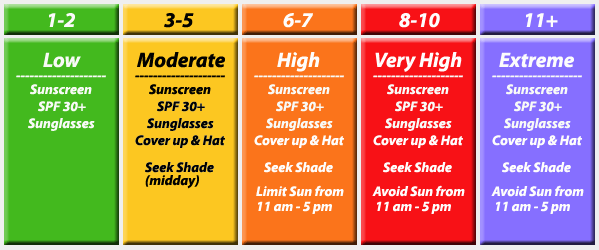
\includegraphics[width=\textwidth]{UVIndex.png}}
\caption{The UV Index ranges}
\label{fig:uv_index}
\end{figure}

The smartphone application will display UV Index values, along with their
severity classifications, to help users understand the severity and meaning of
the current UV Index.

\section{Fitzpatrick Scale}
\label{secn:fitzpatrick_scale}

The Fitzpatrick scale is a classification schema for human skin colour in the
range one to six (I to VI). The scale indicates different skin types' response to UV
radiation ~\cite[\fig{fig:fitzpatrick_scale}]{dorazio_2013}, and classifies skin
colours into one of six categories~\cite{skin_inc}:
\begin{enumerate}
	\item Type I
	\begin{itemize}
		\item always burns, never tans (palest, freckly skin type)
	\end{itemize}
	\item Type II
	\begin{itemize}
		\item usually burns, tans minimally
	\end{itemize}
	\item Type III
	\begin{itemize}
		\item sometimes burns mildly, tans evenly
	\end{itemize}
	\item Type IV
	\begin{itemize}
		\item burns minimally, always tans well (moderate brown skin type)
	\end{itemize}
	\item Type V
	\begin{itemize}
		\item burns rarely, tans easily (dark brown skin type)
	\end{itemize}
	\item Type VI
	\begin{itemize}
		\item never burns (deeply pigmented, darkest brown skin type)
	\end{itemize}
\end{enumerate}

\begin{figure}[h]
\centerline{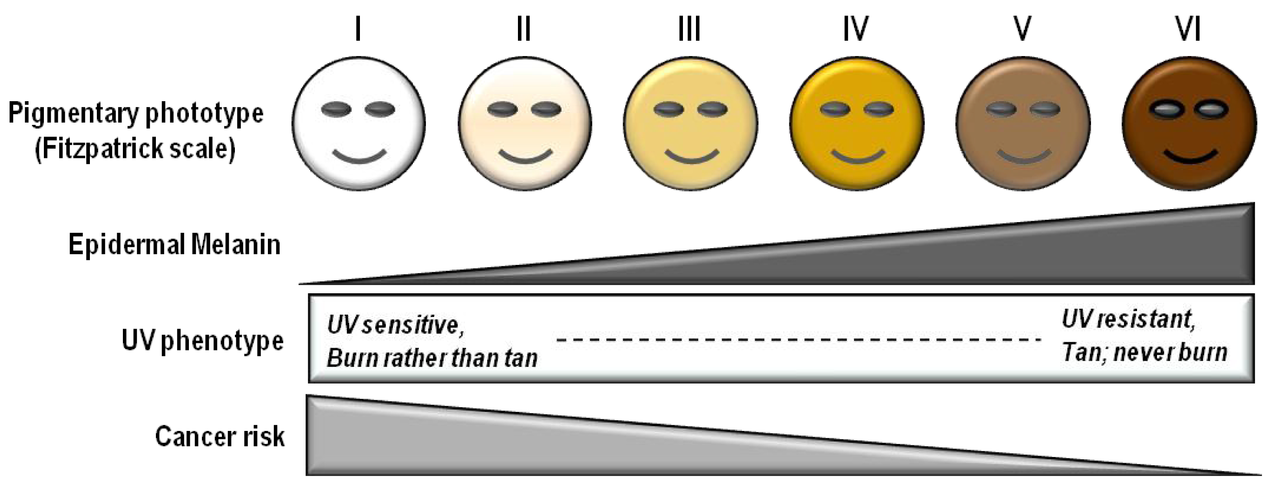
\includegraphics[width=\textwidth]{FitzpatrickScale.png}}
\caption{The Fitzpatrick scale and the risk of skin cancer}
\label{fig:fitzpatrick_scale}
\end{figure}

The Fitzpatrick scale plays an important role in estimating each skin type's threshold to
UV radiation, and will be considered in the smartphone application for such
estimations.

\section{Relevant Technologies}

\subsection{Bluetooth Low Energy}

Bluetooth Low Energy (BLE), is a wireless communication technology used for
short range communication between BLE compatible devices, such as a smartphone
and a BLE enabled blood pressure monitor. Bluetooth operates in the
2400--2483.5\MHz\ range, in the 2.4\GHz\ Industrial, Scientific and Medical (ISM)
radio frequency band~\cite{ray_2015}.

Due to BLE's low power consumption, devices
exchanging small amounts of periodic data may run on a small battery for years~\cite{ray_2015},
making it a suitable communication protocol for this thesis project. BLE's short
range communication also comes with the benefit of relatively high data-transfer
rates (1 Mb/s), making it more suitable for IoT devices~\cite{ray_2015}.

\subsection{Hypertext Transfer Protocol}

Similarly to BLE, Hypertext Transfer Protocol (HTTP) is a standardised
communication protocol that can also be used to wirelessly transmit data between
a client and a server, such as a smartphone and a web server~\cite{W3schools}.
Unlike BLE however, HTTP is used to communicate over the Internet, which typically
happens over a long range --- between countries.

Like most communication protocols, HTTP communication is made up of HTTP requests
--- from the client to the server ---  and HTTP responses --- from the server to
the client. Each HTTP request defines a specific HTTP request method, which
indicates the desired action to be performed by the server upon receiving the
request~\cite{mdn_http_methods}. Common examples of HTTP methods
include~\cite{mdn_http_methods, shuler_2002}:
\begin{itemize}
	\item \verb|GET|
	\begin{itemize}
		\item Used to request a resource from the server, and should only be
		used to retrieve data.
		\item Example: Requesting the homepage of Wikipedia.
	\end{itemize}
	\item \verb|POST|
	\begin{itemize}
		\item Used to submit a resource to the server, often resulting in a
		created resource on --- or a changed state of --- the server.
		\item Example: Submitting an online survey.
	\end{itemize}
	\item \verb|PUT|
	\begin{itemize}
		\item Used to completely replace a resource on the server.
		\item Example: Update your Google account information.
	\end{itemize}
	\item \verb|DELETE|
	\begin{itemize}
		\item Used to delete a resource from the server.
		\item Example: Delete a question posted to Piazza.
	\end{itemize}
\end{itemize}
The HTTP response is the response that is sent back to
the client, following the client's HTTP request. A response is used to indicate
the status of the request with a status code --- such as a \verb|200 OK| status
code indicating successful request completion --- and optionally return data to
the client~\cite{shuler_2002}.

% TODO
% \subsubsection{REST API}

% A representational state transfer (REST) application programming interface (API)
% is a

\subsection{Flutter}

Flutter is a framework for the Dart programming language developed by Google in
2017~\cite{bracken_2018}. It can be used to create beautiful, cross-platform
smartphone
applications in record time ~\cite{flutter_dev_intro}, allowing fast development, an expressive
and flexible user interface (UI), and native performance.

Dart is a functional programming language, and with the use of the Flutter framework,
introduces a ``hot reload'' feature, used during smartphone application development.
This feature preserves the state of your application, enabling you to view the
effect of changed code almost immediately, without having to completely rebuild
the project~\cite{flutter_dev_hot_reload}.

These features may save countless hours of development time, and a wider market
due to the cross-platform capabilities. Since Flutter has been designed to get
something out the door as fast as possible, it will be used to develop the
smartphone application for the thesis project.

\subsection{PHP}
\label{secn:php}

PHP is a scripting language, often used on web servers to develop back-end
(server-side) functionality. It can be used for web development, for example,
by embedding PHP in static HTML web pages. This results in the web page being
generated ``on the fly''
after a client makes a HTTP \verb|GET| request, and the newly generated web page
is returned to the client. PHP has other use cases, such as connecting to and
manipulating remote databases.

Due to its features and flexibility, PHP is often used to generate HTML pages
based on contents of databases, such as displaying a list of users on a web
page~\cite{php_intro}. In other words, PHP is often used to link the client's HTTP
requests to a database operation, optionally returning a database record to the
client. PHP can accept any HTTP request, which doesn't necessarily have to come
from a webpage; the request can also come from other sources, such as desktop
or smartphone applications, and IoT devices.

Due to previous experience, its simple syntax, and its vast documentation, PHP
will be used as the server-side programming language to handle API calls for
this thesis project.

\subsection{MySQL}

MySQL is an open-source Structured Query Language (SQL) database management
system. It's used to define relational databases, meaning the relationships between each
entity in the database is defined during the construction of the database. A MySQL
database is made up of multiple, user-defined tables, corresponding to entities
in the database. Each row in a table represents an instance of data, and the
column names represent the different attributes of that data~\cite{mysql_intro}.
For example, a database may contain a table called \verb|users|, having columns
\verb|name|, \verb|gender|, and \verb|dob|. The table may contain
the following rows:
\begin{verbatim}
John, Male, 21-03-1996
Mary, Female, 09-11-1999
\end{verbatim}

MySQL is often used to store information for web applications, such as usernames,
passwords, or products in an online store. These database entries can be created,
retrieved, updated, and deleted either manually through a database management interface
--- such as PHPMyAdmin --- or by using a server-side programming language, such as PHP
(see \secn{secn:php}).

The database schema --- or the relations between database tables --- are often expressed
using entity-relationship (ER) diagrams. ER diagrams define the entities in a database
using rectangles, the relationships between entities using diamonds, and the attributes
of the entities using ovals. En example of an ER diagram
can be seen in~\cite[\fig{fig:er_diagram_example}]{kandasamy_2016}.

\begin{figure}[h]
\centerline{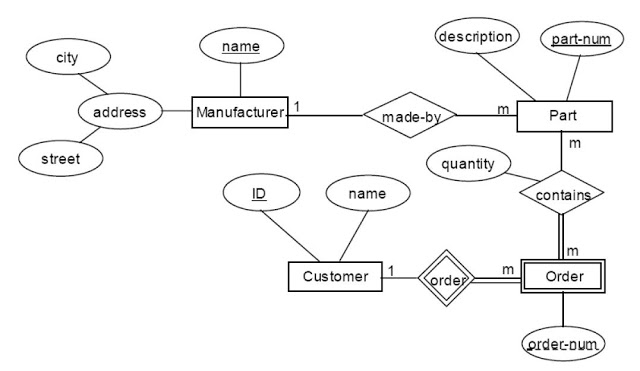
\includegraphics[width=0.8\textwidth]{ERDiagramExample.jpg}}
\caption{Example ER diagram}
\label{fig:er_diagram_example}
\end{figure}


\section{Prior Art}
\label{secn:prior_art}

\subsection{Shade}

Shade is an ultra-accurate clinical-grade wearable UV sensor, backed by the
National Cancer Institute (USA), and the National Science Foundation
(USA)~\cite{wearshade_intro}. This
wearable piece of technology, clipped to clothing by magnets, empowers anyone to
proactively manage sun exposure, and is proved to be 5--30 times more accurate
than other UV wearable according to their publication ``A Comparative Study of
Wearable Ultraviolet Radiometers''~\cite{banerjee}.

The paper outlines the challenges and
motivations of developing such a product, and compares the product's results to
other wearable UV sensors, based on their accuracy, and sensitivity. The paper
compares multiple varieties and classes of UV sensors, which can be seen
in~\cite[\tab{tab:uv_sensors}]{banerjee}. Due to the lack of standardisation for the
accuracy of such devices, the paper's research has decided to adapt a
research-grade instrument (X1-4 UVE radiometer) to provide a reference UV Index
measurement.

\begin{table}[h]
\caption{\sl Performance of commercial UV sensors.}
\label{tab:uv_sensors}
\begin{center}
\begin{tabular}{|l|l|c|c|c|}
\hline
Product & Company & Measures UVA & Measures UVB & Rejects Visible \\
\hline
X1-4 UVE radiometer & Gigahertz & Yes & Yes & Yes \\
Shade & Shade & Yes & Yes & Yes \\
Band & Microsoft & No & No & Yes \\
June & Netatmo & Yes & No & Yes \\
Sunfriend & Sunfriend & - & - & No \\
UV Watch & Dakota & No & No & Yes \\
Sunsprite & Goodlux & No & No & Yes \\
Band & Microsoft & No & No & Yes \\
SunWise UV Index & EPA & - & - & - \\
\hline
\end{tabular}
\end{center}
\end{table}

Shade's research paper has also compared the sensors based on their price, form
factor, sensor category (radiometer or dosimeter), and their UV Index
resolution. The paper outlines 162 measurements on each device, under open New
York skies, covering a UV Index range of zero to eight. The accuracy of the devices
were then determined by the percentage of the measurements being within 30\% and
20\% of the reference measurements. This result can be seen
in~\cite[\fig{fig:uv_sensors}]{banerjee}.

\begin{figure}[h]
\centerline{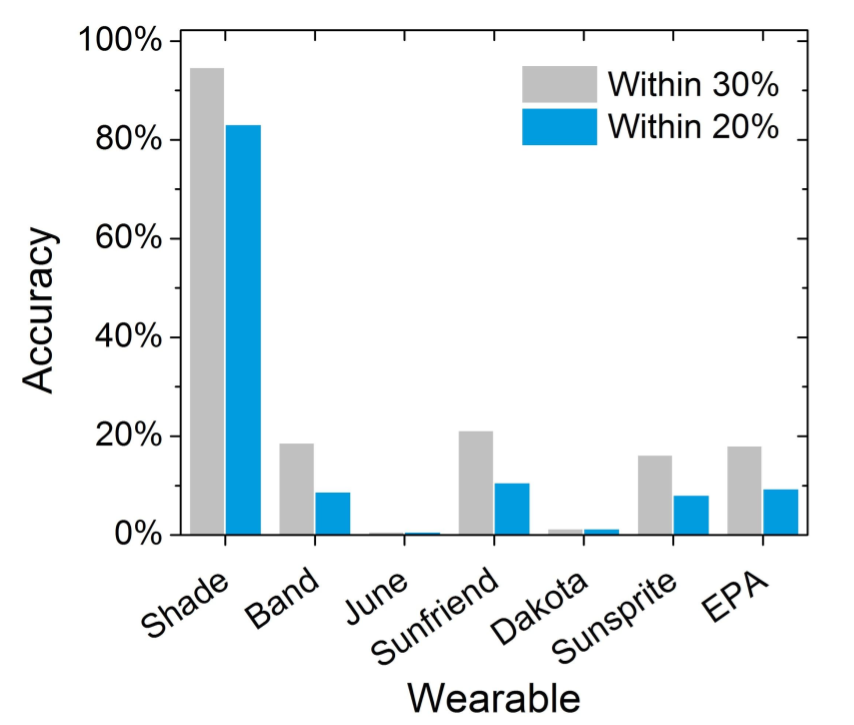
\includegraphics[width=.6\textwidth]{UVSensors.png}}
\caption{Accuracy of commercial UV sensors, with the X1-4 UVE radiometer used as
reference}
\label{fig:uv_sensors}
\end{figure}

The Shade mobile application accounts for people's differences in UV limits and
sensitivity, taking into account their skin type, medication, age and history of
prior sunburns, as even with people with the same skin type often have large
differences in UV exposure sensitivity~\cite{wearshade_sensitivity}. Shade's application addresses
this problem by recommending UV limits during the initial on-boarding screen of
the application, seen in~\cite[\fig{fig:shade_onboarding}]{wearshade_sensitivity}. The application also
allows tracking of the percentage of daily limit reached, along with the real
time UV Index, as seen in~\cite[\fig{fig:shade_measurement}]{wearshade_store}. The full sized
images can be found in \app{app:shade_screenshots}.

% TODO
\begin{figure}[h]
\centering
\begin{minipage}{.5\textwidth}
\centering
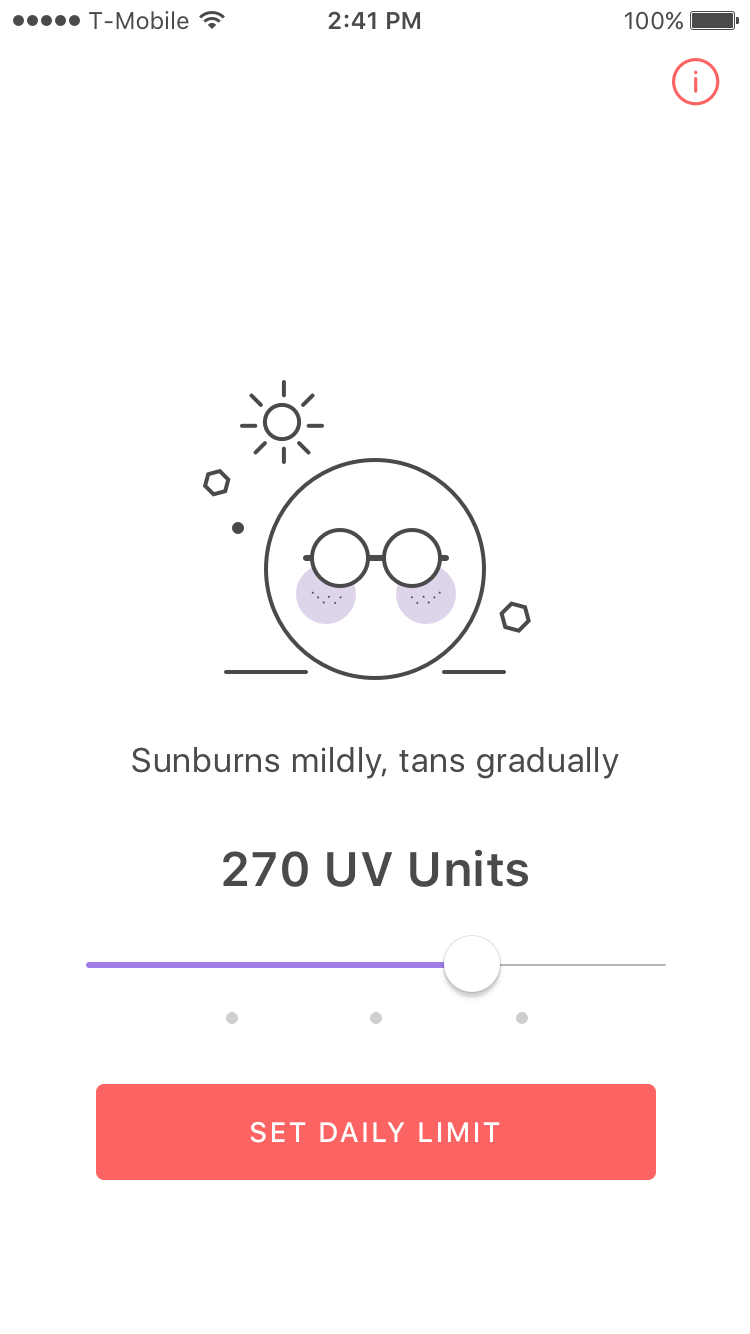
\includegraphics[height=\linewidth]{ShadeOnboarding.png}
\caption{Screenshot of on-boarding screen in Shade's iOS application}
\label{fig:shade_onboarding}
\end{minipage}\begin{minipage}{.5\textwidth}
\centering
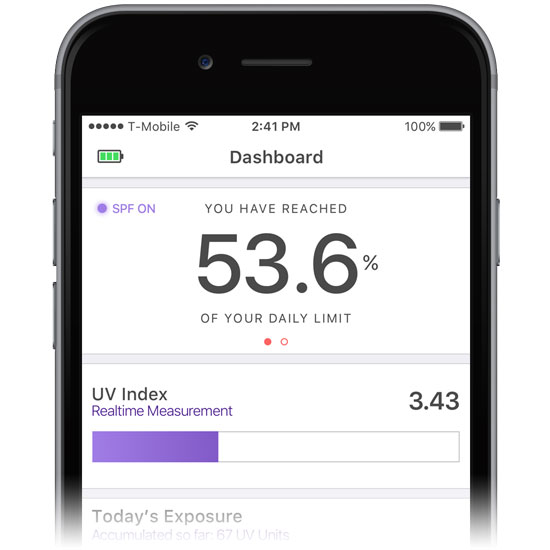
\includegraphics[height=\linewidth]{ShadeMeasurement.jpg}
\caption{Screenshot of measurement screen in Shade's iOS application}
\label{fig:shade_measurement}
\end{minipage}
\end{figure}

The Shade sensor provides an easy to use, accurate, splash-proof UV measurement
device, with a rechargeable battery via a micro USB cable, for a price of
US\$299~\cite{wearshade_store}.

\subsection{QSun}

The QSun wearable is a Federal Communications Commission (FCC) (USA) approved UV
exposure tracker, aiming to reduce the risk of sunburn and skin damage, by
monitoring UV exposure levels, along with vitamin D levels~\cite{qsun_intro}. The 2018
model of the QSun wearable, along with the QSun smartphone application,
provides:

\begin{itemize}
	\item tracking of sun exposure;
	\item tracking of vitamin D production;
	\item personalised tips based on the real time UV Index;
	\item sunscreen amount estimation;
	\item sunscreen reminders;
	\item daily UV Index forecast;
	\item UV Index map;
	\item skin health analysis; and
	\item sun exposure history.
\end{itemize}

The sunscreen recommendation, real time UV Index, and sunscreen amount
estimation screens of the application can be seen
in~\cite[\fig{fig:qsun_screenshots}]{qsun_features}, with a full version in
\app{app:qsun_screenshots}.

\begin{figure}[h]
\centerline{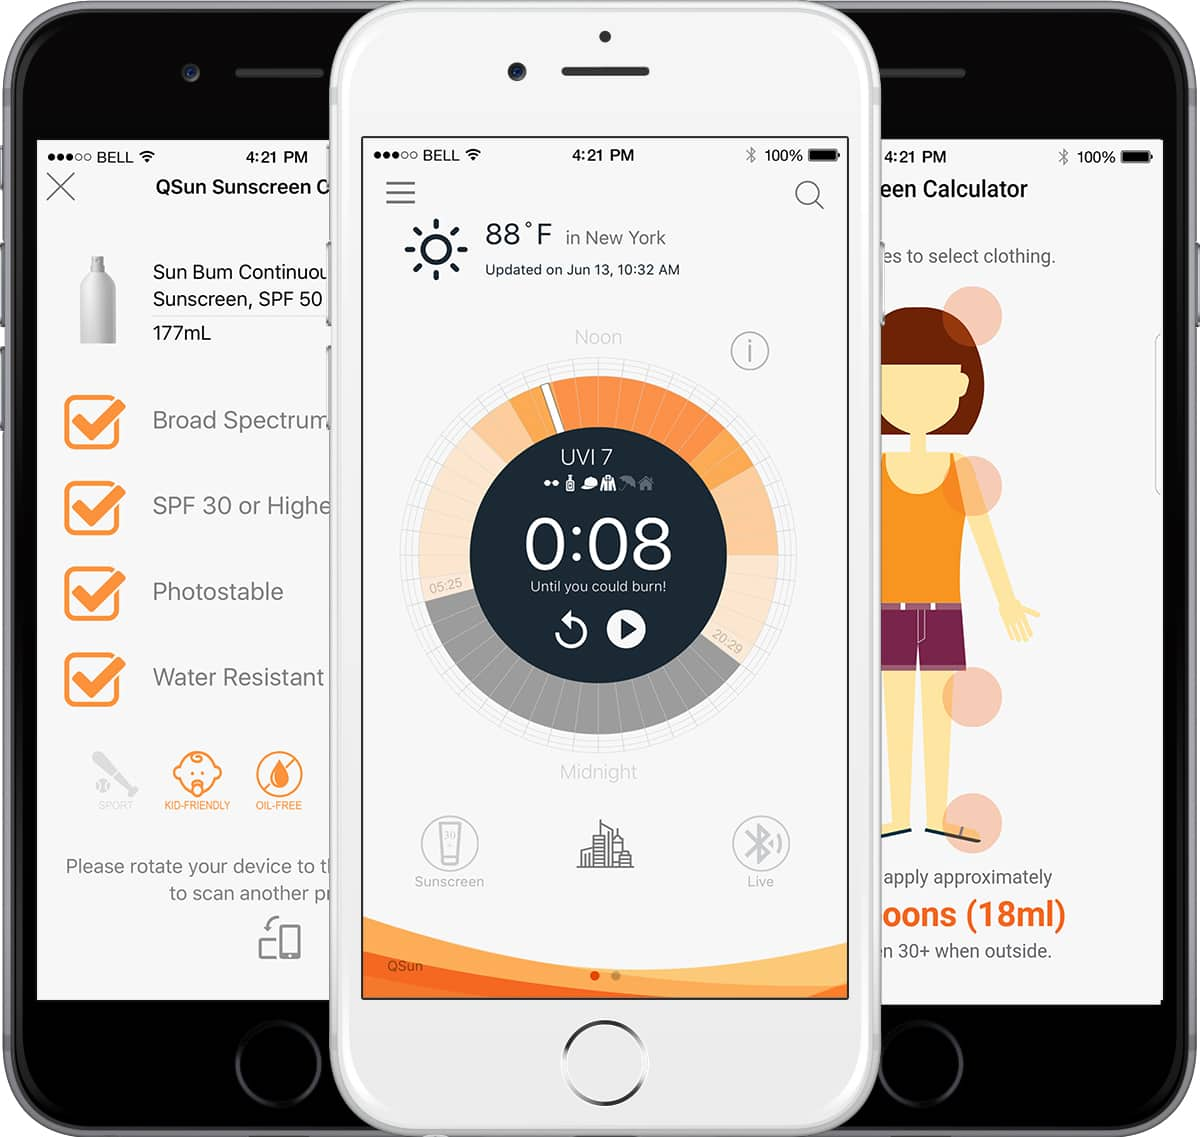
\includegraphics[width=.5\textwidth]{QSunApp.jpg}}
\caption{Screenshots of the sunscreen recommendations (left), real time UV Index
(middle), and sunscreen amount estimation (right) screens in QSun's iOS
application}
\label{fig:qsun_screenshots}
\end{figure}

QSun claims the application communicates and syncs with the wearable via BLE,
with an accurate UVA/UVB index reading within $\pm0.5$ UVI. QSun seems to measure both UVA and UVB, similar to Shade in
\tab{tab:uv_sensors}. The QSun website~\cite{qsun_features} also indicates that the
wearable is splash proof, and has a long battery life, with a replaceable
coin-cell battery (CR2032). The wearable has a 256 kb flash memory, which is
capable of saving 45 days of detailed data.

The device has an optimum operating temperature of -30\degs C to +55\degs C, and a retail price of US\$149.

\cleardoublepage

\chapter{Methodology and Design}

\section{Product Design}

\subsection{Sensor and Data Acquisition}
The Smart Beach Mat thesis project will use a single UV Index sensor; the
Adafruit SI1145.

However, this sensor does not directly measure UVA and UVB
radiation waves; it does not contain a UV sensing element. However, it has a
calibrated light sensing algorithm which estimates the UV Index based on visible
and infra red light~\cite[\fig{fig:adafruit_si1145}]{adafruit_si1145}.

The SI1145 is a low
powered sensor, and can be configured to include features such as proximity
sensing, and ambient light sensing. To sense the visible and IR light, it is
integrated with high-sensitivity visible and infrared photodiodes~\cite{adafruit_si1145_datasheet}. It
offers outstanding performance under a wide range of light sources, such as
sunlight, and even under dark glass covers. It also offers data transmission
using I2C Serial communications, with up to a 3.4 Mb/s transfer rate. This
sensor is also capable of operating from 1.71 V to 3.6 V within -40\degs C and +85\degs C
temperatures~\cite{adafruit_si1145_datasheet}.

This high upper limit on the operating temperature makes
it suitable for keeping under warm conditions for longer periods of time, such
as direct sunlight, which complements its main use case.

\begin{figure}[h]
\centerline{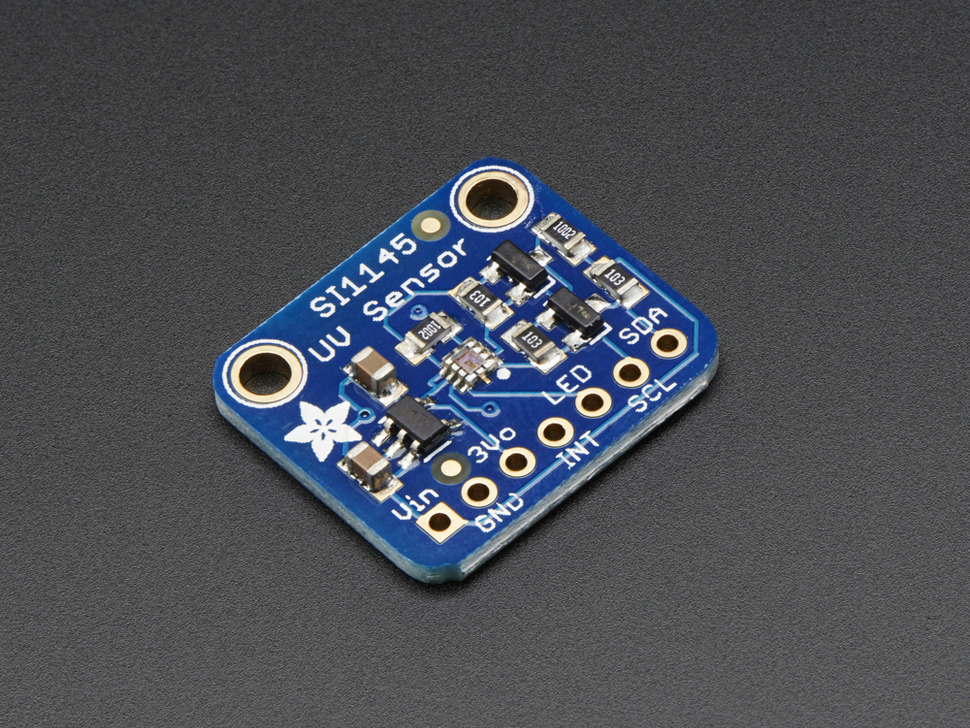
\includegraphics[width=.5\textwidth]{AdafruitSI1145.jpg}}
\caption{The Adafruit SI1145 visible light and IR sensor}
\label{fig:adafruit_si1145}
\end{figure}

\subsection{Microcontroller}

The data from the SI1145 sensor will be transmitted an ESP32 micro-controller.
This micro-controller is responsible for receiving the data through the sensors
I2C interface, and forwarding this data to a mobile application using the
micro-controller's BLE interface. The ESP32 is also capable of WiFi and BLE
communication. Two versions of the ESP32 micro-controller will be used throughout
the development of the project:

\begin{itemize}
	\item ESP32 Thing development board~\cite[\fig{fig:sparkfun_thing}]{sparkfun_thing}
	\begin{itemize}
		\item a developer friendly development board, with
		components such as micro-USB ports, LEDs, and through-hole pins included. This
		will be used for prototyping the initial version of the project, as it simplifies
		the development process.
	\end{itemize}
	\item ESP32 Wroom chip~\cite[\fig{fig:sparkfun_wroom}]{sparkfun_wroom}
	\begin{itemize}
		\item a production-ready, minified version of the ESP32 Thing
		development board. This is only the chip, and therefore does not contain any
		additional components, such as LEDs, or USB ports.
	\end{itemize}
\end{itemize}

\begin{figure}[h]
\centerline{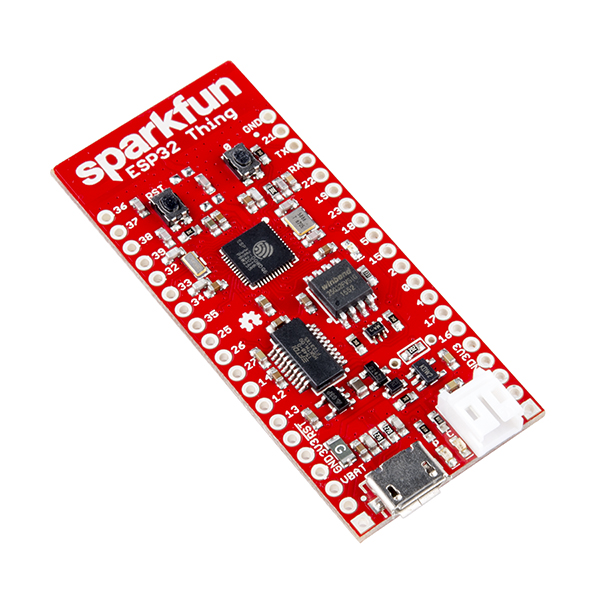
\includegraphics[width=.5\textwidth]{ESP32Thing.jpg}}
\caption{The ESP32 Thing development board}
\label{fig:sparkfun_thing}
\end{figure}

\begin{figure}[h]
\centerline{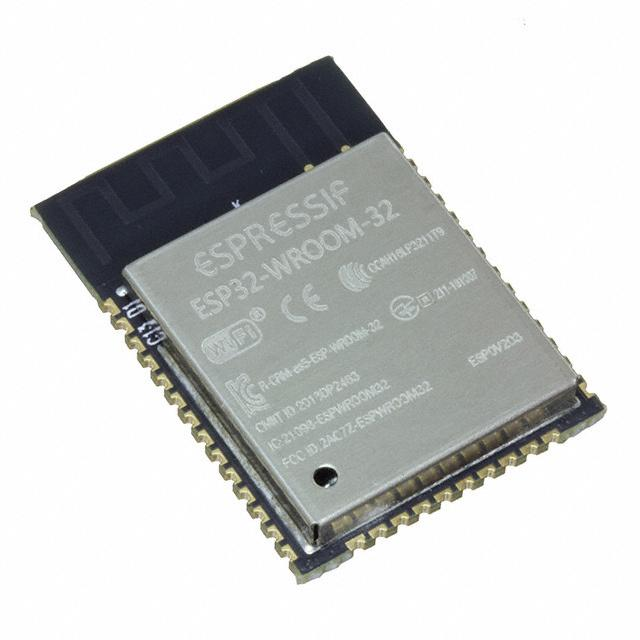
\includegraphics[width=.5\textwidth]{ESP32Wroom.jpg}}
\caption{The ESP32 WROOM microcontroller}
\label{fig:sparkfun_wroom}
\end{figure}

Although two different versions of the ESP32 will be used throughout development,
their core functionality remains the same. The ESP32 runs on 2.2--3.6 V, and is capable of withstanding
temperatures ranging from -40\degs C to +150\degs C; However, the recommended operating
temperature is to be between -40\degs C to +85\degs C~\cite{sparkfun_wroom_datasheet}.
This makes it extremely suitable
for exposure to higher temperatures, however, further mitigation will be required
in order to make it suitable for operating in direct sunlight for longer periods,
as discussed in \secn{secn:project_plan}.

\subsection{Power Supply}
\label{secn:power_supply}

One of the main drawbacks of the compared models in \secn{secn:prior_art} was
their battery life, and modes of battery recharging. These included recharging
the UV sensor through a micro-USB cable, or replacing a cell-coin battery. None
of these methods take advantage of the energy provided from the sun.

This thesis
project will rely on solar power to power the ESP32, along with a rechargeable
battery. However, the battery will be recharged by the solar panel, therefore it
will not need manual recharging. The solar cell will both power the ESP32 and
charge the battery while in sunlight. If there is low to no sunlight, the ESP32
will rely on the battery for power. This method of providing energy also allows
full encapsulation of the device, without relying on any external ports, this
allowing the device to be completely waterproof.

Since the Adafruit SI1145 UV sensor can take
anywhere between 3--5 voltV, and the ESP32 takes 2.2--3.6 V, we'll need a
battery that can provide anywhere from 3--3.6 V, so it can successfully
power both the UV sensor and the ESP32. A lithium-ion battery will be used for
this purpose, due to its great energy density, close to three times that of
Nickel- Cadmium batteries. Lithium is the lightest known metal, providing the
largest energy density per weight~\cite[\fig{fig:energy_density}]{lin}.

\begin{figure}[h]
\centerline{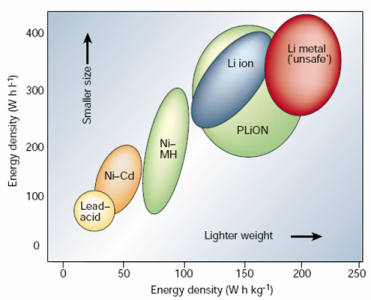
\includegraphics[width=.5\textwidth]{EnergyDensity.png}}
\caption{Energy density of batteries by size and weight}
\label{fig:energy_density}
\end{figure}

The solar
power will work by charging the battery, and the related components (ESP32, UV
sensor) will draw power from the battery. In order for the solar power to safely
and efficiently power the battery, a solar charge controller will be needed.
This will regulate the voltage and current, keep batteries from overcharging,
and ensure no current flows back to the solar panel, hence draining the
battery~\cite{solar_electric}. The basic setup of a solar charge controller can be seen in
\fig{fig:solar_charge_controller}.

\begin{figure}[h]
\centerline{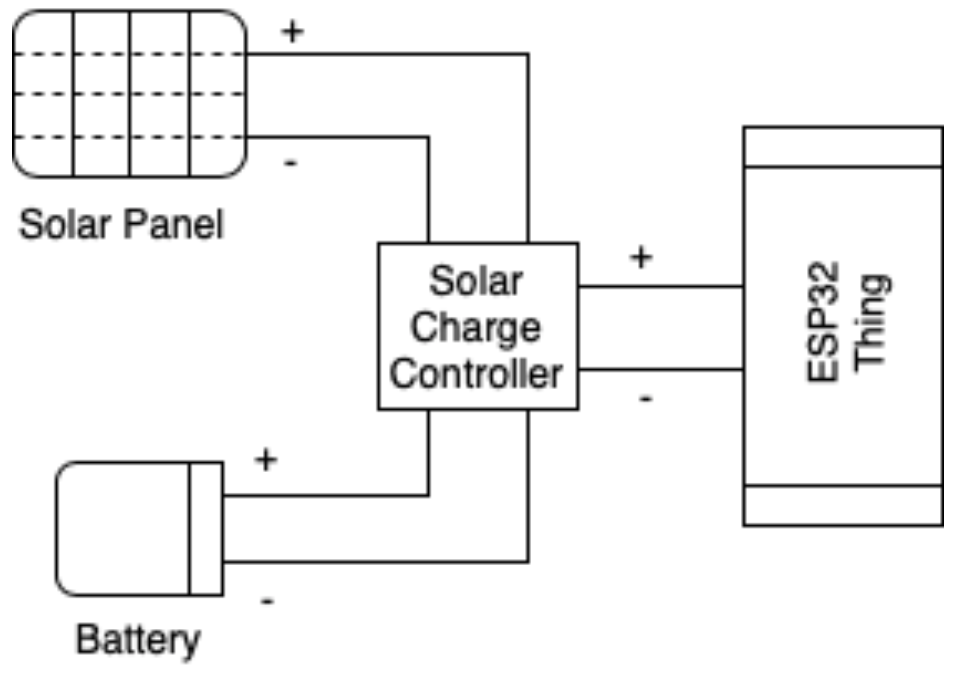
\includegraphics[width=.5\textwidth]{SolarChargeController.png}}
\caption{Solar charge controller setup with ESP32}
\label{fig:solar_charge_controller}
\end{figure}

\subsection{System Architecture}

The system architecture will be made up of the combinations of communication
methods outlined previously. A system architecture diagram of the used protocols
and communication methods can be seen in \fig{fig:system_architecture}.

\begin{figure}[h]
\centerline{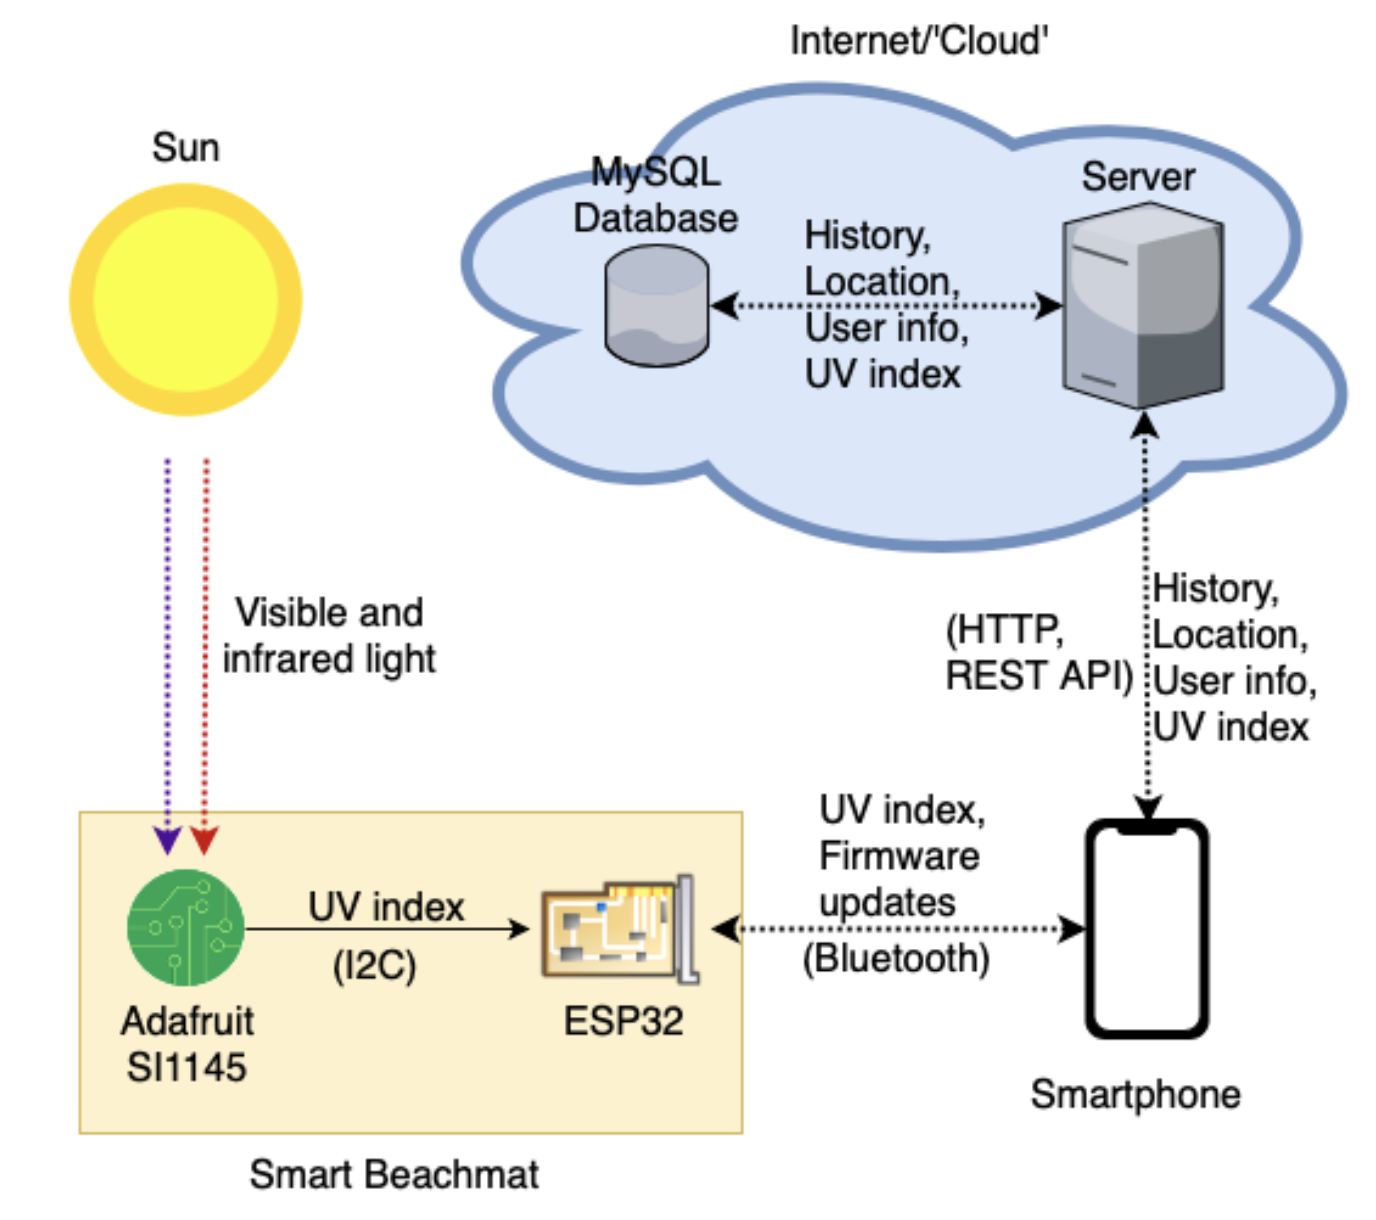
\includegraphics[width=.8\textwidth]{SystemArchitecture.png}}
\caption{System architecture diagram}
\label{fig:system_architecture}
\end{figure}

\subsubsection{I2C}

When the Adafruit SI1145 reads the UV Index based on the visible and infrared
light emitted from the sun, it will need to communicate the read UV Index to the
ESP32. This will be done through the I2C communication method.

I2C is a
synchronous, serial, wired communication method, intended for short range
communication between master and slave devices~\cite{sparkfun}. In this case, our
master node is the ESP32, as it generates the clock and initiates communication
with the slave. Our slave node is the Adafruit SI1145 sensor, which receives the
clock and responds to the ESP32 when instructed.

\subsubsection{BLE}

BLE will be used to communicate the received UV Indexes from the ESP32 to the
smartphone application, as well as the battery level of the ESP32.

In order for
the two devices to communicate, they must first establish the communication by
advertising. The device performing the advertising is known as the
peripheral~\cite{woolley_2016}, and in this case, is the ESP32. The device doing
the scanning (searching) for advertisements is known as the central device~\cite{woolley_2016}, and
will be the smartphone in this case. When performing the advertising, the
peripheral device broadcasts advertising packets, which can contain information about
that device, such as its name, or service UUID. This way, when the central
device is scanning for peripherals, it can filter out the unwanted
devices~\cite{argenox}.

BLE will also be used to send firmware updates from the smartphone to the ESP32
in the background, without the user noticing. This
is done so the firmware of the ESP32 can be updated with features such as
security improvements, without the user having to manually reprogram the device
for each update.

A BLE peripheral has a Generic Attributes Profile (GATT), which
specify the structure and format of the data exchanged, defining basic elements
such as services or characteristics~\cite{martinbl}. A BLE peripheral has one or more
services, and each of those services has one or more characteristics. A service
is a collection of data and behaviours which define a particular function or
feature of the device~\cite{martinbl}. These services are standardised by the
Bluetooth Special Interest Group (SIG). The services used for this project will
be the \verb|Battery Service| and \verb|Environmental Sensing| service, with service UUIDs
\verb|0x180F| and \verb|0x181A| respectively~\cite{bluetooth_gatt}.

A characteristic is a value used in a
service with information about the value's format — how the value is
represented and accessed~\cite{martinbl}. Characteristics are also standardised by
Bluetooth SIG. Within the \verb|Battery Service|, the \verb|Battery Level| characteristic will
be used in order to transmit the ESP32's battery level~\cite{bluetooth_battery_service}. Within the
\verb|Environmental Sensing| service, the \verb|UV Index| characteristic will be used to
represent the UV Indexes read from the sensor~\cite{bluetooth_environmental_sensing}.

Once the advertising
has been done and the devices are connected, the peripheral will send periodic
notifications to the central device. Sending notifications means the phone
doesn't have to keep reading the value from the peripheral, as it will be
notified by the peripheral when the data is sent. Consequently, the ESP32 can read
the UV data periodically, and notify the smarthphone.

\subsubsection{HTTP}

HTTP will be made use of in order to communicate data between the smartphone and
the web server and MySQL database. More specifically, a representational
state transfer (REST) software architectural
style will be used to define the exchanged messages. Although not standardised, the
REST API approach encourages certain request and response formats and behaviours,
to allow for greater flexibility and robustness of HTTP requests~\cite{rest_api}
(see \secn{secn:rest_api} for more information).

For example, when a user registers with the
smartphone application, a user will need to be created in the database on the
cloud, so the user's data can be saved and accessed. The smartphone application
will also send other data to the server, such as the UV Index history of the
user, and the location of the user's phone. The location would be needed in
order to collect location-based UV information, which may be made publicly
available to third-parties, such as the government, to provide and democratize
UV Index values across the country.

The REST API will be created to aid this client-server
communication, and provide a reliable and robust data exchange. The REST API is
a standardised software architecture style which defines a set of constraints
and formats to send and receive HTTP requests~\cite{www_consortium}. This standard allows a
reusable and robust way of handling and making HTTP requests in order to perform
create, read, update, and delete (CRUD) operations on the server-side.

\section{Project Plan}
\label{secn:project_plan}

\subsection{Software Development Process}
\label{secn:software_development_process}

The project will be undertaken using the Scrum software development process.
Scrum is an Agile framework, where development on a product is undertaken in
iterated sprints, lasting from 2--4 weeks. Scrum is made up of the following
phases and components~\cite{scrum_intro}:
\begin{itemize}
	\item Product backlog
	\begin{itemize}
		\item The set of product features and requirements specified by the
		client (product owner).
	\end{itemize}
	\item Sprint backlog
	\begin{itemize}
		\item A subset of the product backlog, specifying which the goals of the
		upcoming sprint, and what features will be implemented in the product
		during that sprint.
	\end{itemize}
	\item Daily scrum
	\begin{itemize}
		\item A stand-up meeting, where each developing team member has a
		discussion every day regarding the progress of the sprint. Teach team
		member will share and discuss their progress since the last stand-up,
		what they're planning to work on up until the following stand-up, and
		any blocks or issues they're facing.
	\end{itemize}
	\item Sprint review
	\begin{itemize}
		\item A meeting with the client reviews the team's progress, and the
		product backlog, making adjustments to the plan by adding or removing
		certain features, to meet the client's needs~\cite{scrum_sprint_review}.
	\end{itemize}
	\item Sprint retrospective
	\begin{itemize}
		\item The sprint retrospective is a reflection amongst developers in
		order to determine what went well during the sprint, what could have
		been done better, and what will be done next. The sprint retrospective
		is done in order to optimise the team's development process~\cite{scrum_sprint_retrospective}.
	\end{itemize}
\end{itemize}

A diagram of the Scrum process can be seen in~\cite[\fig{fig:scrum_framework}]{scrum_intro}.

The development team for this project will consist of a single developer, who
will undertake 2-week sprints, meeting with the client, and making use of each
step of the Scrum framework.

\begin{figure}[h]
\centerline{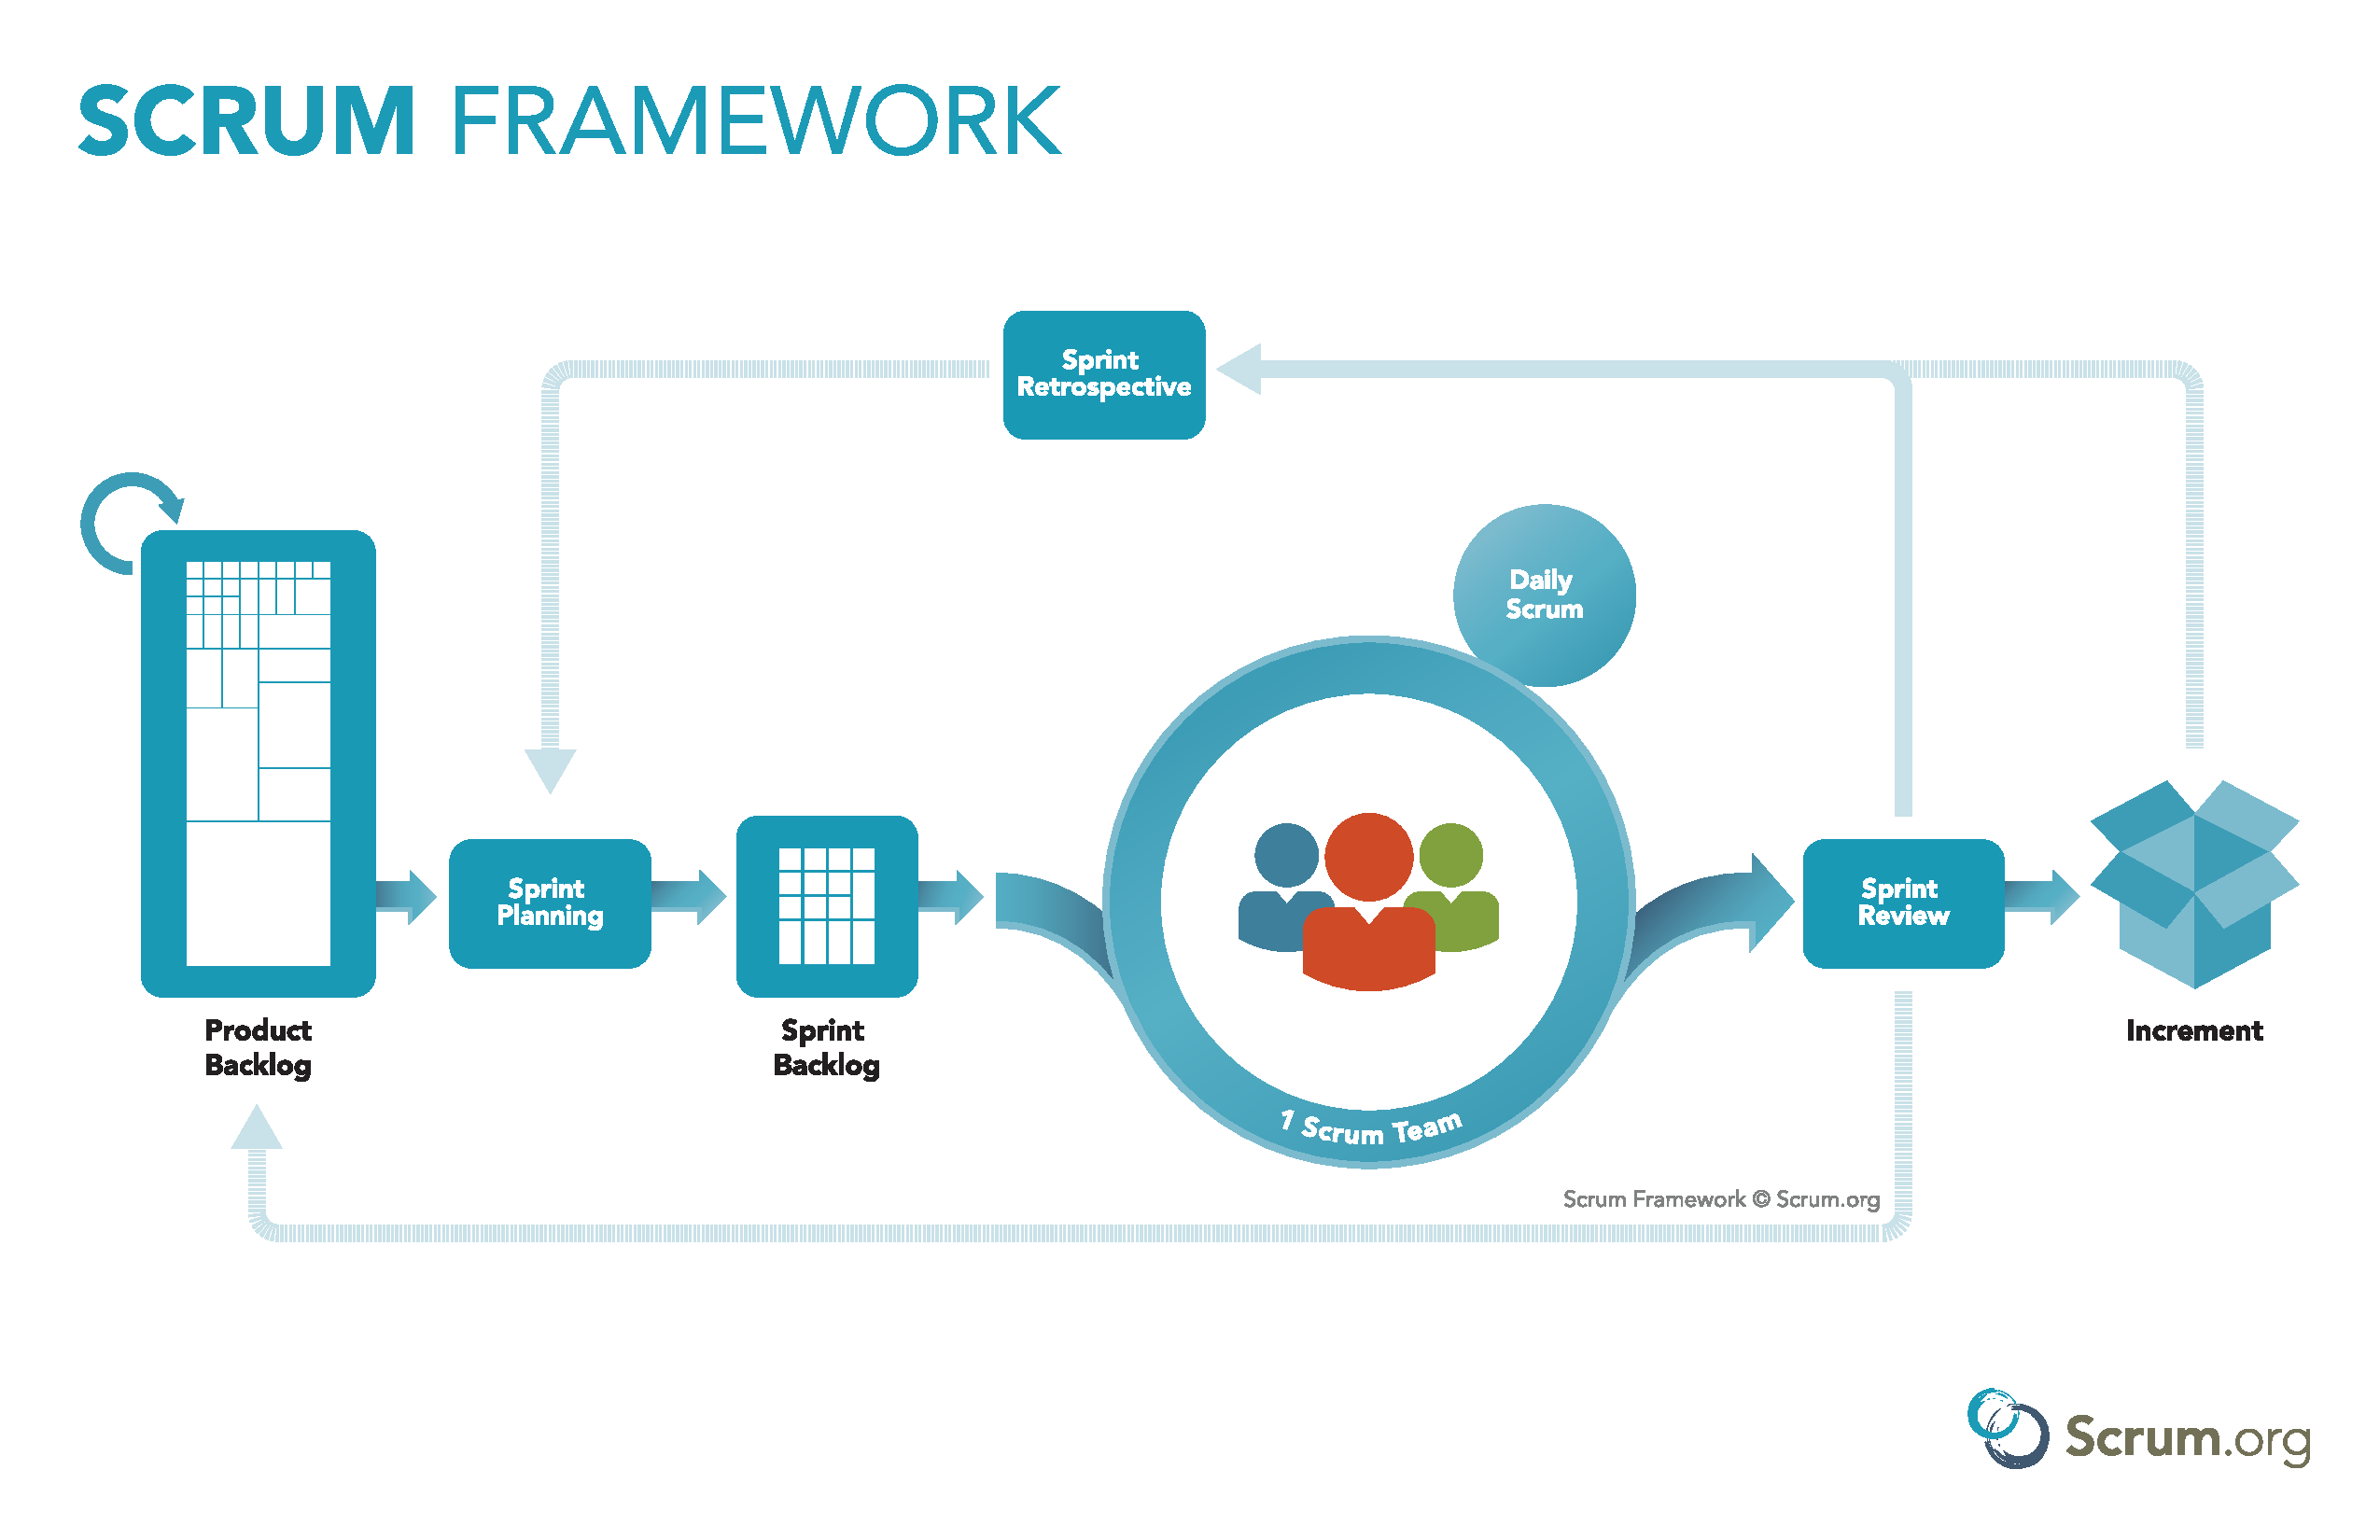
\includegraphics[width=\textwidth]{ScrumFramework.pdf}}
\caption{Scrum framework workflow}
\label{fig:scrum_framework}
\end{figure}

\subsection{Sprint Plan}

The two-semester project will follow the Scrum framework discussed in \secn{secn:software_development_process}.
Hence, the two semesters are broken up into sprints. Since there are 13 weeks per
semester in 2019 at UQ -- resulting in 26 total weeks -- the project has been
broken up into 13 two-week sprints.

The sprint outline can be found in
\tab{tab:sprint_plan}.

\begin{table}[h]
\caption{\sl Sprint plan for 13 sprint sessions.}
\label{tab:sprint_plan}
\begin{center}
\begin{tabular}{|c|l|p{8cm}|}
\hline
Sprint & Period & Tasks \\
\hline
0 & \formatdate{25}{2}{2019} -- \formatdate{10}{3}{2019} &
Research relevant, unfamiliar topics, such as the BLE protocol, and Arduino
development. Finalise high-level architecture design. \\
1 & \formatdate{11}{3}{2019} -- \formatdate{24}{3}{2019} &
Conduct user research. (Surveys and product validation.) \\
2 & \formatdate{25}{3}{2019} -- \formatdate{7}{4}{2019} &
Set up local development environment and Git repository. (Set up local server,
with PHP and MySQL database.) \\
3 & \formatdate{8}{4}{2019} -- \formatdate{21}{4}{2019} &
Design hardware prototype. (Schematic diagram.) \\
\hline
\multicolumn{3}{|c|}{Mid-semester break}\\
\hline
4 & \formatdate{29}{4}{2019} -- \formatdate{12}{5}{2019} &
Develop and test hardware prototype. (Test UV readings and BLE communication.) \\
5 & \formatdate{13}{5}{2019} -- \formatdate{26}{5}{2019} &
Design database schema. (ER diagram design.) \\
6 & \formatdate{27}{5}{2019} -- \formatdate{9}{6}{2019} &
Set up database according to schema. (MySQL development.) \\
\hline
\multicolumn{3}{|c|}{Semester break}\\
\hline
7 & \formatdate{22}{7}{2019} -- \formatdate{4}{8}{2019} &
Design REST API. (API endpoints.) \\
8 & \formatdate{5}{8}{2019} -- \formatdate{18}{8}{2019} &
Develop and test REST API. (PHP development.) \\
9 & \formatdate{19}{8}{2019} -- \formatdate{1}{9}{2019} &
Prototype smartphone application. (Low- and high-fidelity prototypes.) \\
10 & \formatdate{2}{9}{2019} -- \formatdate{15}{9}{2019} &
Develop smartphone application. (Flutter development.) \\
11 & \formatdate{16}{9}{2019} -- \formatdate{29}{9}{2019} &
Design and develop final hardware. (PCB design, soldering, casing.) \\
\hline
\multicolumn{3}{|c|}{Mid-semester break}\\
\hline
12 & \formatdate{7}{10}{2019} -- \formatdate{18}{10}{2019} &
Migrate local development environment to public cloud. \\
\hline
\end{tabular}
\end{center}
\end{table}

\subsection{Code Management}

In order to manage the code for the firmware, mobile application, and server,
the Git version control will be used. This will ensure that the source code of
all components is stored on a central Git server, accessible from anywhere. This
will also make it easy to manage code, test out new features, and roll back to
certain commits, given an unwanted change. This will ensure the code is safe and
less prone to cause damage from mistakes such as accidentally breaking code,
providing flexibility in development.

% \bigskip

% \textbf{Approach and execution (45\%):} The thesis should clearly set out the
% approach of the thesis work as an outgrowth of the background research,
% including an evaluation of alternative approaches. The approach should clearly
% state the goals of applying methods, how it resolves the stated hypothesis
% and/or problems, and how the goals will be achieved in a systematic fashion. The
% approach should show innovation and creativity. The execution of the approach
% should demonstrate systematic problem solving with balanced theory and practical
% considerations. You should further demonstrate the ability to respond
% appropriately to problems that arise during the course of the project. The
% documentation should highlight your ability to use your knowledge in different
% contexts, and your ability to acquire and generate new knowledge. The project
% results are complete and comprehensively presented and analysed. In general, the
% execution of the project (as reported in the thesis) should give justice to a
% substantial work effort.

\cleardoublepage

\chapter{Results and Discussion}

% Execution: What and how much you've done, how you've executed the approach --- showing problem solving, indicates substantial work effort.

% The execution indicates a substantial work effort, and shows the application of knowledge gained from background research. The project results are complete and comprehensively presented and analysed.

% \bigskip

% In any case, you will probably need to include tabulated results.
% \tab{tf2} illustrates the use of various \LaTeX\ environments to
% include a computer printout (plain text file) in a document.  The
% \texttt{verbatim} environment, which encloses the formatted text, is
% also useful for program listings.

% \begin{table}\renewcommand{\baselinestretch}{1.0}
% \caption{\sl Fraction of air volume involved in heat exchange for
% second mode (right column) vs.\ filling factor (left column).  The
% plain-text headings represent $f$, $m$, $\mu_2$ and $f_2$.}
% \label{tf2}

% \begin{center}
% \begin{minipage}[c]{2.85in}\small\normalsize
% \begin{verbatim}

%  f(%)     m         mu2     f2(%)

%  0.016   80.00    0.05400   4.874
%  0.031   56.57    0.07732   5.438
%  0.062   40.00    0.11103   6.125
%  0.125   28.28    0.16001   6.970
%  0.250   20.00    0.23175   8.020
%  0.500   14.14    0.33799   9.329
%  1.000   10.00    0.49789  10.967
%  2.000    7.07    0.74444  13.008
%  4.000    5.00    1.13919  15.525
%  8.000    3.54    1.81095  18.568

% 19.237    2.28    3.61958  23.174
% 37.180    1.64    7.28635  27.094
% 57.392    1.32   14.63631  29.813
% 74.316    1.16   29.35160  31.453
% 85.734    1.08   58.79364  32.360
% \end{verbatim}
% \end{minipage}
% \end{center}
% \end{table}

% \section{Product Validation}

% Minor product validation has also been undertaken to understand the viability
% and business potential of the product.

% The main form of idea validation was done through questionnaires. Well
% thought-out questionnaires have been designed and distributed. The questionnaire
% can be found in \tab{}, where the results from the questionnaire are also outlined.

% Voluntarily participants were asked the questions after filling out the participation
% consent form, found in \app{}

% This questionnaire was undertaken by 19 participants, a mixture of people on campus,
% friends, and collegues (UQ STUDENTS, FAMILY, OR FRIENDS ONLY).

% \tab{} summarises the answers from the questionnaires.

%Demographics
% Age
% Gender

%Behavioural
% How worried are you about the effects UV has on your skin?
% How aware are you of the negative effects UV has on your skin?
% How often do you check the UV forecast when going outdoors?
% How often do you go to the beach, or go sunbathing?
% When you go, how long do you spend there on average?
% How many people do you go with on average?
% How would you expect to connect to a smart IoT product with your phone?
% % Bluetooth, without a smartphone application
% % Bluetooth, through a smartphone application
% % Wifi hotspot
% Would you be the only person using this application, or would you prefer for it to have be a shared application?
% Would you prefer to keep a history of your UV exposure data so you can look back at it?

%Our idea...

%Demand
% Is this something you'd need?
% How likely would you be to use it if it was free?
% Have you used/do you use any similar products? If so, what don't you like about them?
% Assuming the price of the product was reasonable, how likely would you be to use it?

% Given these findings, it's clear that most people are not worried and are not aware
% of the UV effects on the skin. They'd prefer to keep track of their data, so storing on
% cloud seems like the ideal option. They'd prefer to connect with Bluetooth. Most
% participants go to the beach / sunbathing ??, and are there for ?? hours. On average,
% they go with ?? additional people. ?? of participants check the UV forecasts prior
% to going out.

\section{Development Environment}

In order to keep the work private, and speed up development time, a local development
environment was set up. A number of things had to be taken care of, including
setting up a local server, configuring the server, and installing MySQL.

A local Apache server was set up on a macOS computer to begin development. Since
macOS comes pre-installed with Apache, the server could be started by typing the
following command on the command line:

\begin{lstlisting}[basicstyle=\ttfamily]
$ sudo apachectl start
\end{lstlisting}

After visiting \verb|localhost:80| in the Safari browser, the screen shown in
\fig{fig:apache_works} was seen, confirming the functionality of the Apache server.

\begin{figure}[h]
\centerline{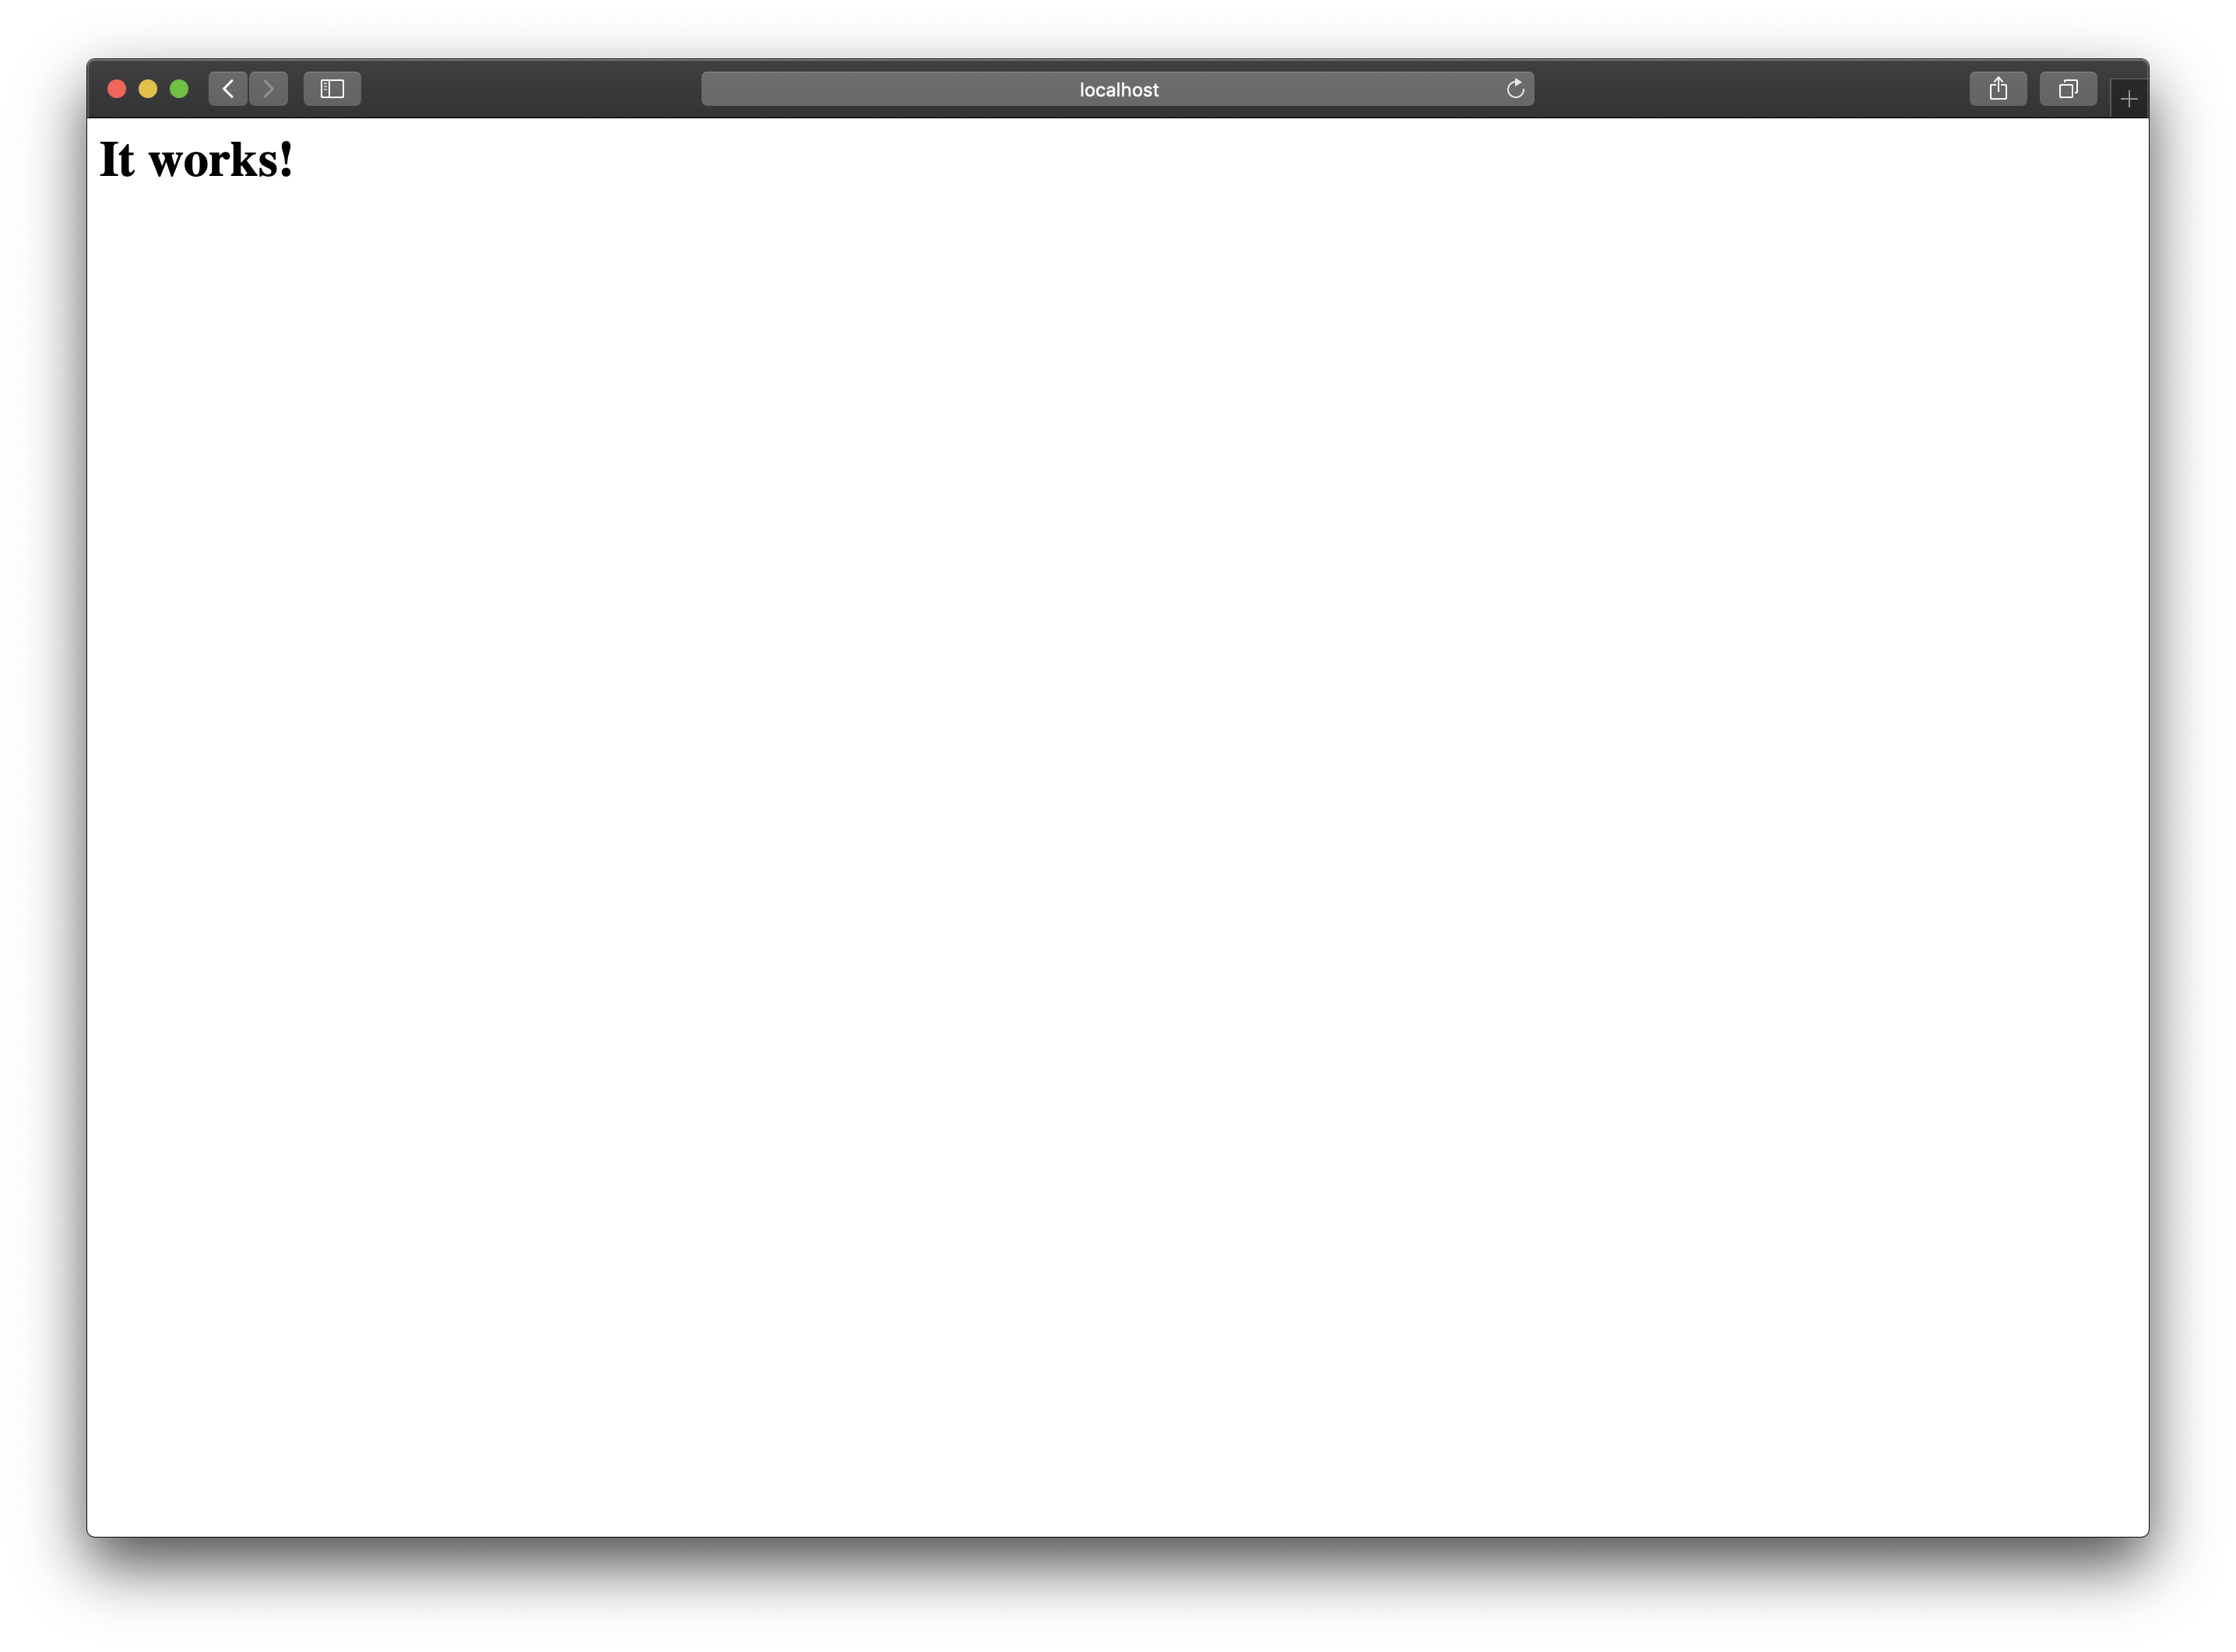
\includegraphics[width=\textwidth]{ApacheItWorks.png}}
\caption{Safari screenshot at localhost:80 after starting local Apache server}
\label{fig:apache_works}
\end{figure}

To organize the workspace however, this wasn't enough. Multiple configurations have
been made to the Apache configuration file (\verb|/etc/apache2/httpd.conf|), to
enable a smoother workflow.

\subsubsection{Change the Document Root Directory}
The document root was changed to a different working directory,
otherwise the web server would look for files in \verb|/Library/WebServer/Documents|.
Changing the working directory also allowed to work in a remote, existing
Git repository.

The following lines had to be added to the Apache configuration file to specify
the new working directory.

\begin{lstlisting}[basicstyle=\ttfamily,breaklines=true]
DocumentRoot "/Users/adamdorogi/Git/myThesis-SmartCampus/SmartBeachmat/smart_beachmat_server"
<Directory "/Users/adamdorogi/Git/myThesis-SmartCampus/SmartBeachmat/smart_beachmat_server">
\end{lstlisting}

\subsubsection{Enable PHP}

Since PHP is the server-side programming language for this project, it had to
be enabled on the local server for development.

To enable PHP, the following line had to be uncommented from the Apache configuration
file, by removing the \verb|#|:

\begin{lstlisting}[basicstyle=\ttfamily,breaklines=true]
#LoadModule php7_module libexec/apache2/libphp7.so
\end{lstlisting}

To test whether PHP was functioning correctly, a simple \verb|index.php| file
was added to the root directory, specified earlier. The contents of the \verb|index.php| are:

\begin{lstlisting}[basicstyle=\ttfamily,breaklines=true,language=PHP]
<?php
echo "Hello ENGG4801!";
phpinfo();
?>
\end{lstlisting}

Visiting \verb|localhost:80| after adding the \verb|index.php| file resulted in
the screen seen in \fig{fig:php_info}.

\begin{figure}[h]
\centerline{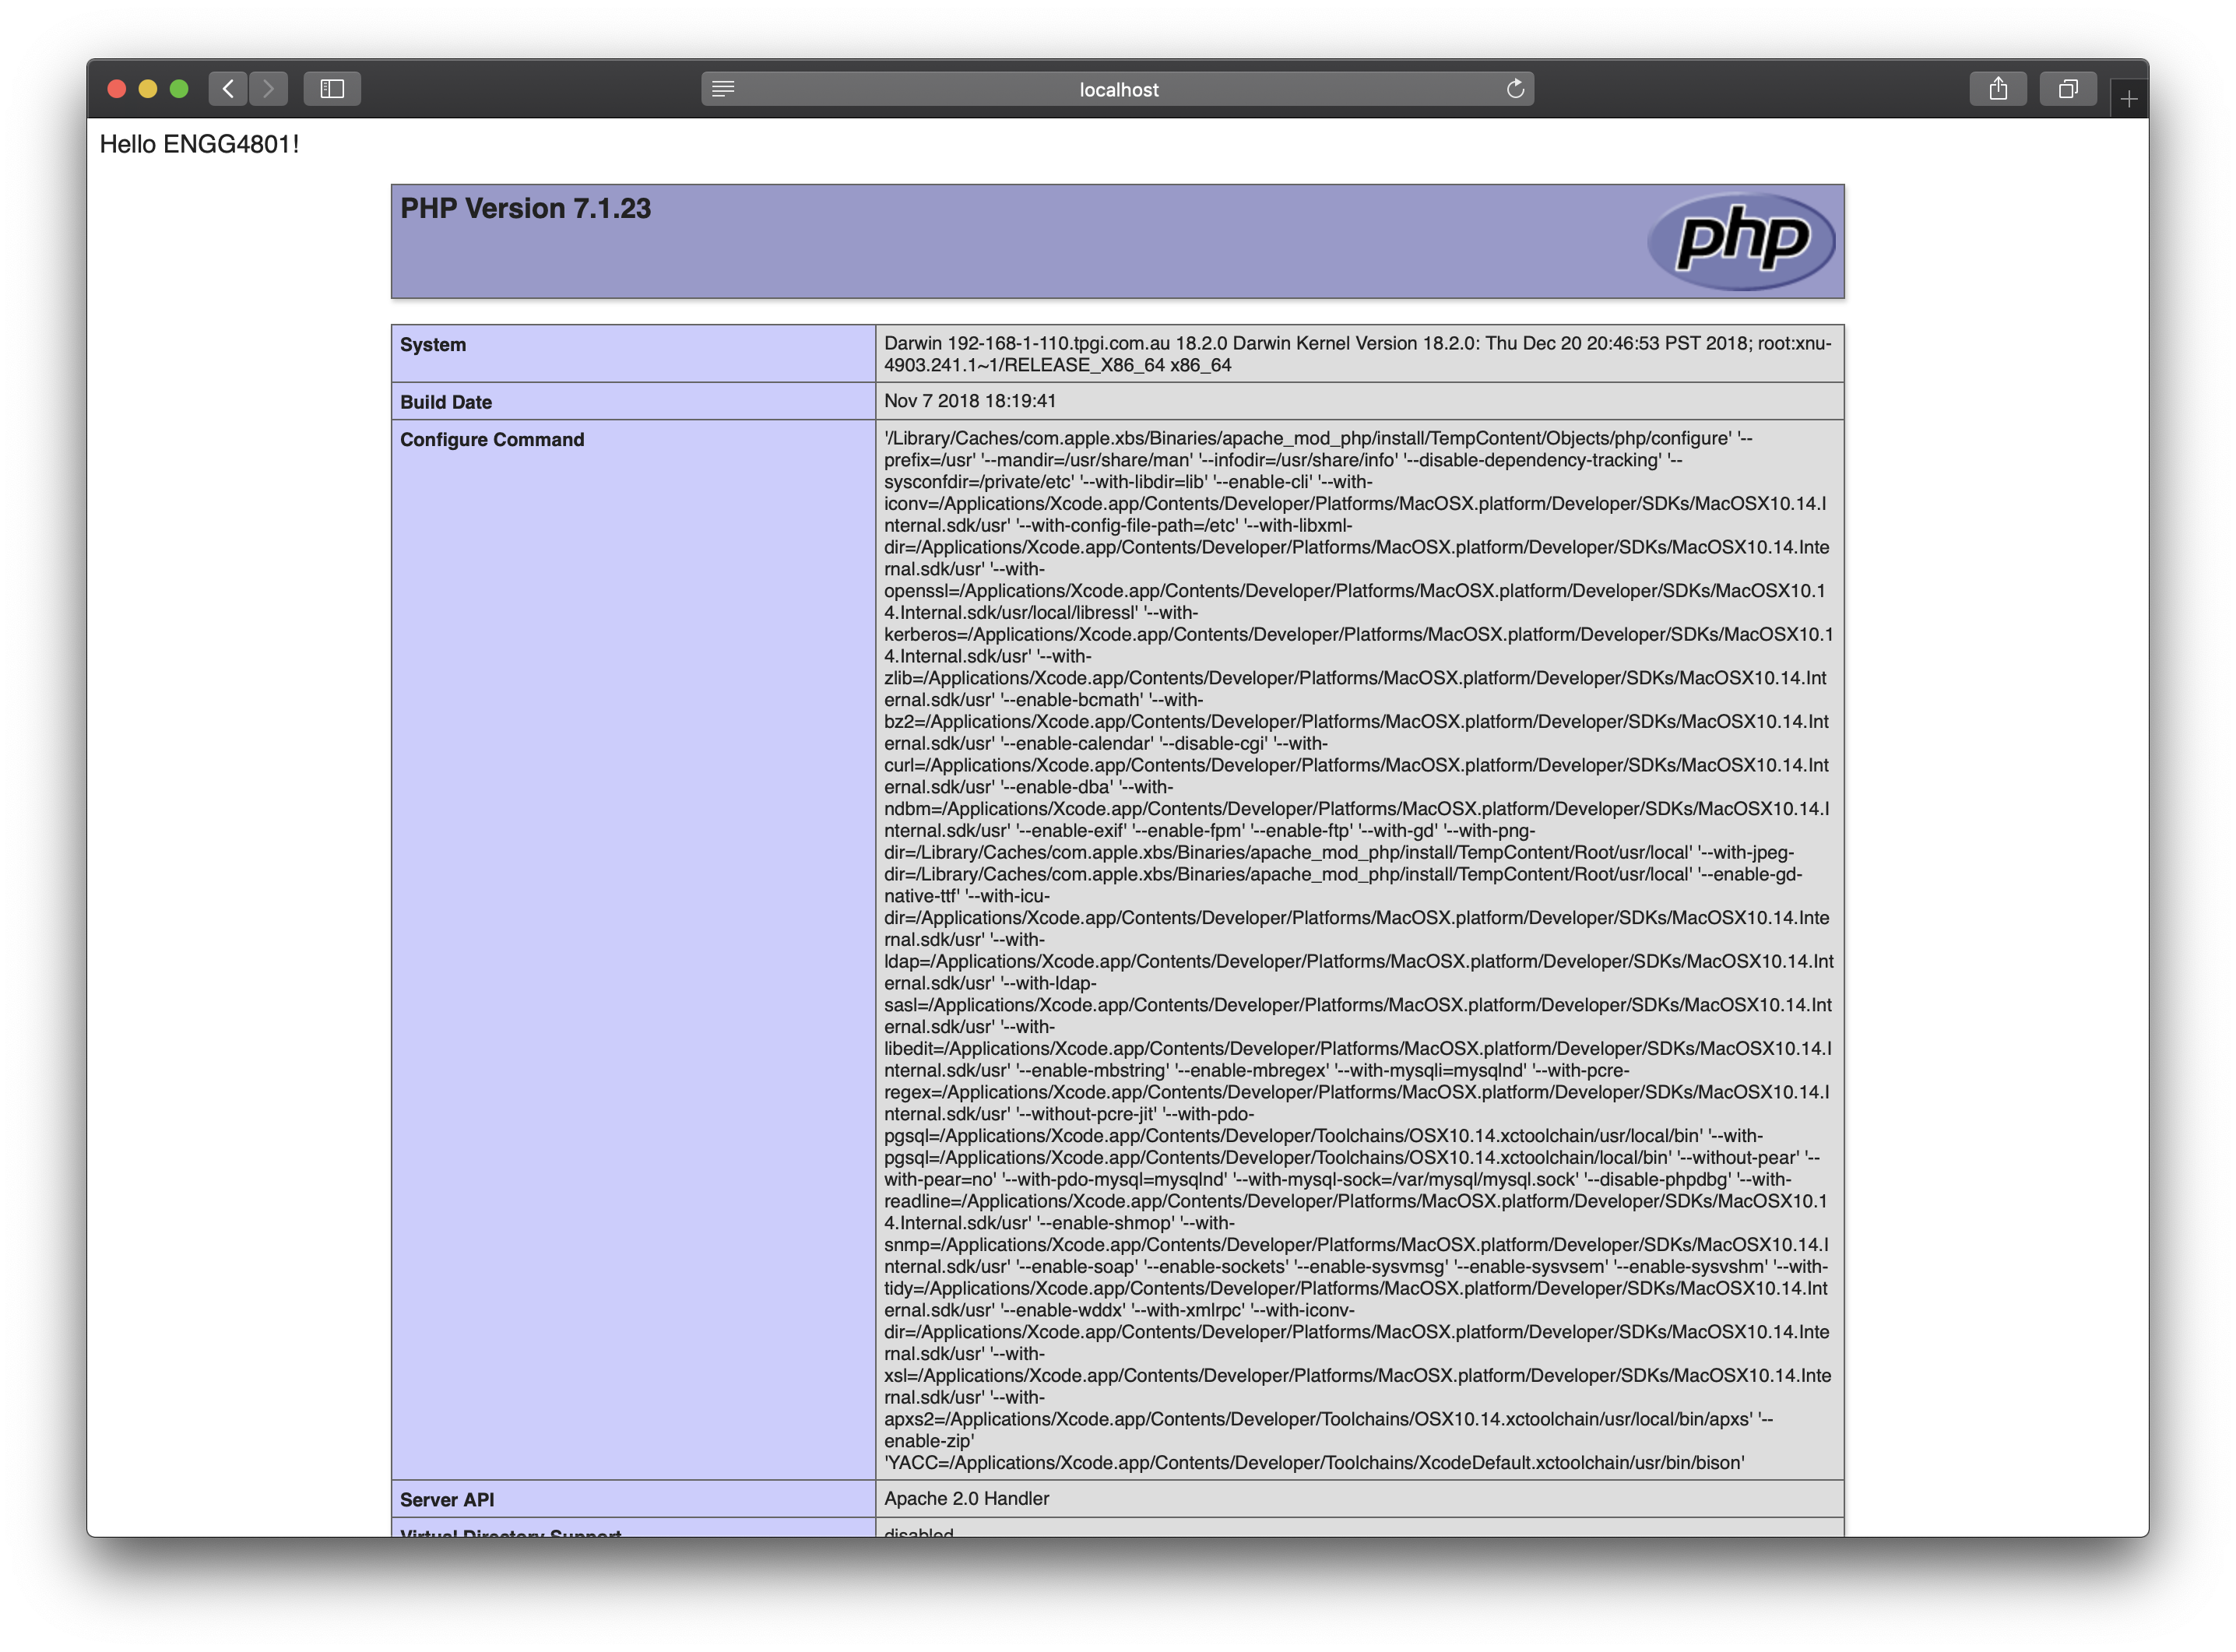
\includegraphics[width=\textwidth]{PHPInfo.png}}
\caption{Safari screenshot at localhost:80 after enabling PHP}
\label{fig:php_info}
\end{figure}

\subsubsection{Installing MySQL}

To install MySQL, it was first downloaded from \verb|mysql.com|, along with
PHPMyAdmin from \verb|phpmyadmin.net| (a graphical management interface for MySQL).

To install PHPMyAdmin, the downloaded \verb|phpMyAdmin| folder had to be moved
to the root folder. For the complete folder structure of the project, see \secn{secn:structure}.

MySQL had to be started through System Preferences, otherwise the following error
would occur when trying to log in to the \verb|phpMyAdmin| interface at \verb|localhost:80/phpMyAdmin|.

\begin{lstlisting}[basicstyle=\ttfamily,breaklines=true]
mysqli_real_connect(): (HY000/2002): No such file or directory
\end{lstlisting}

Another challenge was encountered during installation of MySQL, which was:

\begin{lstlisting}[basicstyle=\ttfamily,breaklines=true]
mysqli_real_connect(): The server requested authentication method unknown to the client [caching_sha2_password]
\end{lstlisting}

After researching the GitHub repository of \verb|phpMyAdmin| however, this issue
could be resolved.

%TODO
% However, after researching github issues, solution was found
% [https://github.com/laradock/laradock/issues/1390] OR [https://github.com/phpmyadmin/phpmyadmin/issues/14220],
% which updates your root database login to use the old password authentication
% method, rather than this new one --- through /usr/local/mysql/bin command

% With these workarounds in place, local dev environment was set up and ready to
% go

\section{Hardware}

\subsection{Prototype}
\label{secn:prototype}

To start developing the hardware prototype, the Araduino IDE was downloaded from
\verb|arduino.cc|. Arduino is a development environment, which is used to program
specific microcontrollers, such as the ESP32 Thing development board.

The ESP32 Thing was plugged in to the computer, and the following Hello World
script~\cite{sparkfun_thing} was programmed onto the device, to ensure everything was working correctly.

\begin{lstlisting}[basicstyle=\ttfamily,breaklines=true,language=c++]
int ledPin = 5;

void setup()
{
    pinMode(ledPin, OUTPUT);
    Serial.begin(115200);
}

void loop()
{
    Serial.println("Hello, world!");
    digitalWrite(ledPin, HIGH);
    delay(500);
    digitalWrite(ledPin, LOW);
    delay(500);
}
\end{lstlisting}

This script blinked the LED on the ESP32 development board every half seconds.
Once the Hello World application has been successfully tested, the Arduino
project was replaced with example code provided by the ESP32 Arduino BLE library~\cite{arduino_ble_write},
called \verb|BLE_write|. The provided code can be seen in \app{code:ble_write}.

This code allows the ESP32 to write to the device it's connected to, once data
is requested. To test this functionality, The BLE communication has been tested
out on an iPhone, with a free application from the AppStore, intended for
Bluetooth testing purposes. Hardcoded values were successfully sent to the
testing application.

Once data was successfully being sent over the BLE communication channel, the
Adafruit SI1145 UV sensor was connected to the ESP32, and the Arduino project
was expanded with the Adafruit's library for the SI1145 UV sensor, downloaded
from~\cite{adafruit_code}. To install the library, the following were done:
\begin{itemize}
	\item Rename the uncompressed folder \verb|Adafruit_SI1145|, ensuring the
	folder still contains \verb|Adafruit_SI1145.cpp| and \verb|Adafruit_SI1145.h|
	\item Place the \verb|Adafruit_SI1145| library folder into the \verb|arduinosketchfolder/libraries/|
	folder. 
	\item Restart the IDE.
\end{itemize}

This library enabled retrieving UV and infrared sensing data from the SI1145,
and the code snippet used to test this functionality can be found
in~\cite[\app{code:si1145test}]{adafruit_code}.

The next step was to communicate the read values over BLE to the testing app.
This was done by simply combining parts of the snippet from both \app{code:ble_write} and \app{code:si1145test}.

However, it was later realised that it wasn't enough to only 'read' values from
the ESP32, but it made more sense to notify the application at certain
intervals.

%TODO
% The next question was, how often do we send UV Index values to the
% app? An experiment has been done to find out:

% READ ALL UV IndexES FOR 24 HOURS

The final code programmed onto the ESP32 can be found in \app{code:final}, and
the final set up of the prototype can be seen in \fig{fig:prototype}

\begin{figure}[h]
\centering\includegraphics[width=0.5\textwidth]{Prototype.jpg}
\caption{Prototype of UV sensing IoT device}
\label{fig:prototype}
\end{figure}

\subsection{Final}

During the development of the device, it was decided that due to time
constraints, the device wasn't going to rely on solar power. Due to the lack of
electrical engineering knowledge, and lack of time for thorough reliable
research. Instead, it was decided that it will rely on Lithium Ion battery only,
as discussed in \secn{secn:power_supply}.

The three main components to make up the device were the ESP32 Wroom, the
Adafruit SI1145 UV sensor, and an additional component not initially planned;
a USB battery charger.

The PCB and the schematic for the device was designed using Altium Studio. The
PCB schematic, designed in Altium Studio can be seen in \fig{fig:schematic_screenshot} and \fig{fig:schematic_pdf}.

\begin{figure}[h]
\centering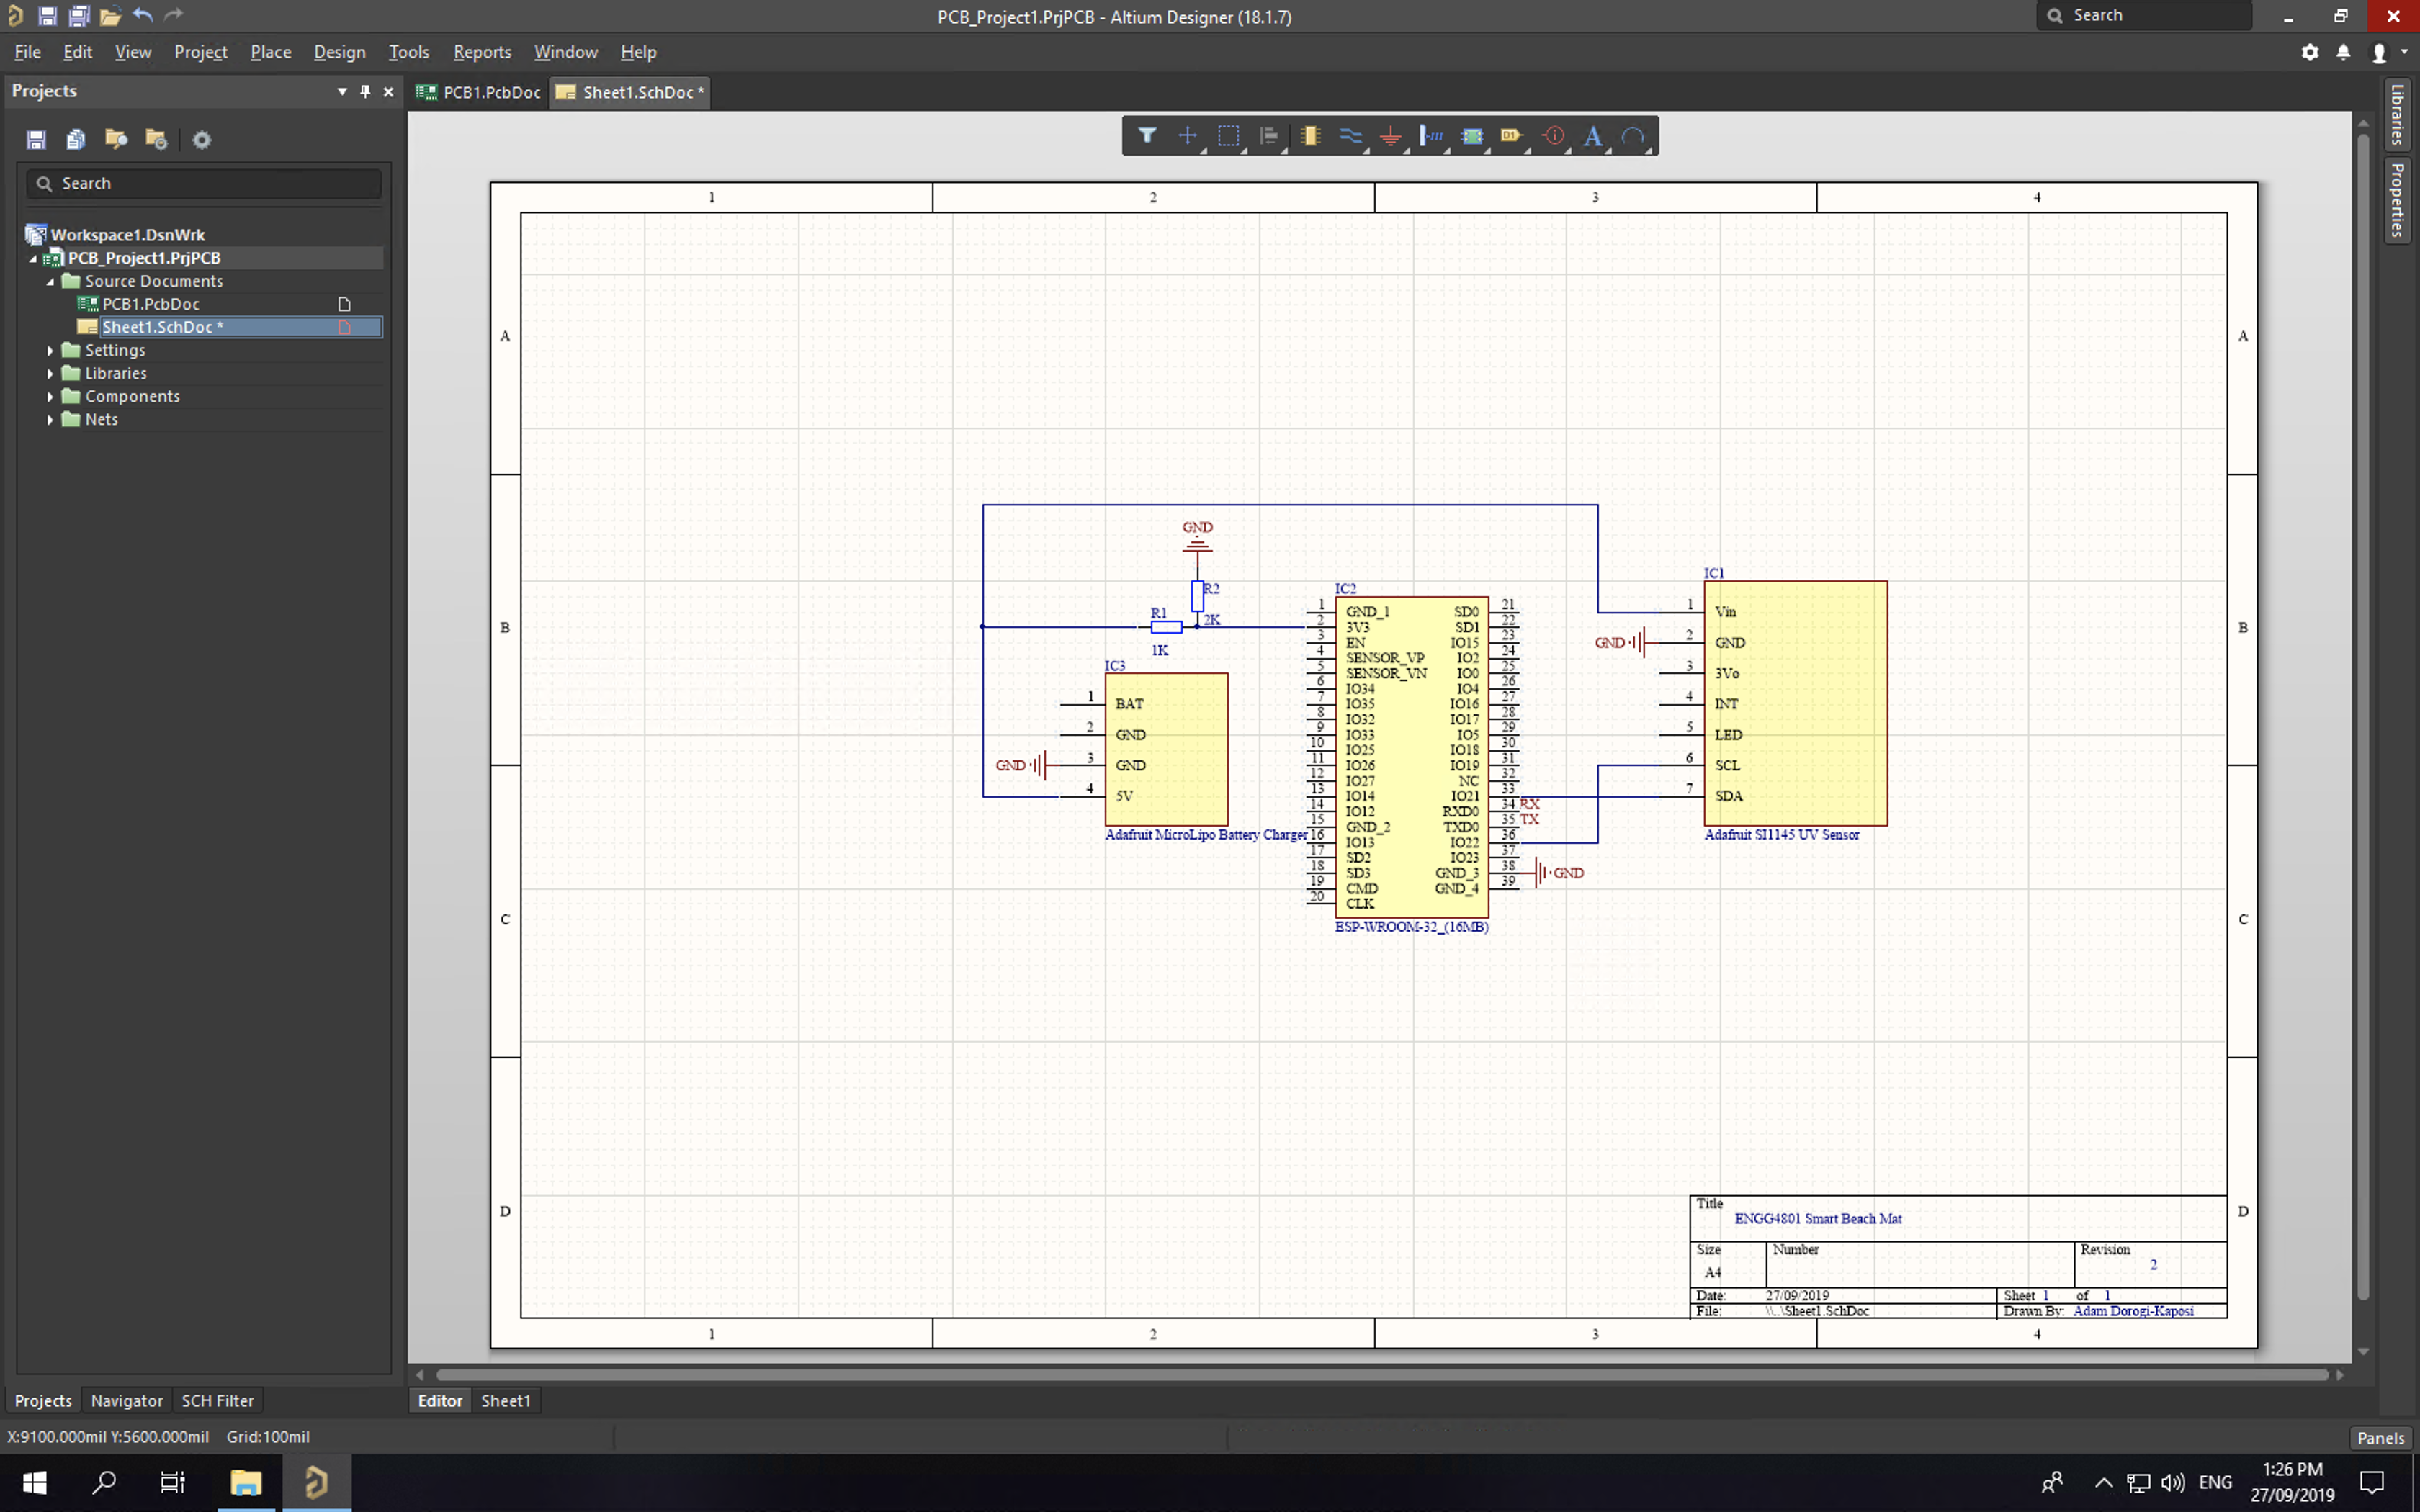
\includegraphics[width=\textwidth]{altium_final_schematic_2.png}
\caption{Schematic of final PCB during development in Altium Studio}
\label{fig:schematic_screenshot}
\end{figure}

\begin{figure}[h]
\centering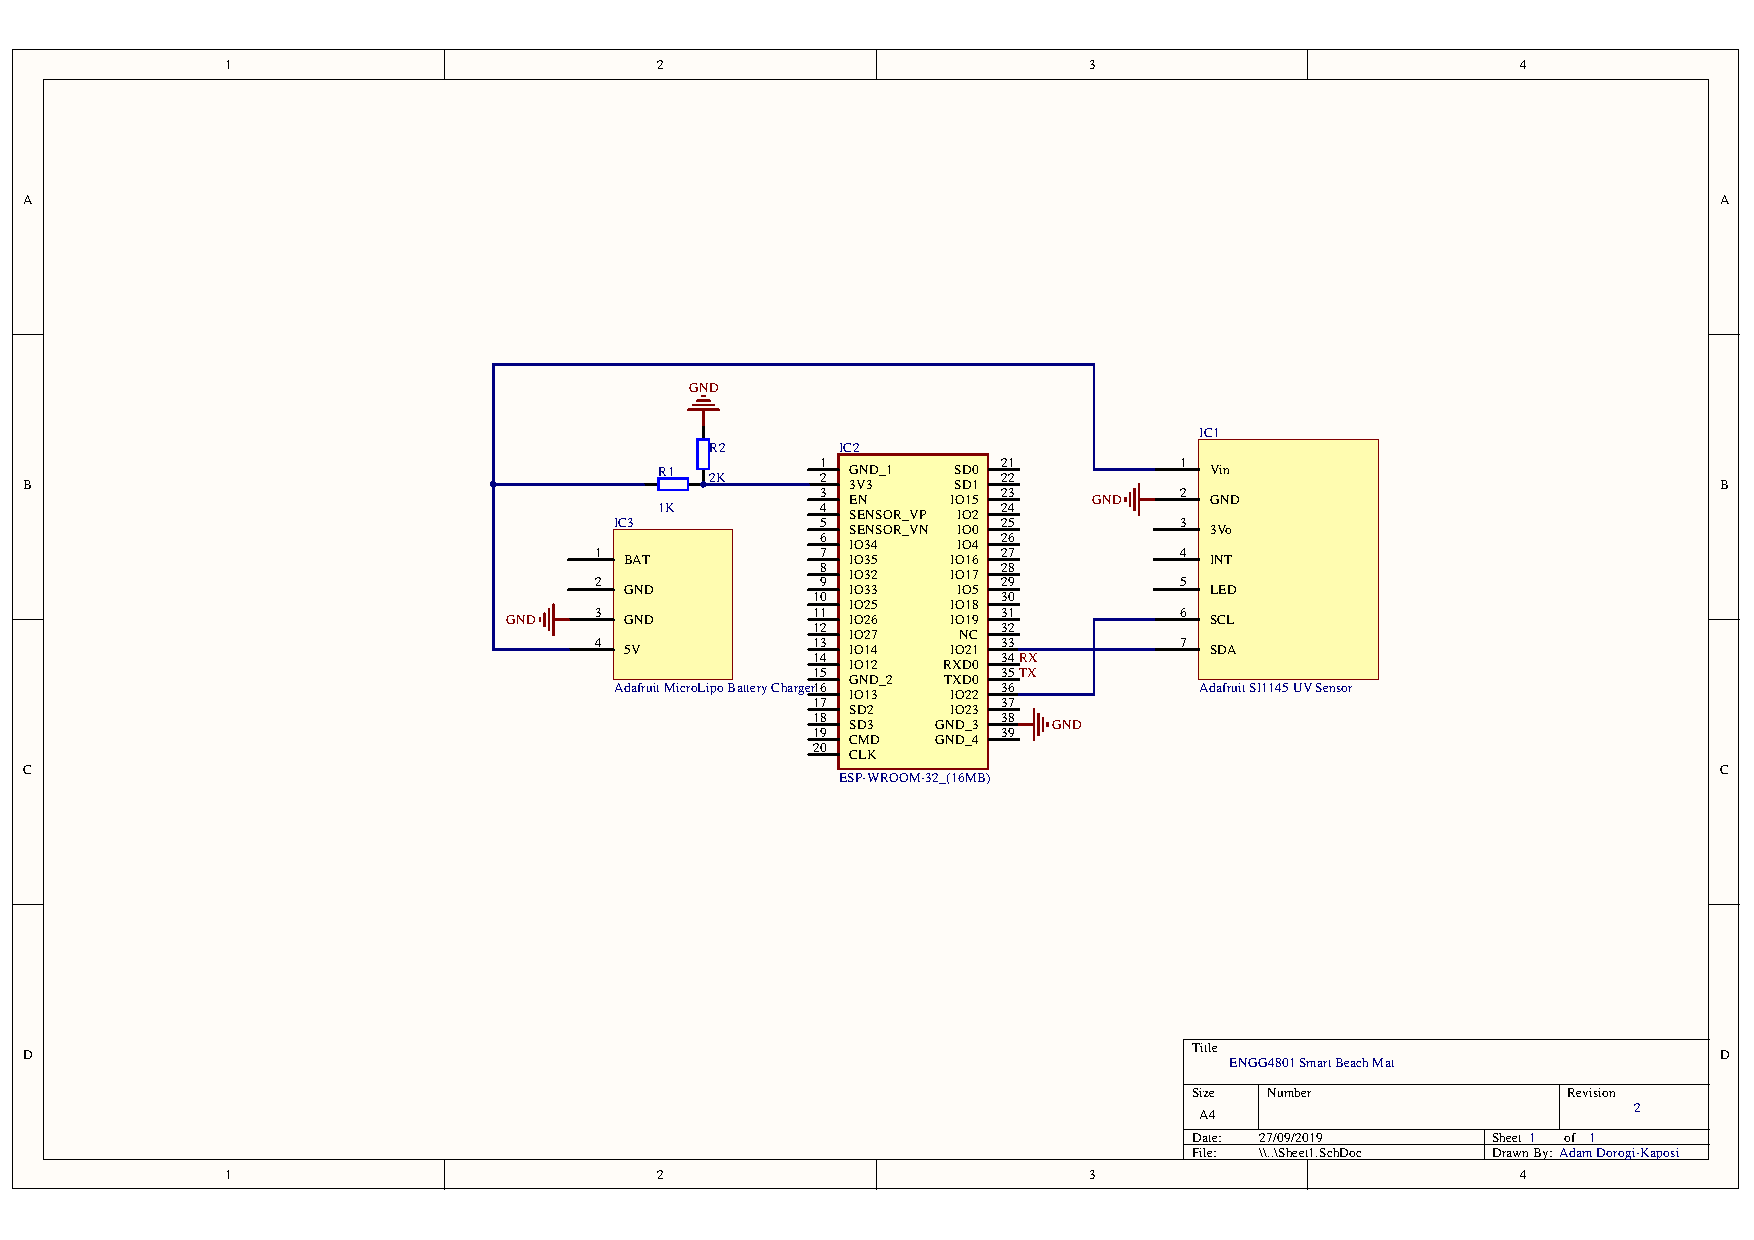
\includegraphics[width=\textwidth]{altium_final_pdf_2.pdf}
\caption{Schematic of final PCB}
\label{fig:schematic_pdf}
\end{figure}

It can be seen
that two resistors have been added to the circuit, to drop the voltage from 5\V\
to apprixmately 3.3\V, which is what the ESP32 and the SI1145 UV sensor needs to run on. The values of the
resistors are 1\kohm\ and 2\kohm. To get these values, \eq{eq:voltage_drop} was used.

\begin{equation}
\label{eq:voltage_drop}
V_{out} = V_{in} \cdot \frac{R_2}{R_1 + R_2}
\end{equation}

Since we wanted an output voltage of around 3.3\V, and the input voltage was 5\V,
$R_1$ and $R_2$ values of 1\kohm\ and 2\kohm\ were needed to satisfy the equation.

The size of the battery was determined by checking the current draw of the
prototype shown in \fig{fig:prototype}, by connecting it to a power supply.
This setup can be seen in \fig{fig:current_draw}.

\begin{figure}[h]
\centering\includegraphics[width=\textwidth]{CurrentDraw.jpg}
\caption{Current draw of prototype}
\label{fig:current_draw}
\end{figure}

The circuit of the prototype drew in the range
of 70\mA to 100\mA. Thus it was decided that a 3.7\V battery to be used, size
2000 mAh. This will provide a battery life of roughly 28 hours, which can be
calculated by dividing the Ampere hours by the current draw of the device ($2000/70$).

This is battery is also convenient, since the size of the battery closely
resembles the size of the PCB, so it will be able to fit underneath without
occupying extra space.

The Alatium  components for the three components; the UV sensor, the USB battery
charger, and the ESP32 can be seen in \fig{fig:altium_uv_sensor}, \fig{fig:altium_usb_charger}, and \fig{fig:altium_esp32} respectively.

\begin{figure}[h]
\centering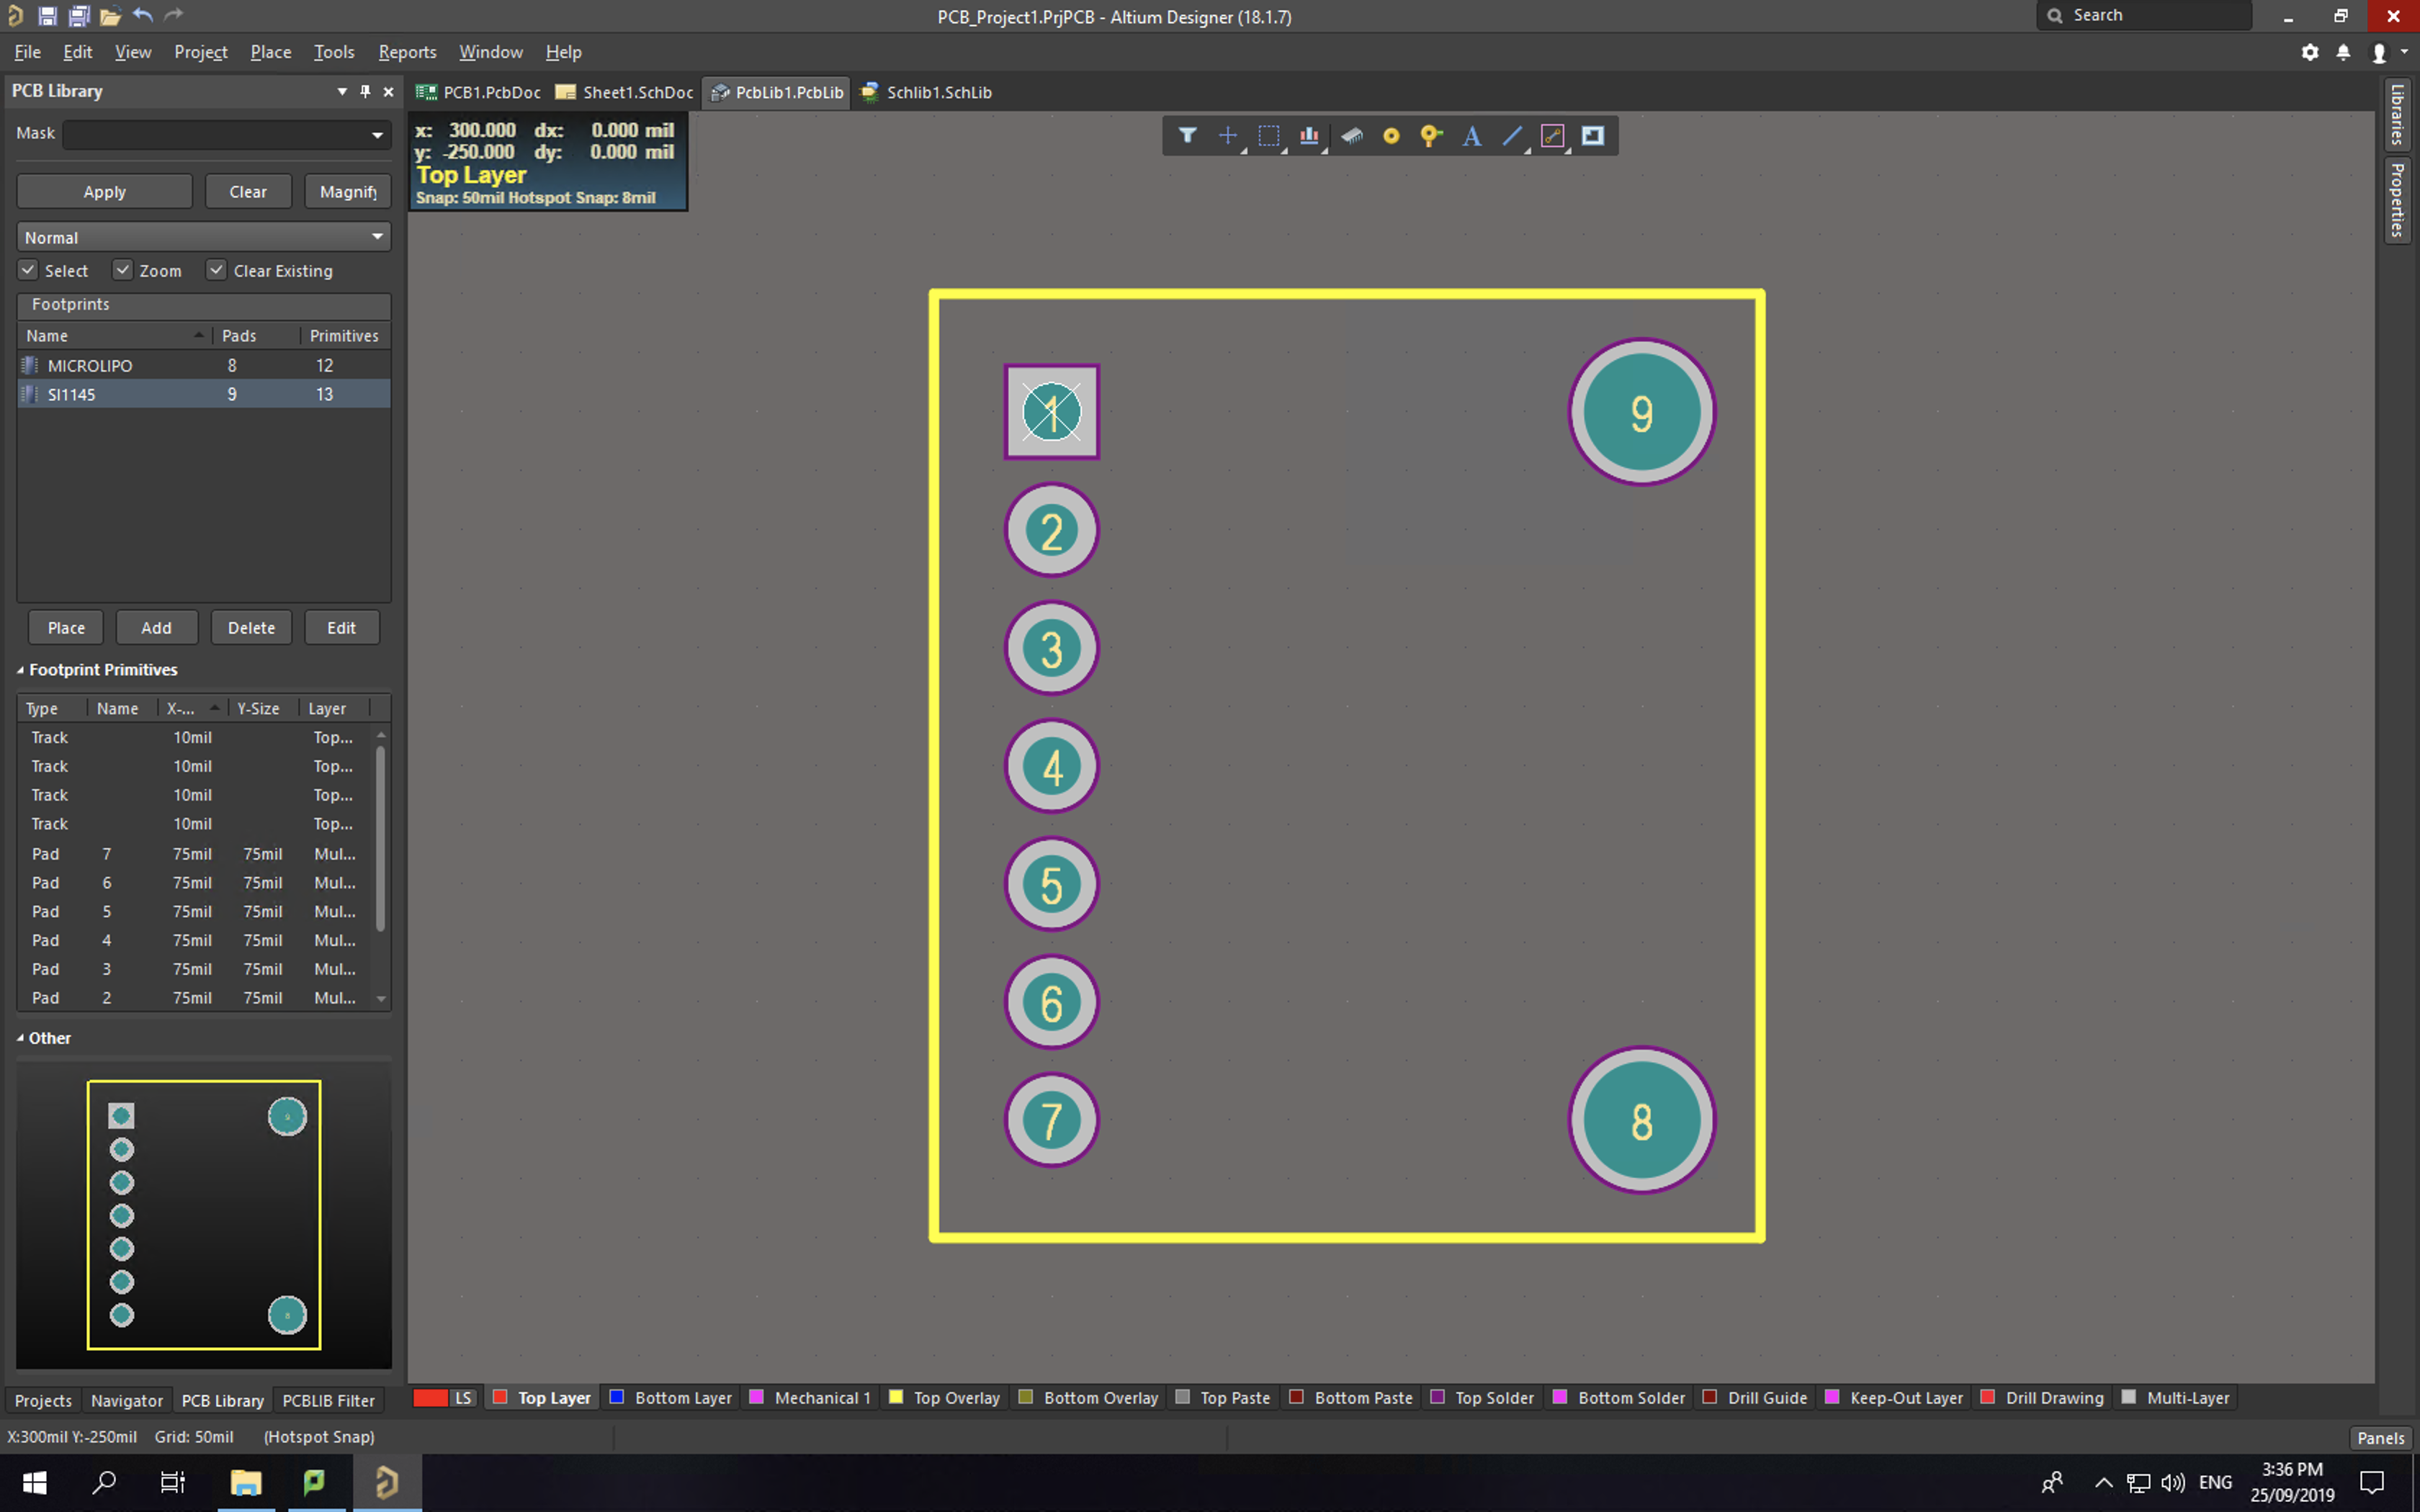
\includegraphics[width=\textwidth]{altium_uv_sensor.png}
\caption{PCB print of SI1145 UV Sensor}
\label{fig:altium_uv_sensor}
\end{figure}

\begin{figure}[h]
\centering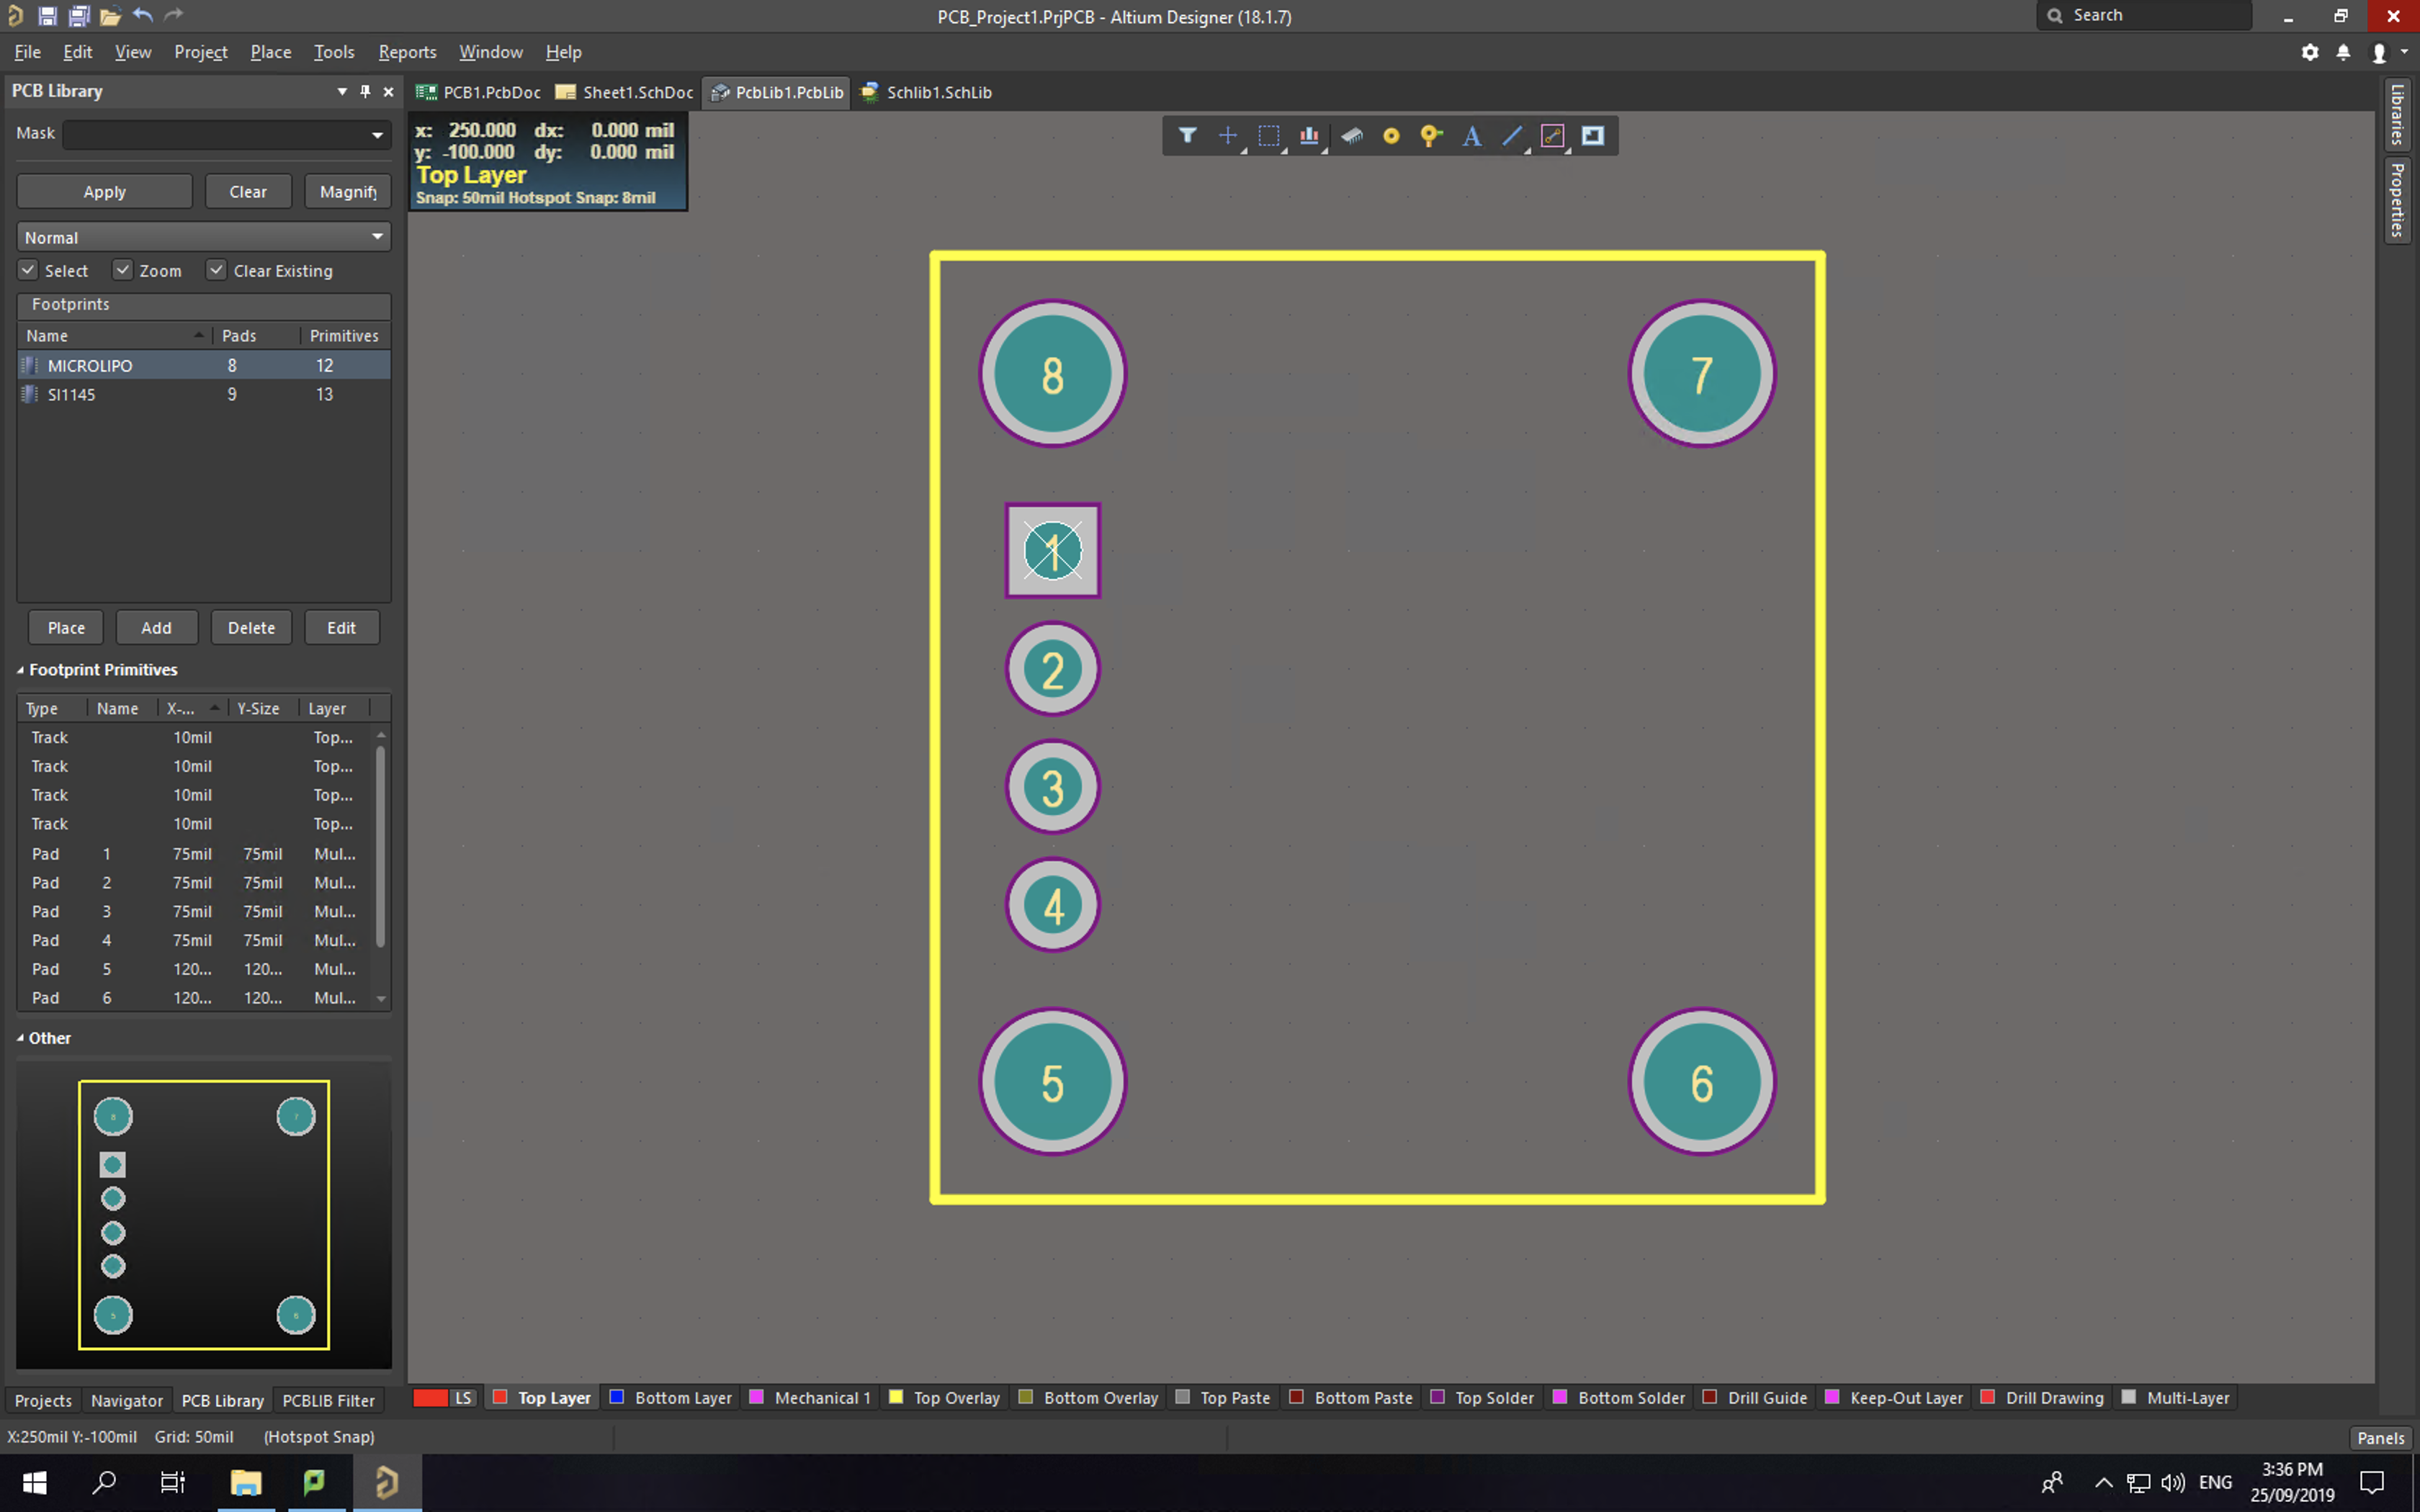
\includegraphics[width=\textwidth]{altium_usb_charger.png}
\caption{PCB Print of USB charger}
\label{fig:altium_usb_charger}
\end{figure}

\begin{figure}[h]
\centering\includegraphics[width=\textwidth]{altium_esp32.png}
\caption{PCB Print of ESP32}
\label{fig:altium_esp32}
\end{figure}

The Altium model components combined onto a single PCB can be seen in \fig{fig:altium_final}.


\begin{figure}[h]
\centering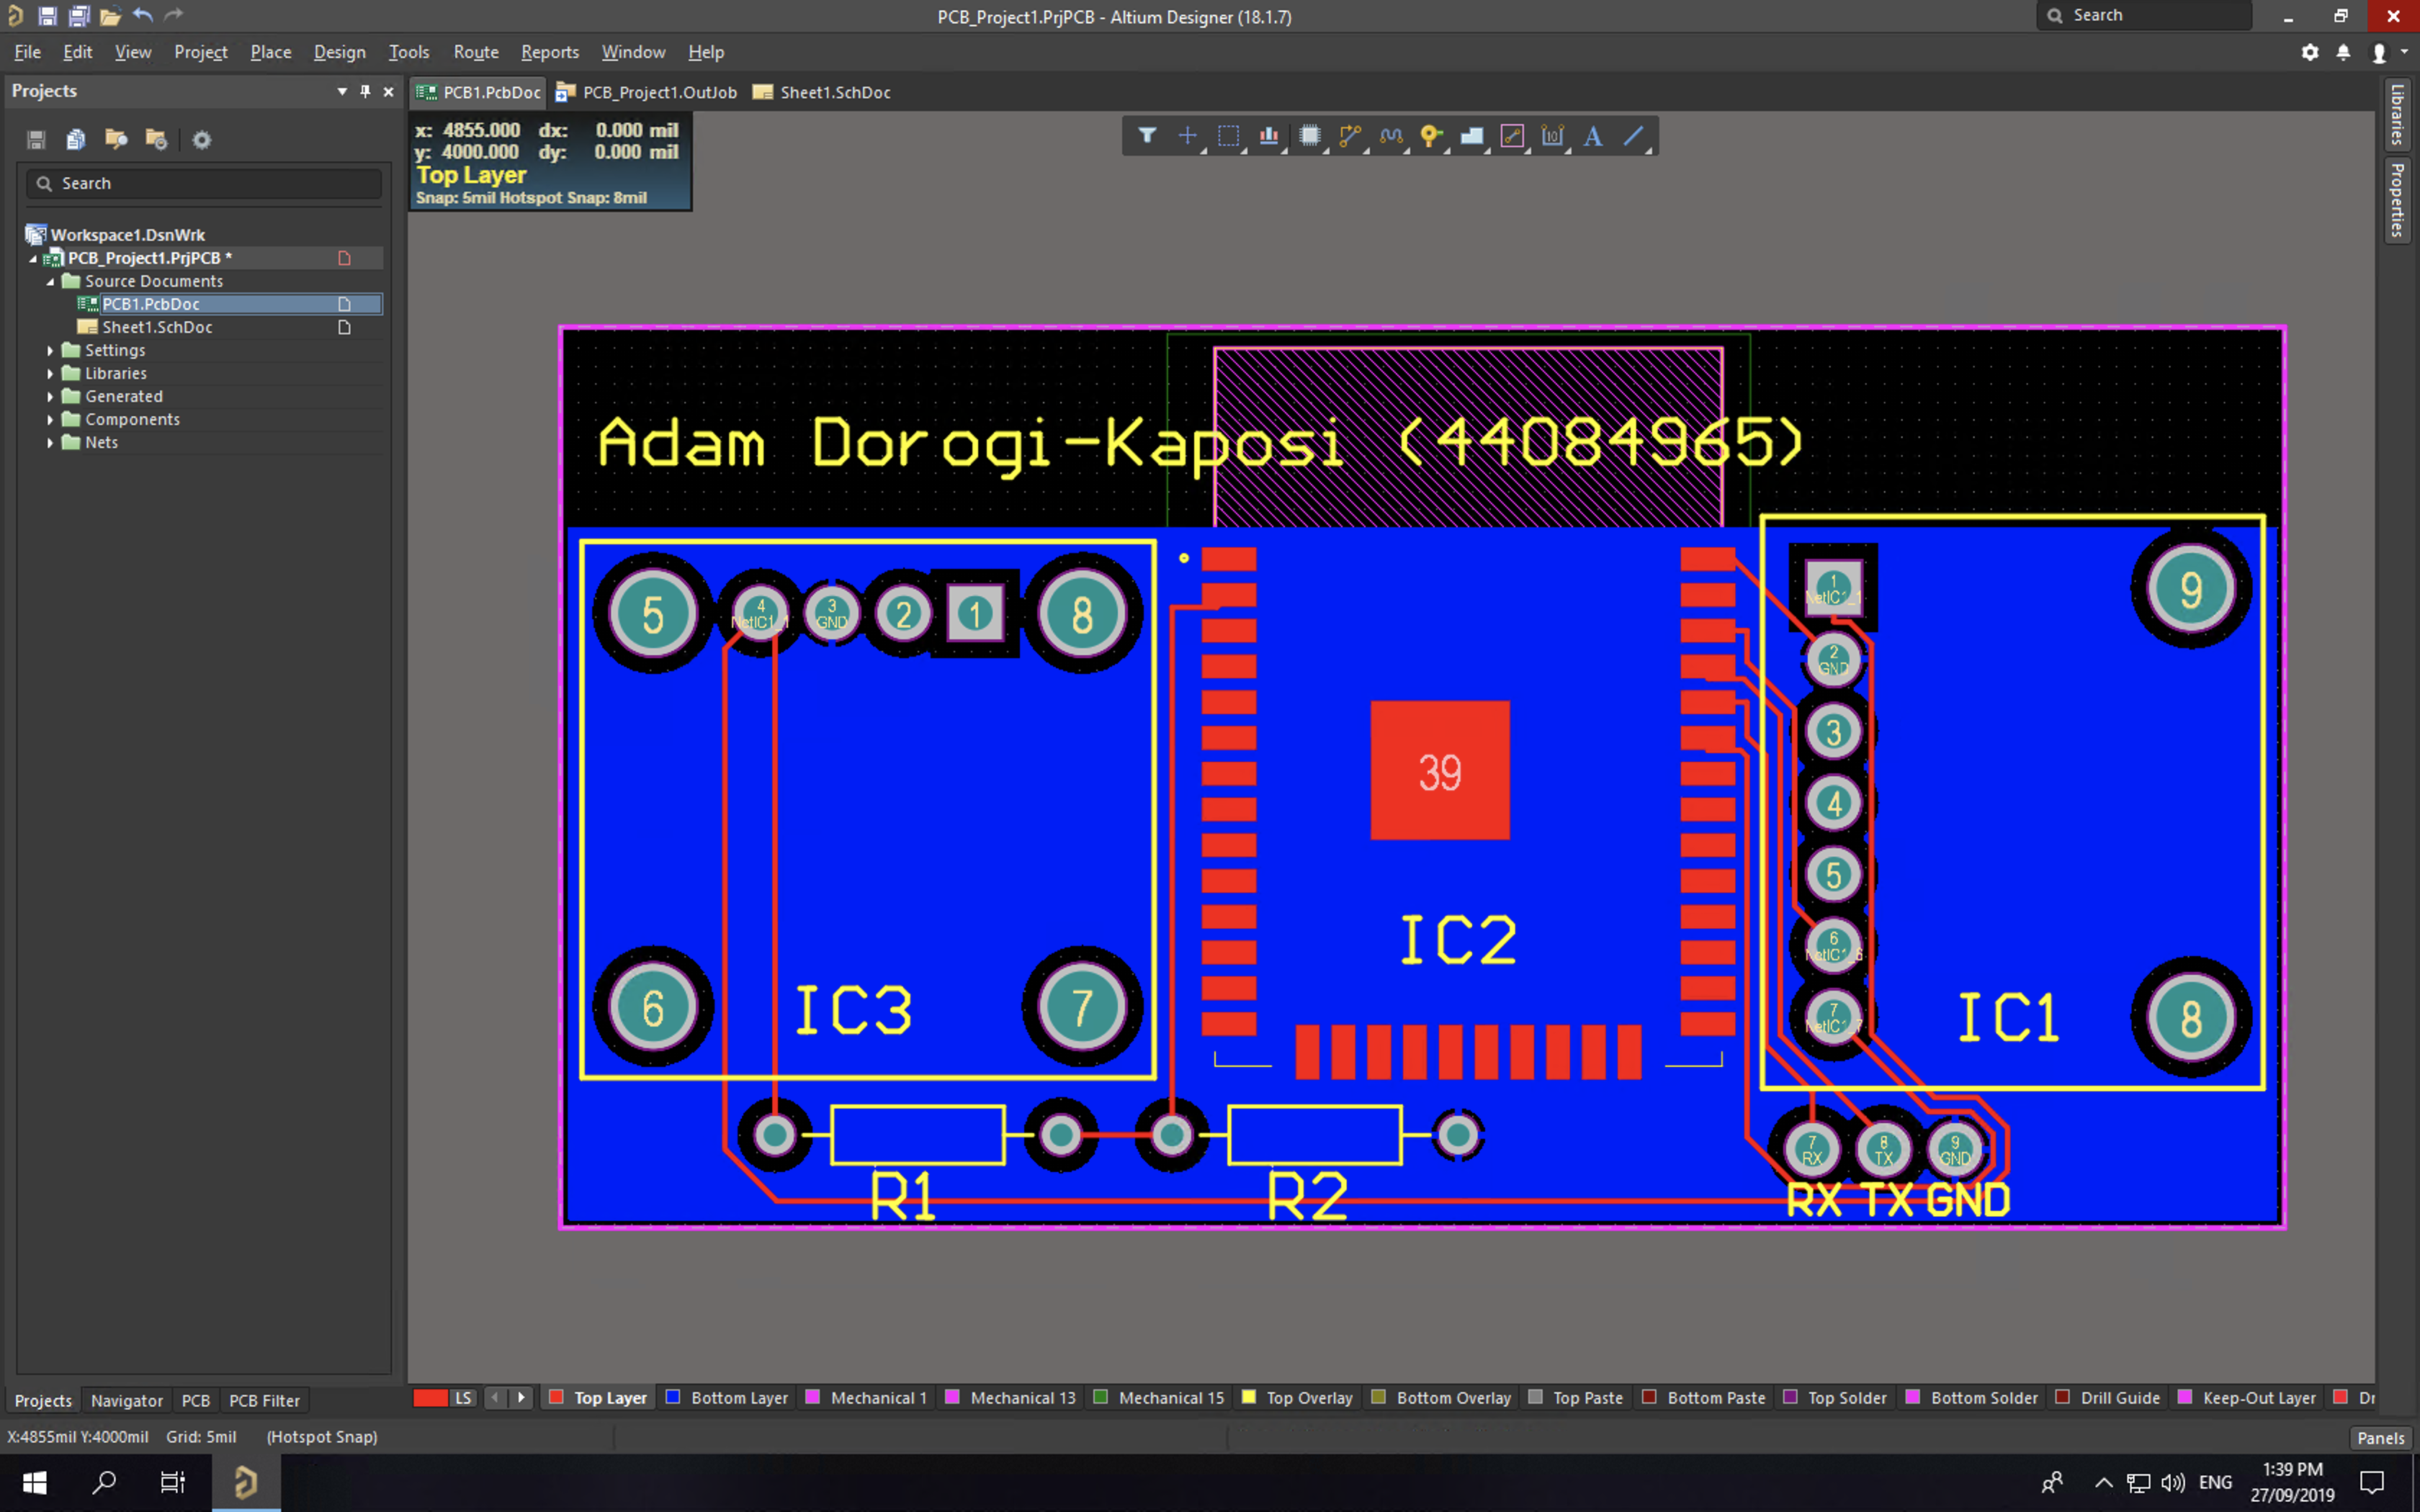
\includegraphics[width=\textwidth]{altium_final.png}
\caption{Final PCB design}
\label{fig:altium_final}
\end{figure}

%TODO
% The final PCB was printed, and can be seen in \fig{}.
% Casing

\section{Database}

\subsection{Schema}

The database was named \verb|smart_beachmat_database|. The schema for the database for storing user related information consists of
4 entities; account, user, reading, token. A detailed explanation of each entity
can be found in \secn{secn:tables}. The ER diagram for the schema can be seen in \fig{fig:er}.

\begin{figure}[h]
	\centering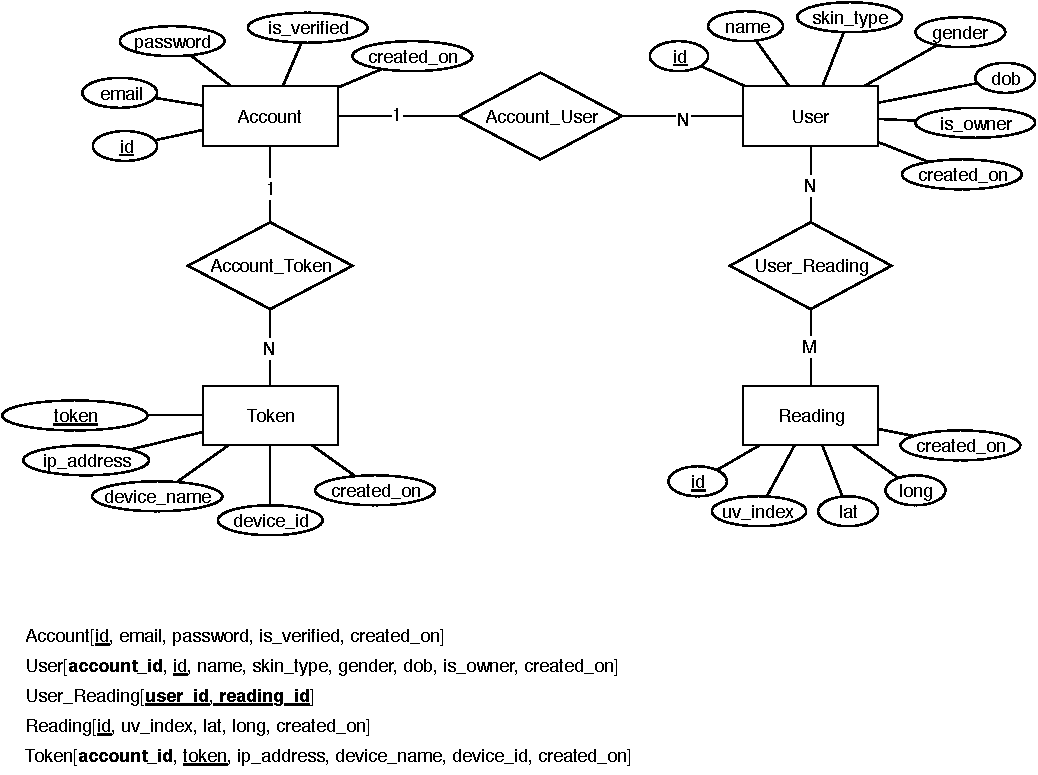
\includegraphics[width=\textwidth]{er.pdf}
	\caption{ER Diagram of Database Schema}
	\label{fig:er}
	\end{figure}

This corresponds to five tables; \verb|user|, \verb|account|, \verb|token|, \verb|reading|, \verb|user_reading|.

\subsection{Management}

Managed through phpmyadmin interface, with the root user. This user had all
privileges including deletion of tables and database. Used for creating tables,
setting up schema, and administrative purposes. However, an additional user was
created, with restricted privileges, was also created. This user is to access 
the database through the REST API, as discussed in \secn{secn:rest_api}. Due to security
considerations, privileges have been restricted for this user.

\subsection{Tables}
\label{secn:tables}

\subsubsection{Account}

The account entity represents an account created by the user, after registering
to the application.

The structure of the account table is:

\begin{itemize}
	\item \verb|id: binary(16)|
	\begin{itemize}
		\item The ID of the entity (randomly generated UUID)
	\end{itemize}
	\item \verb|email: varchar(254)|
	\begin{itemize}
		\item The email address of the account (must be in the correct format),
		varchar(254) because thats the longest an email can be [https://stackoverflow.com/questions/386294/what-is-the-maximum-length-of-a-valid-email-address].
	\end{itemize}
	\item \verb|password: varchar(255)|
	\begin{itemize}
		\item Hashed password of the account (using bcrytp). Varchar(255) as
		recommended by PHP [https://www.php.net/manual/en/function.password-hash.php].
	\end{itemize}
	\item \verb|is_verified: tinyint(1)|
	\begin{itemize}
		\item Boolean value indicating whether the email address of the account
		is verified. Default value 0 (false).
	\end{itemize}
	\item \verb|created_on: datetime|
	\begin{itemize}
		\item The date the account was created on. Default value
		CURRENT\_TIMESTAMP.
	\end{itemize}
\end{itemize}

\subsubsection{User}

The user represents a profile within an account. An account can have multiple
users, and only one owner user, responsible for the account.

The structure of the user table is:

\begin{itemize}
	\item \verb|id: binary(16)|
	\begin{itemize}
		\item The ID of the entity (randomly generated UUID) (not null)
	\end{itemize}
	\item \verb|account_id: binary(16)|
	\begin{itemize}
		\item The foreign key to the account ID that this user belongs to (not null).
	\end{itemize}
	\item \verb|name: varchar(64)|
	\begin{itemize}
		\item The name of the user (not null).
	\end{itemize}
	\item \verb|skin_type: tinyint(1)|
	\begin{itemize}
		\item The skin type of the user, stored as an integer (1-6), corresponding
		to the fitzpatrick scale (can be null).
	\end{itemize}
	\item \verb|gender: enum('m', 'f')|
	\begin{itemize}
		\item Gender of the user (can be null).
	\end{itemize}
	\item \verb|dob: date|
	\begin{itemize}
		\item Date of birth of the user (can be null).
	\end{itemize}
	\item \verb|is_owner: tinyint(1)|
	\begin{itemize}
		\item Boolean value as to whether the user is the owner of the account.
		Default value is 0 (false).
	\end{itemize}
	\item \verb|created_on: datetime|
	\begin{itemize}
		\item The date the account was created on. Default value
		CURRENT\_TIMESTAMP.
	\end{itemize}
\end{itemize}

\subsubsection{Reading}

A reading represents a UV Index reading. Multiple users can posess the same UV
reading (under the same account), and a user can have multiple UV readings.

The structure of the reading table is:

\begin{itemize}
	\item \verb|id: binary(16)|
	\begin{itemize}
		\item The ID of the entity (randomly generated UUID) (not null).
	\end{itemize}
	\item \verb|uv_index: tinyint(2)|
	\begin{itemize}
		\item The UV Index of the reading, stored as an integer (0-11) (not null).
	\end{itemize}
	\item \verb|lat: decimal(10,8)|
	\begin{itemize}
		\item Latitude of the reading, stored as a decimal (can be null).
	\end{itemize}
	\item \verb|lng: decimal(11,8)|
	\begin{itemize}
		\item Longitude of the reading, stored as a decimal (can be null).
	\end{itemize}
	\item \verb|created_on: datetime|
	\begin{itemize}
		\item The date the account was created on. Default value
		CURRENT\_TIMESTAMP.
	\end{itemize}
\end{itemize}

\subsubsection{User Reading}

A joining table between user and reading entities. This is used to establish
the many-to-many relationship between reading and user.

\begin{itemize}
	\item \verb|user_id: binary(16)|
	\begin{itemize}
		\item The foreign key to the user ID (not null).
	\end{itemize}
	\item \verb|reading_id: tinyint(2)|
	\begin{itemize}
		\item The foreign key to the reading ID (not null).
	\end{itemize}
\end{itemize}

\subsubsection{Token}

Token is used as a security measure, and is created upon logging in, and deleted
after logging out. Token is sent with most API requests, to authorize the client.

\begin{itemize}
	\item \verb|token: varchar(255)|
	\begin{itemize}
		\item The value of the token.
	\end{itemize}
	\item \verb|account_id: binary(16)|
	\begin{itemize}
		\item The foreign key to the account ID that this token belongs to (not null).
	\end{itemize}
	\item \verb|ip_address: int(4)|
	\begin{itemize}
		\item The IP address of the token (where it was created) stored as a
		4 byte integer (not null).
	\end{itemize}
	\item \verb|device_id: varchar(36)|
	\begin{itemize}
		\item The ID of the device where the token was created (not null).
	\end{itemize}
	\item \verb|device_name: varchar(255)|
	\begin{itemize}
		\item The name of the device where the token was created (not null).
	\end{itemize}
	\item \verb|created_on: datetime|
	\begin{itemize}
		\item The date the account was created on. Default value
		CURRENT\_TIMESTAMP.
	\end{itemize}
\end{itemize}

\section{REST API}
\label{secn:rest_api}

The REST API was designed in order to interact with the 4 main entities
discussed in \secn{secn:tables}. The API endpoints for certain CRUD operations 
are seen below.

\subsection{Account}

\begin{table}[h]
\caption{\sl API endpoints for account entity.}
\label{tab:endpoint_account}
\begin{center}
\begin{tabularx}{\linewidth}{|l|X|X|X|X|}
\hline
Resource & \verb|POST| & \verb|GET| & \verb|PUT| & \verb|DELETE| \\
\hline
\verb|/v1/accounts| & Create account. & Get account information. & -- & Delete account. \\
\verb|/v1/accounts/email| & -- & -- & Update account email. & -- \\
\verb|/v1/accounts/password| & -- & -- & Update account password. & -- \\
\hline
\end{tabularx}
\end{center}
\end{table}

\subsubsection{Create an Account}

Endpoint: \verb|POST /v1/accounts|

Request Body:

\begin{verbatim}
email: must be a valid email format
password: must be at least 8 chars long (checked client side for confirmation)
\end{verbatim}

Required Headers:

\begin{verbatim}
none
\end{verbatim}

Response: 201 code on successful account creation.

\subsubsection{Get an Account's Information}

Endpoint: \verb|GET /v1/accounts|

Body:
\begin{verbatim}
none
\end{verbatim}

Required Headers: 

\begin{verbatim}
Authorization = Bearer XXX : a valid token belonging to the account
\end{verbatim}

Response: 200 code on successful get, plus:

\begin{verbatim}
{
	"id": "83e39d48-fde2-11e9-86a2-8d250fdf3259",
	"email": "adam2@gmail.comalk",
	"is_verified": false,
	"created_on": "2019-11-03 12:34:52"
}
\end{verbatim}

\subsubsection{Update Account Email}

Endpoint: \verb|PUT /v1/accounts/email|

Body:
new\_email: new email address, must be correct format
password: current password

\begin{verbatim}
new_email: new email address, must be correct format
password: current password
	\end{verbatim}

Required Headers: 

\begin{verbatim}
Authorization = Bearer XXX : a valid token belonging to the account
\end{verbatim}

Response: 204 code on successful update.

\subsubsection{Update Account Password}

Endpoint: \verb|PUT /v1/accounts/password|

Body:

\begin{verbatim}
password: current password
new_password: new password, must be at least 8 chars.
\end{verbatim}

Required Headers: 

\begin{verbatim}
Authorization = Bearer XXX : a valid token belonging to the account
\end{verbatim}

Response: 204 code on successful update.

\subsubsection{Delete an Account}

Endpoint: \verb|DELETE /v1/accounts|

Body:

\begin{verbatim}
none
\end{verbatim}

Required Headers: 

\begin{verbatim}
Authorization = Bearer XXX : a valid token belonging to the account
\end{verbatim}

Response: 204 code on successful delete.

\subsection{User}

\begin{table}[h]
\caption{\sl API endpoints for user entity.}
\label{tab:endpoint_user}
\begin{center}
\begin{tabularx}{\linewidth}{|l|X|X|X|X|}
\hline
Resource & \verb|POST| & \verb|GET| & \verb|PUT| & \verb|DELETE| \\
\hline
\verb|/v1/users| & Create user for account. & Get all users for account. & -- & -- \\
\verb|/v1/users/:id| & -- & -- & Update user with given ID. & Delete user with given ID. \\
\hline
\end{tabularx}
\end{center}
\end{table}

\subsubsection{Create a User}

Endpint: \verb|POST /v1/users|

Body:
\begin{verbatim}
name
skin_type: 1-6 (optional)
dob: yyyy-mm-dd (optional)
gender: m or f (optional)
\end{verbatim}

Required Headers: 

\begin{verbatim}
Authorization = Bearer XXX : a valid token belonging to the account
\end{verbatim}

Response: 201 code on successful creation.

\subsubsection{Get a User's Information}

\verb|GET /v1/users|

Body:

\begin{verbatim}
none
\end{verbatim}

Required Headers: 

\begin{verbatim}
Authorization = Bearer XXX : a valid token belonging to the account
\end{verbatim}

Response: 200 code on successful get, plus:

\begin{verbatim}
{
	"id"
	"name"
	"skin_type"
	"gender"
	"dob"
	"is_owner"
	"created_on"
}
\end{verbatim}

\subsubsection{Update a User}

Endpoint: \verb|PUT /v1/users/:id|

Body:
\begin{verbatim}
name:
skin_type: 1-6 (optional)
dob: yyyy-mm-dd (optional)
gender: m or f (optional)
\end{verbatim}

Required Headers: 

\begin{verbatim}
Authorization = Bearer XXX : a valid token belonging to the account
\end{verbatim}

Response: 204 code on successful update.

\subsubsection{Delete a User}

Endpoint: \verb|DELETE /v1/users/:id|

Body:
\begin{verbatim}
none
\end{verbatim}

Required Headers: 

\begin{verbatim}
Authorization = Bearer XXX : a valid token belonging to the account
\end{verbatim}

Response: 204 code on successful delete.

\subsection{Token}

\begin{table}[h]
\caption{\sl API endpoints for token entity.}
\label{tab:endpoint_token}
\begin{center}
\begin{tabularx}{\linewidth}{|l|X|X|X|X|}
\hline
Resource & \verb|POST| & \verb|GET| & \verb|PUT| & \verb|DELETE| \\
\hline
\verb|/v1/tokens| & Create token for account. & Get all device IDs belonging to token. & -- & Delete token. \\
\hline
\end{tabularx}
\end{center}
\end{table}

\subsubsection{Create a Token (Login)}

Endpoint: \verb|POST /v1/tokens|

Body:

\begin{verbatim}
email: email to log in
password: password to log in
\end{verbatim}

Required Headers:

\begin{verbatim}
none
\end{verbatim}

Response: 201 code on successful creation, plus:

\begin{verbatim}
{
	"token":"7fd15938c823cf58e78019bea2af142f9449696a"
}
\end{verbatim}

\subsubsection{Get a Token}

Get all device IDs corresponding to tokens belonging to account (for given token).

Endpoint: \verb|GET /v1/tokens|

Body:
\begin{verbatim}
none
\end{verbatim}

Required Headers:

\begin{verbatim}
Authorization = Bearer XXX : a valid token belonging to the account
\end{verbatim}

Response: 200 code on successful get, plus:

\begin{verbatim}
[
	{
		"ip_address": "12.34.56.78",
		"device_id": "aaaa-aaaa-aaaa-aaaaaaaa",
		"device_name": "Adam's iPhone",
		"created_on": "2019-11-03 15:29:52"
	}
]
\end{verbatim}

\subsubsection{Delete a Token}

Endpoint: \verb|DELETE /v1/tokens|

Body:

\begin{verbatim}
device_id: id of device to revoke token
\end{verbatim}

Required Headers: 

\begin{verbatim}
Authorization = Bearer XXX : a valid token belonging to the account
\end{verbatim}

Response: 204 code on successful delete.

\subsection{Reading}

\begin{table}[h]
\caption{\sl API endpoints for reading entity.}
\label{tab:endpoint_reading}
\begin{center}
\begin{tabularx}{\linewidth}{|l|X|X|X|X|}
\hline
Resource & \verb|POST| & \verb|GET| & \verb|PUT| & \verb|DELETE| \\
\hline
\verb|/v1/readings| & Create token for account. & -- & -- & -- \\
\verb|/v1/readings/:id| & -- & Get all device IDs belonging to token. & -- & -- \\
\hline
\end{tabularx}
\end{center}
\end{table}

\subsubsection{Create a Reading}

Endpoint: \verb|POST /v1/readings|

Body:

\begin{verbatim}
user_ids: ids of users to post reading to (comma separated)
uv_index: the UV Index to post
lat: latitude of UV Index
lng: longitude of UV Index
\end{verbatim}

Required Headers: 

\begin{verbatim}
Authorization = Bearer XXX : a valid token belonging to the account
\end{verbatim}

Response: 201 code on successful creation.

\subsubsection{Get a Reading}

Endpoint: \verb|GET /v1/readings/:user_id|

Body:

\begin{verbatim}
none
\end{verbatim}

Required Headers: 

\begin{verbatim}
Authorization = Bearer XXX : a valid token belonging to the account
\end{verbatim}

Response: 200 code on successful get, plus:
\begin{verbatim}
[
	{
		"uv_index": "9",
		"lat": "80.00000000",
		"lng": "120.00000000",
		"created_on": "2019-11-03 15:39:36"
	}
]
\end{verbatim}

\subsection{Structure}
\label{secn:structure}

The file structure for the API workspace was as follows.

\dirtree{%
.1 smart\_beachmat\_server.
.2 phpMyAdmin.
.3 \dots.
.2 README.md.
.2 v1.
.3 classes.
.4 Account.php.
.4 Reading.php.
.4 Token.php.
.4 User.php.
.3 config.
.4 config.php.
.4 Database.php.
.3 index.php.
}

As seen previously, the Apache configuration file had to be modified in order to
point to this directory; i.e. when the server started, it would look for an index file in this directory.

However, in order to conform to both the API endpoints specified in
\tab{tab:endpoint_account}\dots\tab{tab:endpoint_reading} with the given directory
structure, URL rewriting had to be
enabled on the server, to redirect all requests, regardless of the resource, to
the index.php file. Once the request has been redirected to index.php, we can
determine where to go from there, based on what the user initially requested.

To enable the URL rewriting, the apache config file had to be modified, and the
following line had to be uncommented.

\begin{verbatim}
#LoadModule rewrite_module libexec/apache2/mod_rewrite.so
\end{verbatim}

%TODO
% The URL rewriting rules are specified in a .htaccess file, at the root of the
% server directory. By default however, the .htaccess file is disabled in the
% apache config file. To enable this, we had to change
% %see readme
% to this
% %see readme
% .

After doing so, rewrite rules could be specified to the server. To specify the
needed rewrite rules for this scenario, the following had been added to the
.htaccess file.

\begin{verbatim}
RewriteEngine On
RewriteRule ^v1/ v1/index.php
\end{verbatim}

This rule states that all traffic going to map the request going to any resource
starting with v1 to the v1/index.php file.

Since all traffic is routed to index.php, we have a central space to handle the
requests, and call corresponding logic accordingly, based on the given URL.

For example, if a request to /v1/accounts is made, the url will be mapped to
index.php. In the index.php file, we will see that /v1/accounts has been
requested. Based on this information, we create a new Account object. In the
Account object initiation, we do further processing of the request, such as
checking the HTTP request method, any body parameters, or whether the URL
has additional components, such as /v1/accounts/email. Based on these checks,
we manipulate or query the database accordingly.

%TODO
% The index.php file can be seen
% in \app{}, and the full REST API project can be seen in \app{}.

\section{Smartphone Application}

Developed using Flutter, the cross-platform smartphone application was designed
to interact with the REST API, and the IoT device.

\subsection{Design}

To begin the development process, a low-fidelity prototype was created, to
brainstorm and ideate the necessary screens to cover all REST API functions,
to make the flow between screens as smooth as possible, and to have a fixed set
of requirements while developing the application, as opposed to free balling.
The low fidelity prototype can be found in \fig{fig:low_fid}.

\begin{figure}[h]
\centering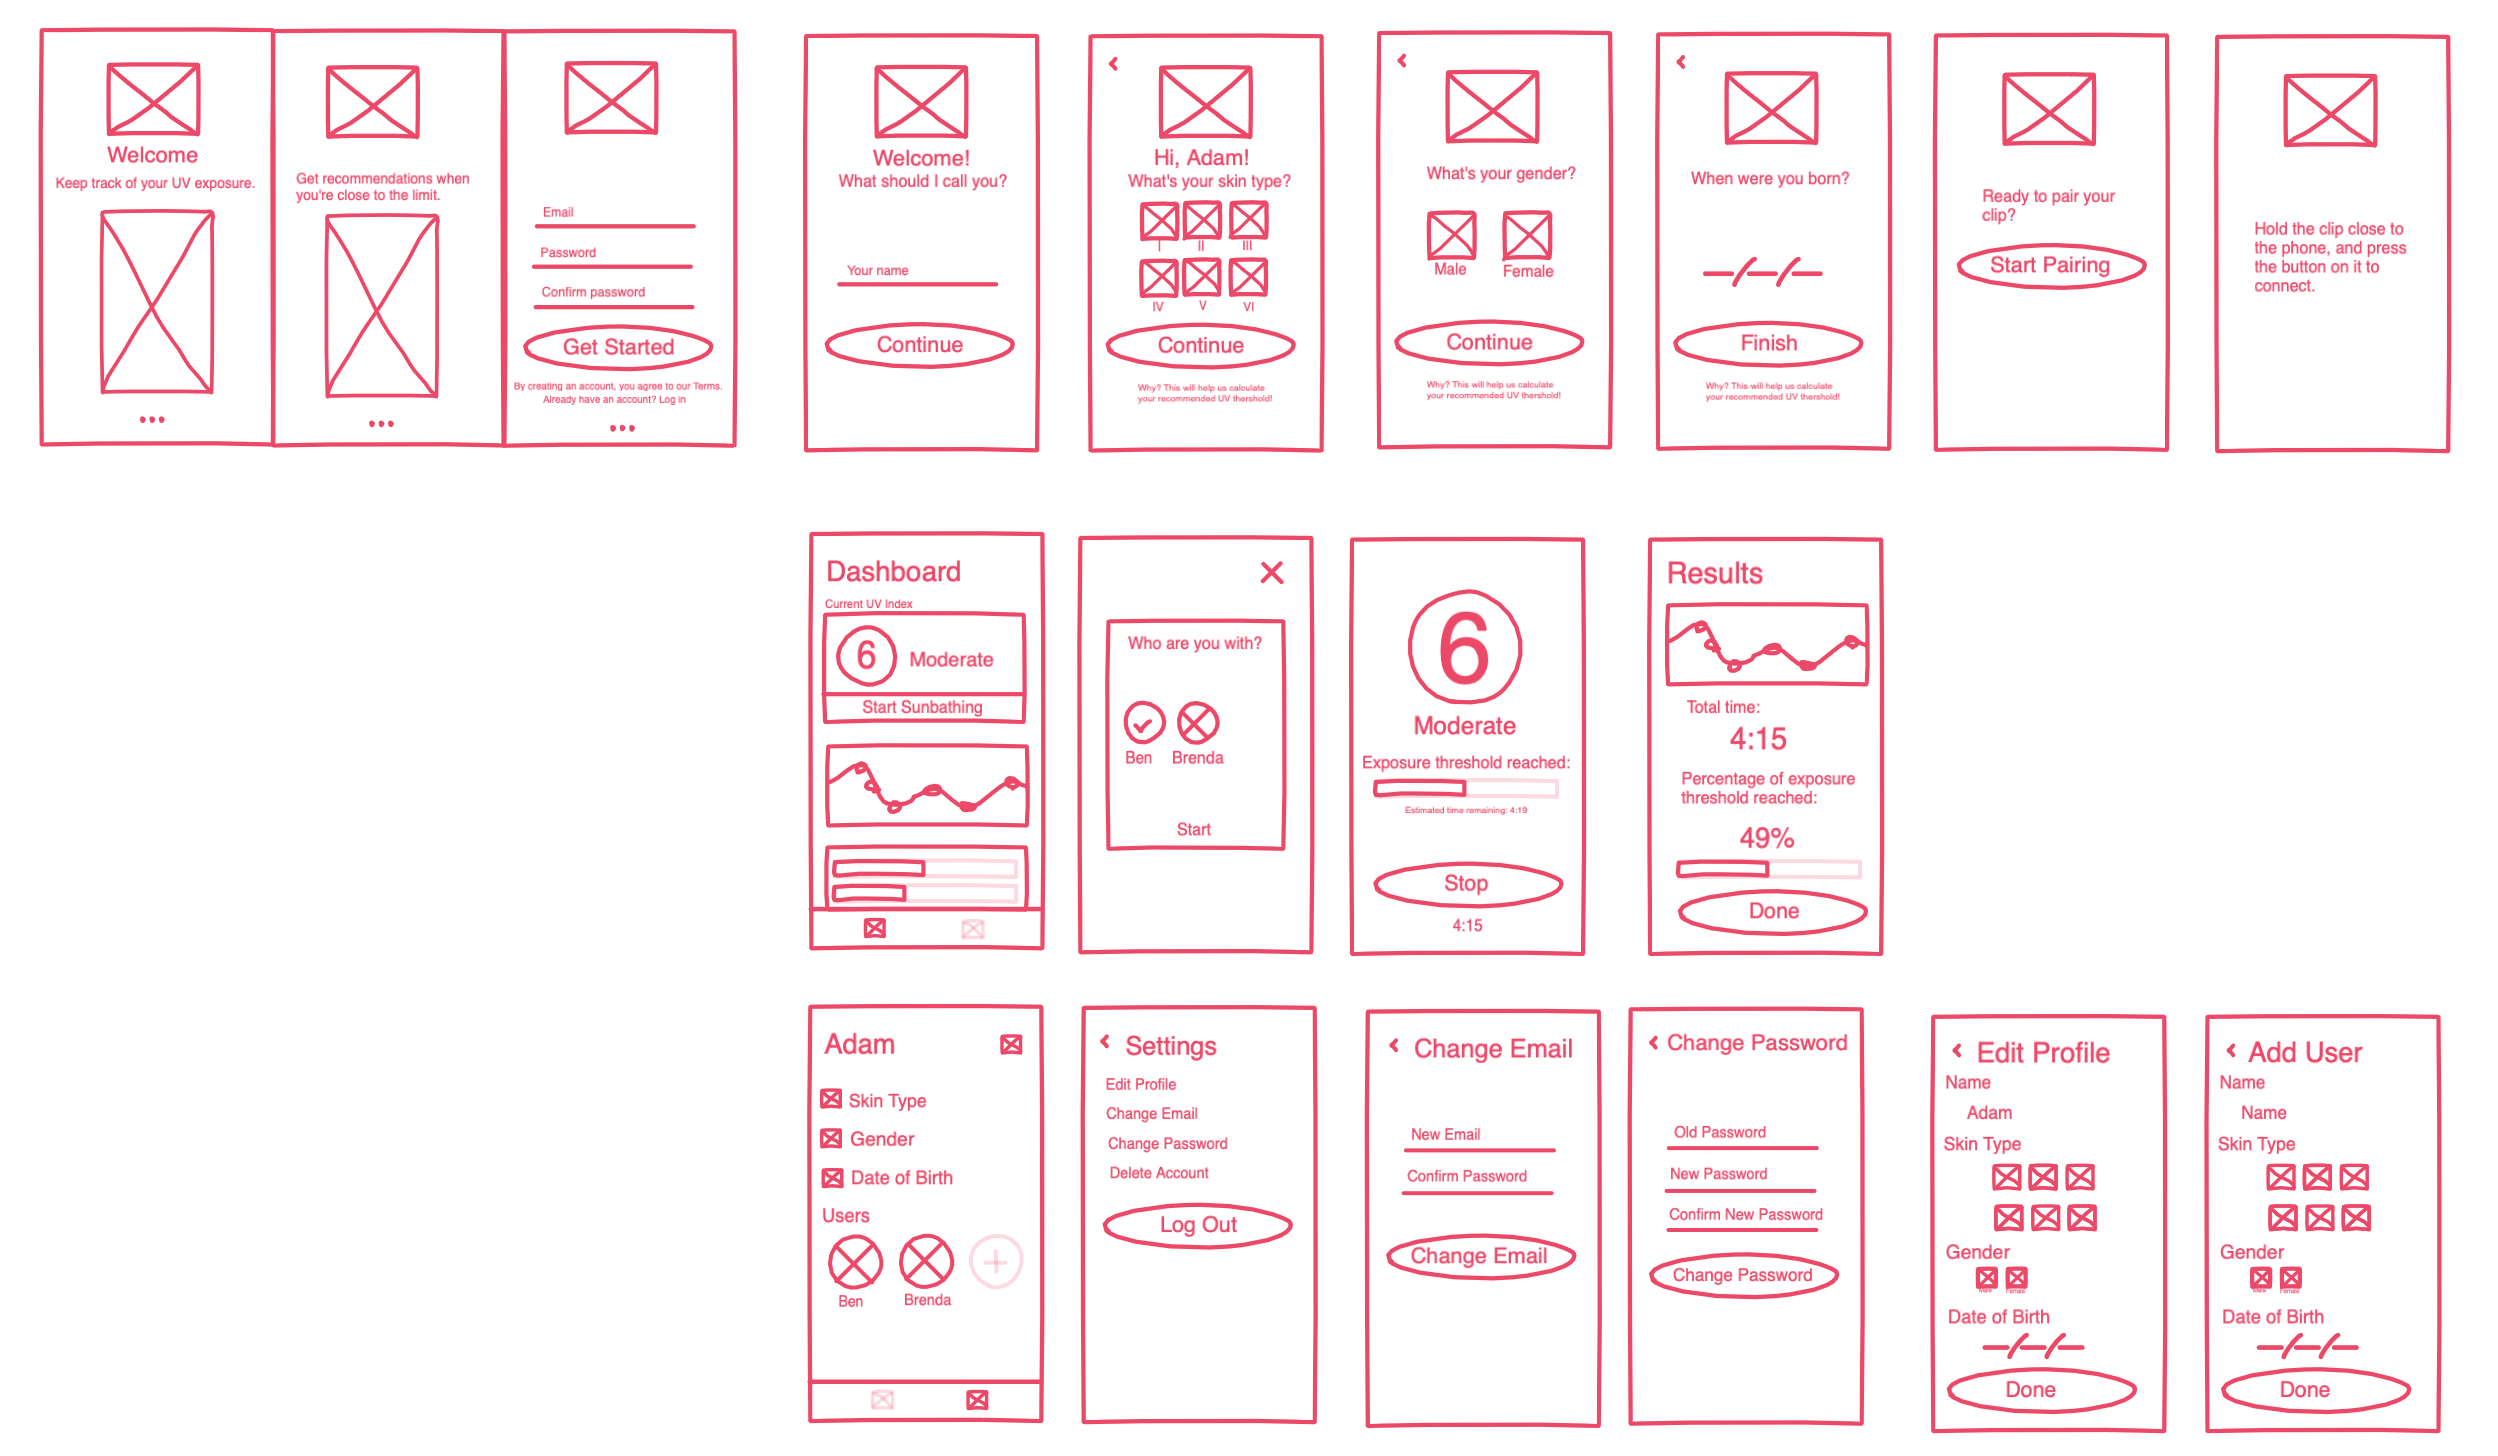
\includegraphics[width=\textwidth]{LowFid.png}
\caption{Low-fidelity prototype of smartphone application}
\label{fig:low_fid}
\end{figure}

\subsection{Final}

Secure storage was used to store tokens, as tokens are considered a sensitive
piece of information. Anyone with access to a token may perform any API request
on the owner's behalf, which is considered as a security threat. Therefore, this
token is stored in a secure storage, corresponding to iOS's keychain, and
Android's keystore. This is a hardware level encrypted storage.

Local SQLite database was also used to store user information. Storing user
information was useful when determining whether a user was created for the account.
As an example, if an account logs in, and no users are stored in the local database,
the application makes an API request to get all users of the account. The returned users
are then stored in the local database. If no users are returned, i.e. no users are
stored in the local database, the application screen is redirected to the create user page.
Ensuring that the account will not be able to use the application unless at least one
user is created.

\subsection{Project Structure}

The file structure for the Flutter application is as follows.

\dirtree{%
.1 smart\_beachmat\_app.
.2 lib.
.3 bottom\_navigation\_scaffold.dart.
.3 dashboard\_widget.dart.
.3 main.dart.
.3 models.
.4 api\_exception.dart.
.4 api\_service.dart.
.4 database\_provider.dart.
.4 secure\_storage\_provider.dart.
.4 theme.dart.
.4 user.dart.
.3 profile\_widget.dart.
.3 screens.
.4 device\_connection\_scaffold.dart.
.4 log\_in.
.5 log\_in\_form.dart.
.5 log\_in\_scaffold.dart.
.4 sign\_up.
.5 dob.
.6 sign\_up\_dob\_form.dart.
.6 sign\_up\_dob\_scaffold.dart.
.5 email.
.6 sign\_up\_email\_form.dart.
.6 sign\_up\_email\_scaffold.dart.
.5 gender.
.6 sign\_up\_gender\_form.dart.
.6 sign\_up\_gender\_scaffold.dart.
.5 name.
.6 sign\_up\_name\_form.dart.
.6 sign\_up\_name\_scaffold.dart.
.5 skin\_type.
.6 sign\_up\_skin\_type\_form.dart.
.6 sign\_up\_skin\_type\_scaffold.dart.
.3 widgets.
.4 bottom\_navigation\_widget.dart.
.4 chip\_wrap.dart.
.4 left\_app\_bar.dart.
.4 sign\_up\_button.dart.
}

\verb|models| contains models such as user, as well as other classes which provide
interaction with the API (\verb|api_service|), the secure storage
(\verb|secure_storage_provider|), the theme definition (\verb|theme|), or local database
(\verb|database_provider|)

The main file is the starting point of the application, and based on certain logic,
such as whether the user is already logged in (i.e. a token is stored), corresponding
screens will be shown. The \verb|dashboard_widget| shows a screen for the dashboard,
and the \verb|profile_widget| shows a screen for the profile. Screens contains further
screens, such as login screen, sign up screen, and device connection scaffold.


The widgets folder contains certain widgets which have been modified (i.e.
subclassed) to provide certain UI behaviour, such as aligning the text of the
application bar to the left, and changing its font styles and size in \verb|left_app_bar|.

These screens, along with the screens of the final application, can be seen in
\fig{}.


\begin{figure}[h]
	\centering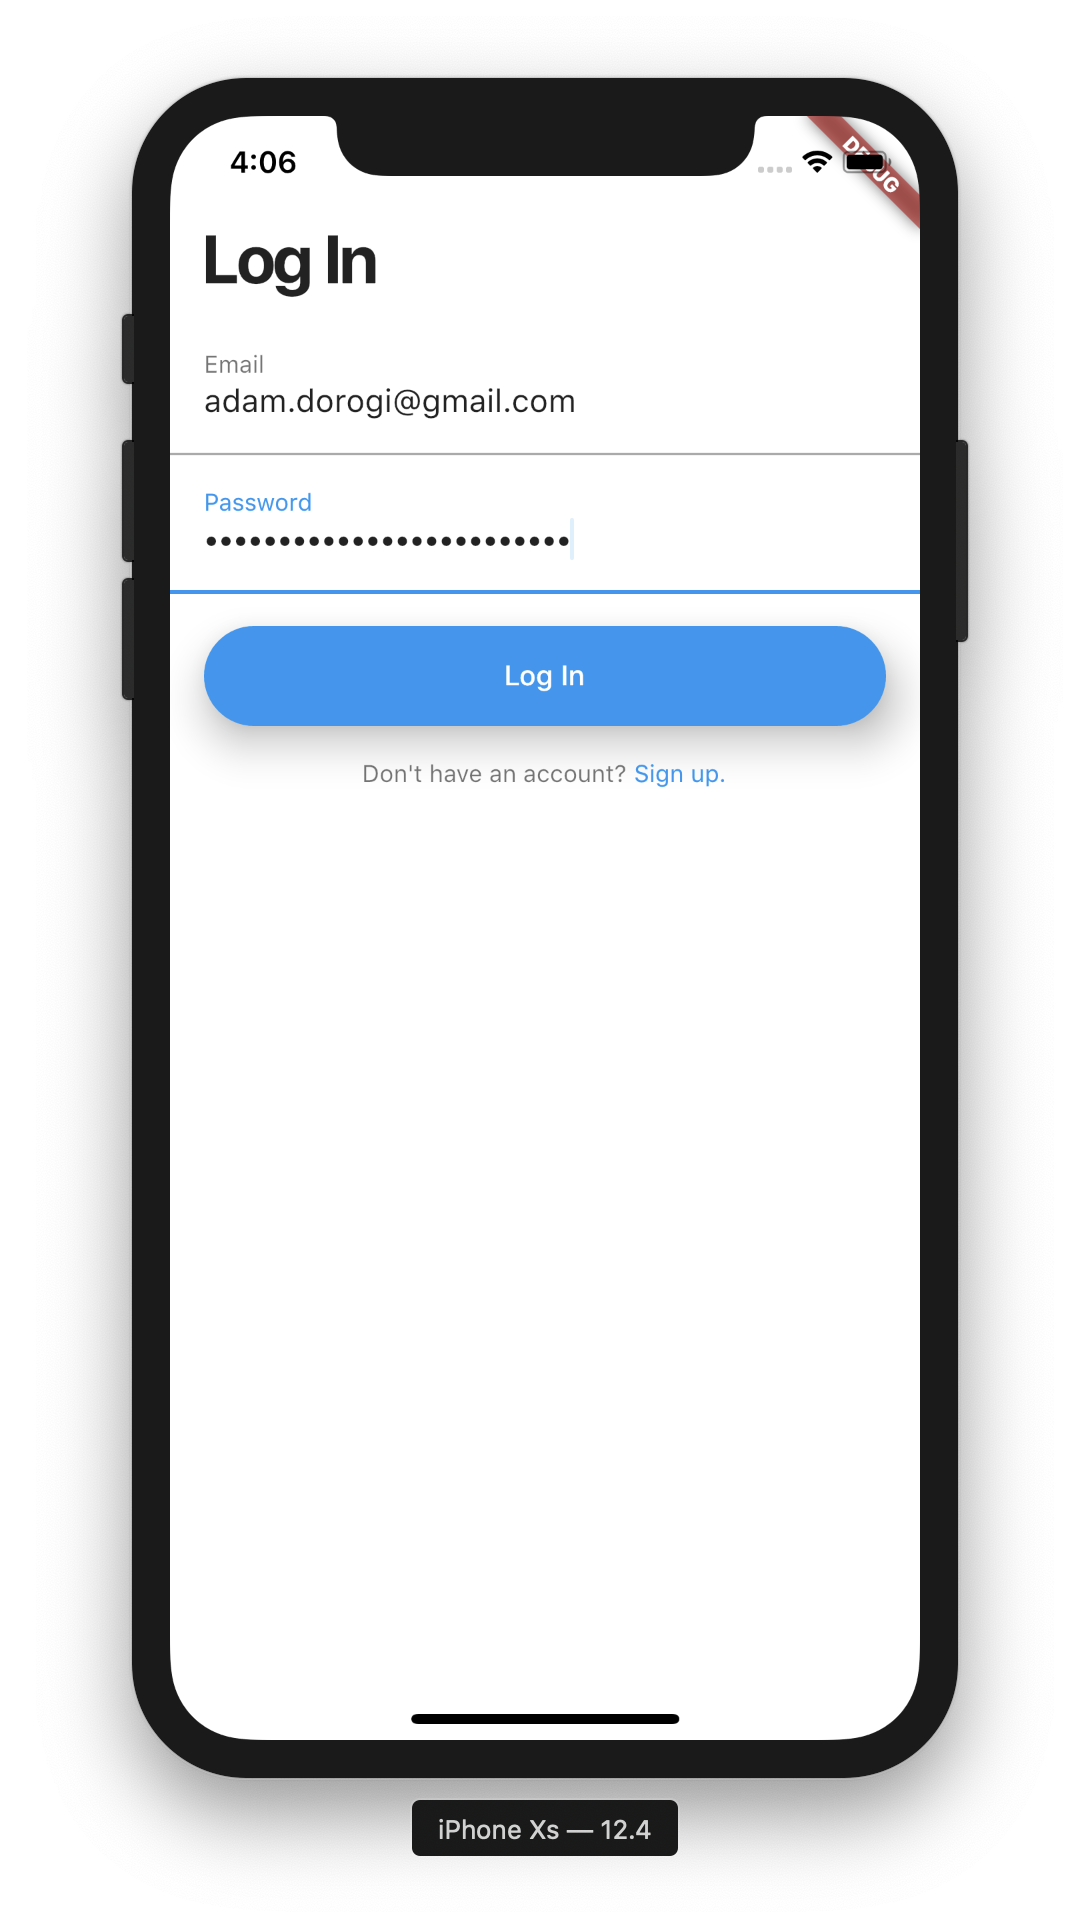
\includegraphics[width=\textwidth]{LogInScreen.png}
	\caption{Screenshot of log in screen}
	\label{fig:log_in_screen}
	\end{figure}

\begin{figure}[h]
\centering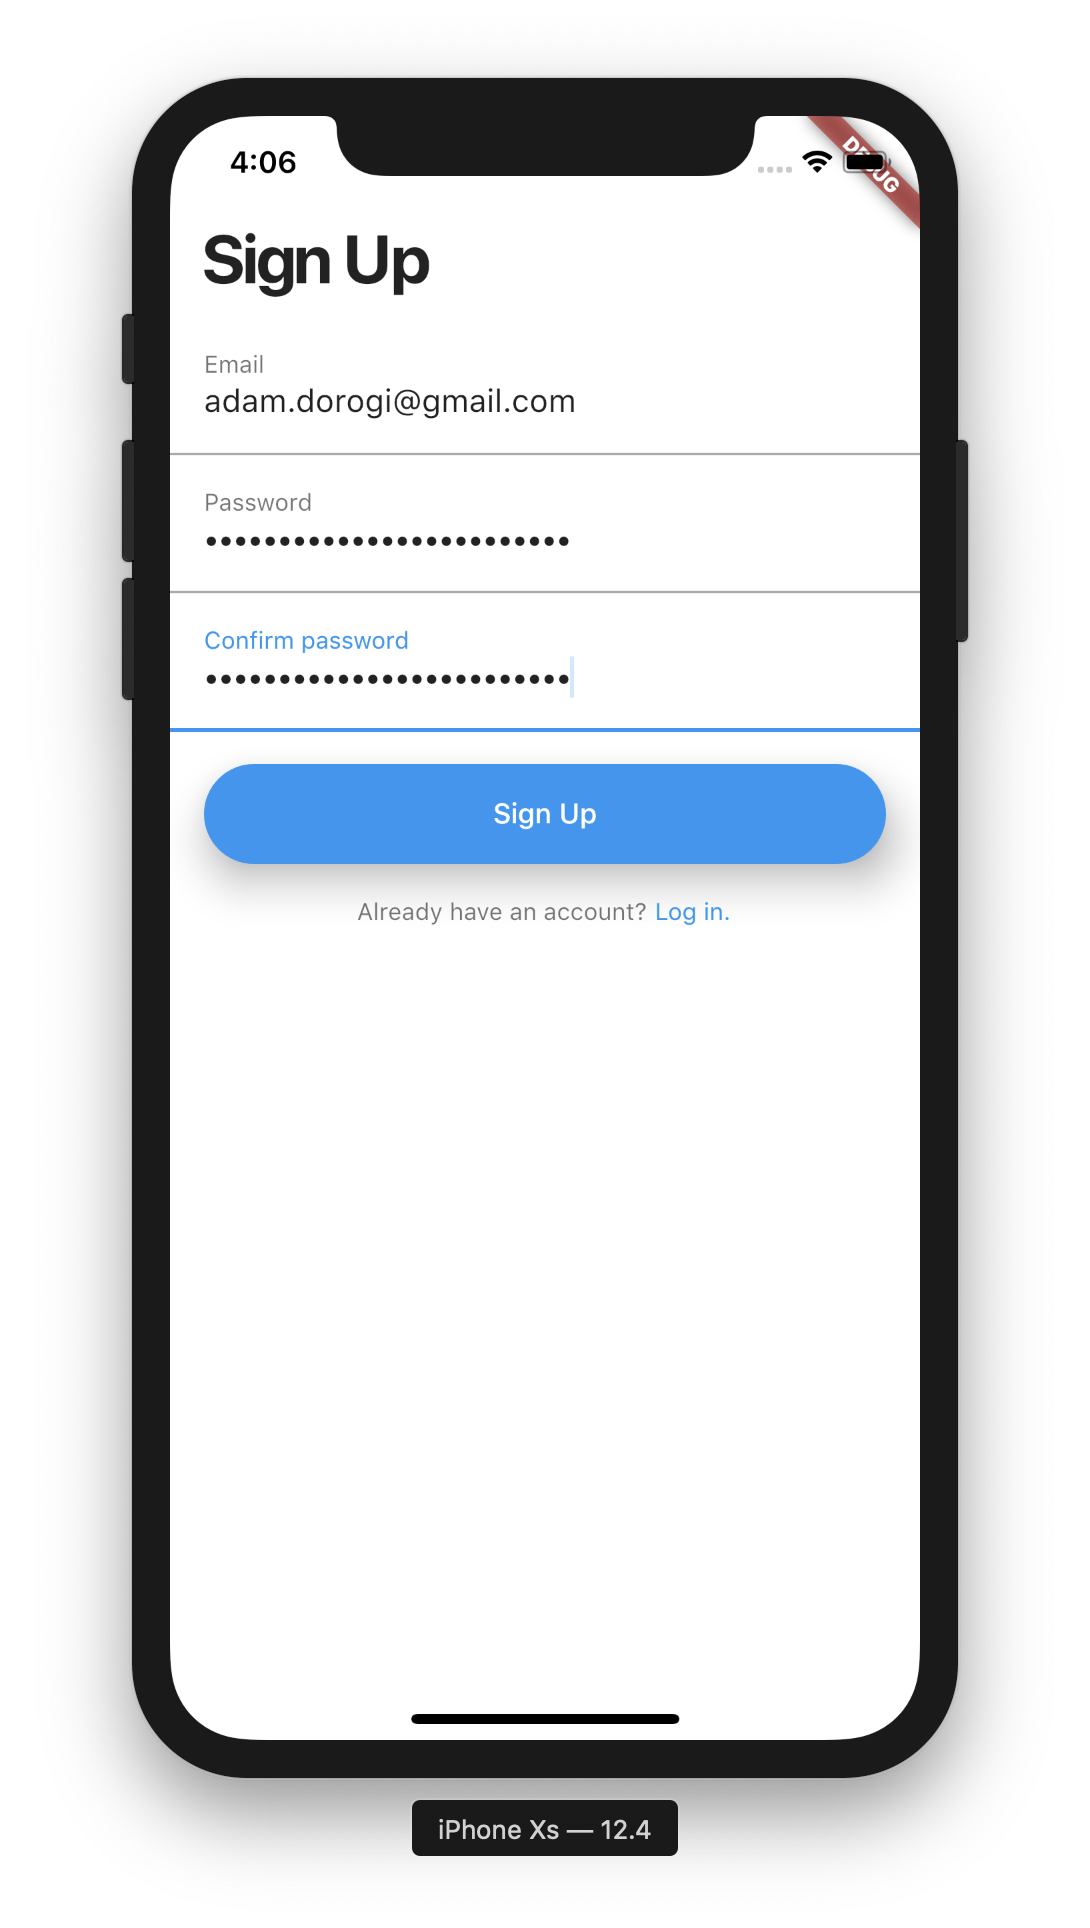
\includegraphics[width=\textwidth]{SignUpScreen.png}
\caption{Screenshot of sign up screen}
\label{fig:sign_up_screen}
\end{figure}

\begin{figure}[h]
	\centering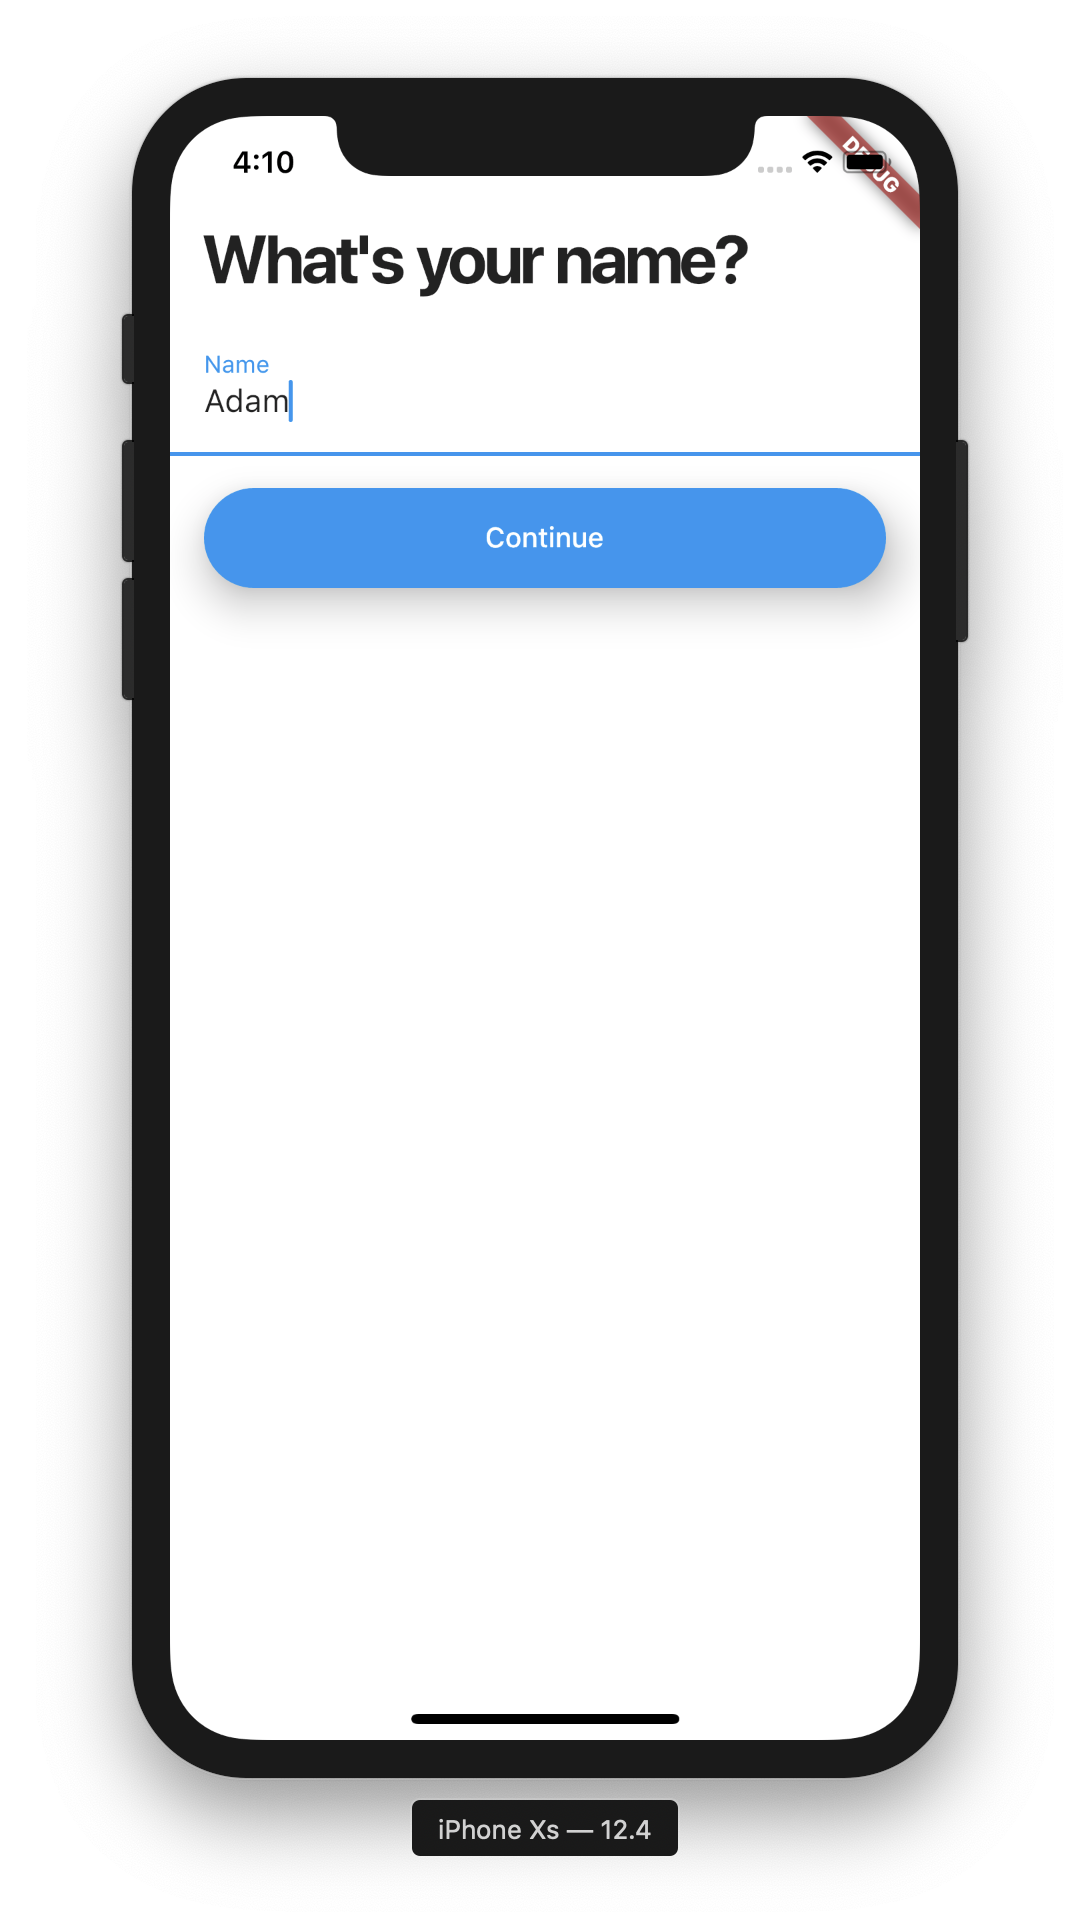
\includegraphics[width=\textwidth]{NameScreen.png}
	\caption{Screenshot of name screen at sign up}
	\label{fig:name_screen}
	\end{figure}

	\begin{figure}[h]
		\centering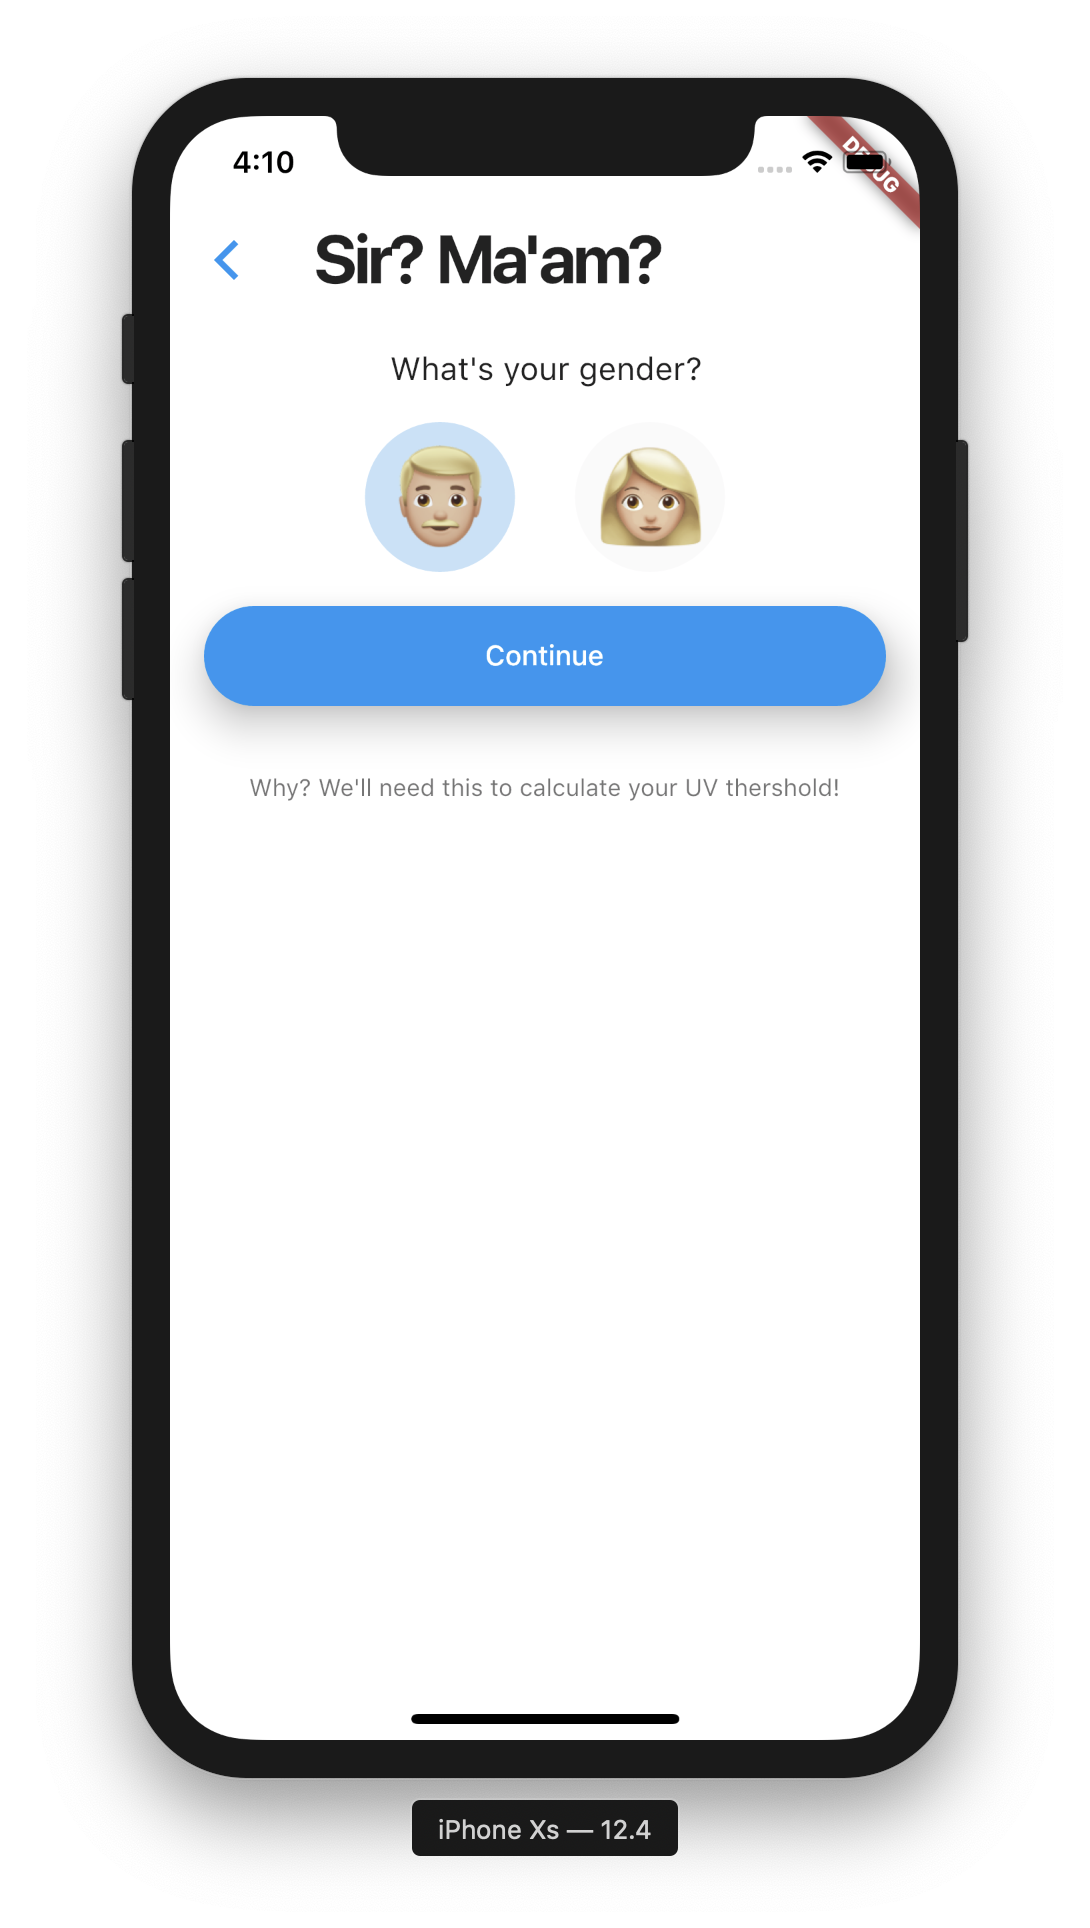
\includegraphics[width=\textwidth]{GenderScreen.png}
		\caption{Screenshot of gender screen at sign up}
		\label{fig:gender_screen}
		\end{figure}

\begin{figure}[h]
\centering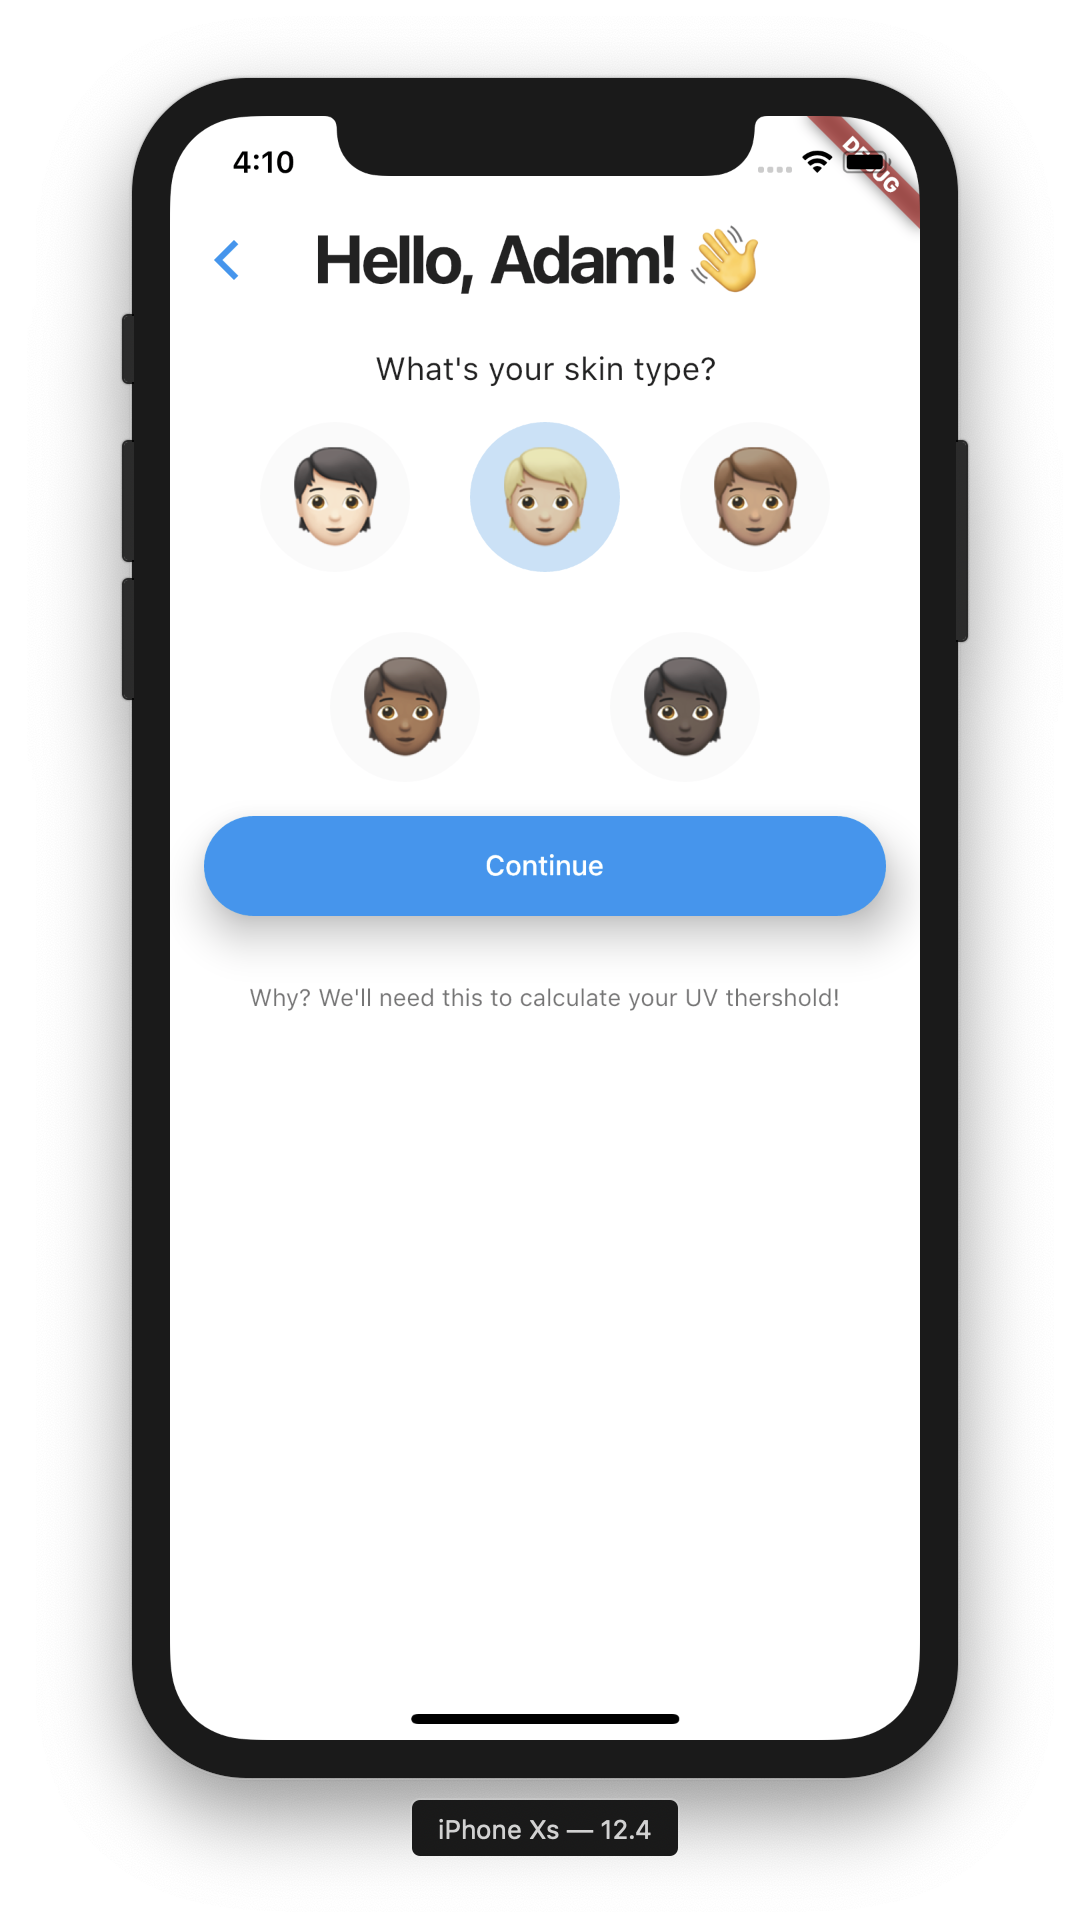
\includegraphics[width=\textwidth]{SkinTypeScreen.png}
\caption{Screenshot of skin type screen at sign up}
\label{fig:skin_type_screen}
\end{figure}

\begin{figure}[h]
	\centering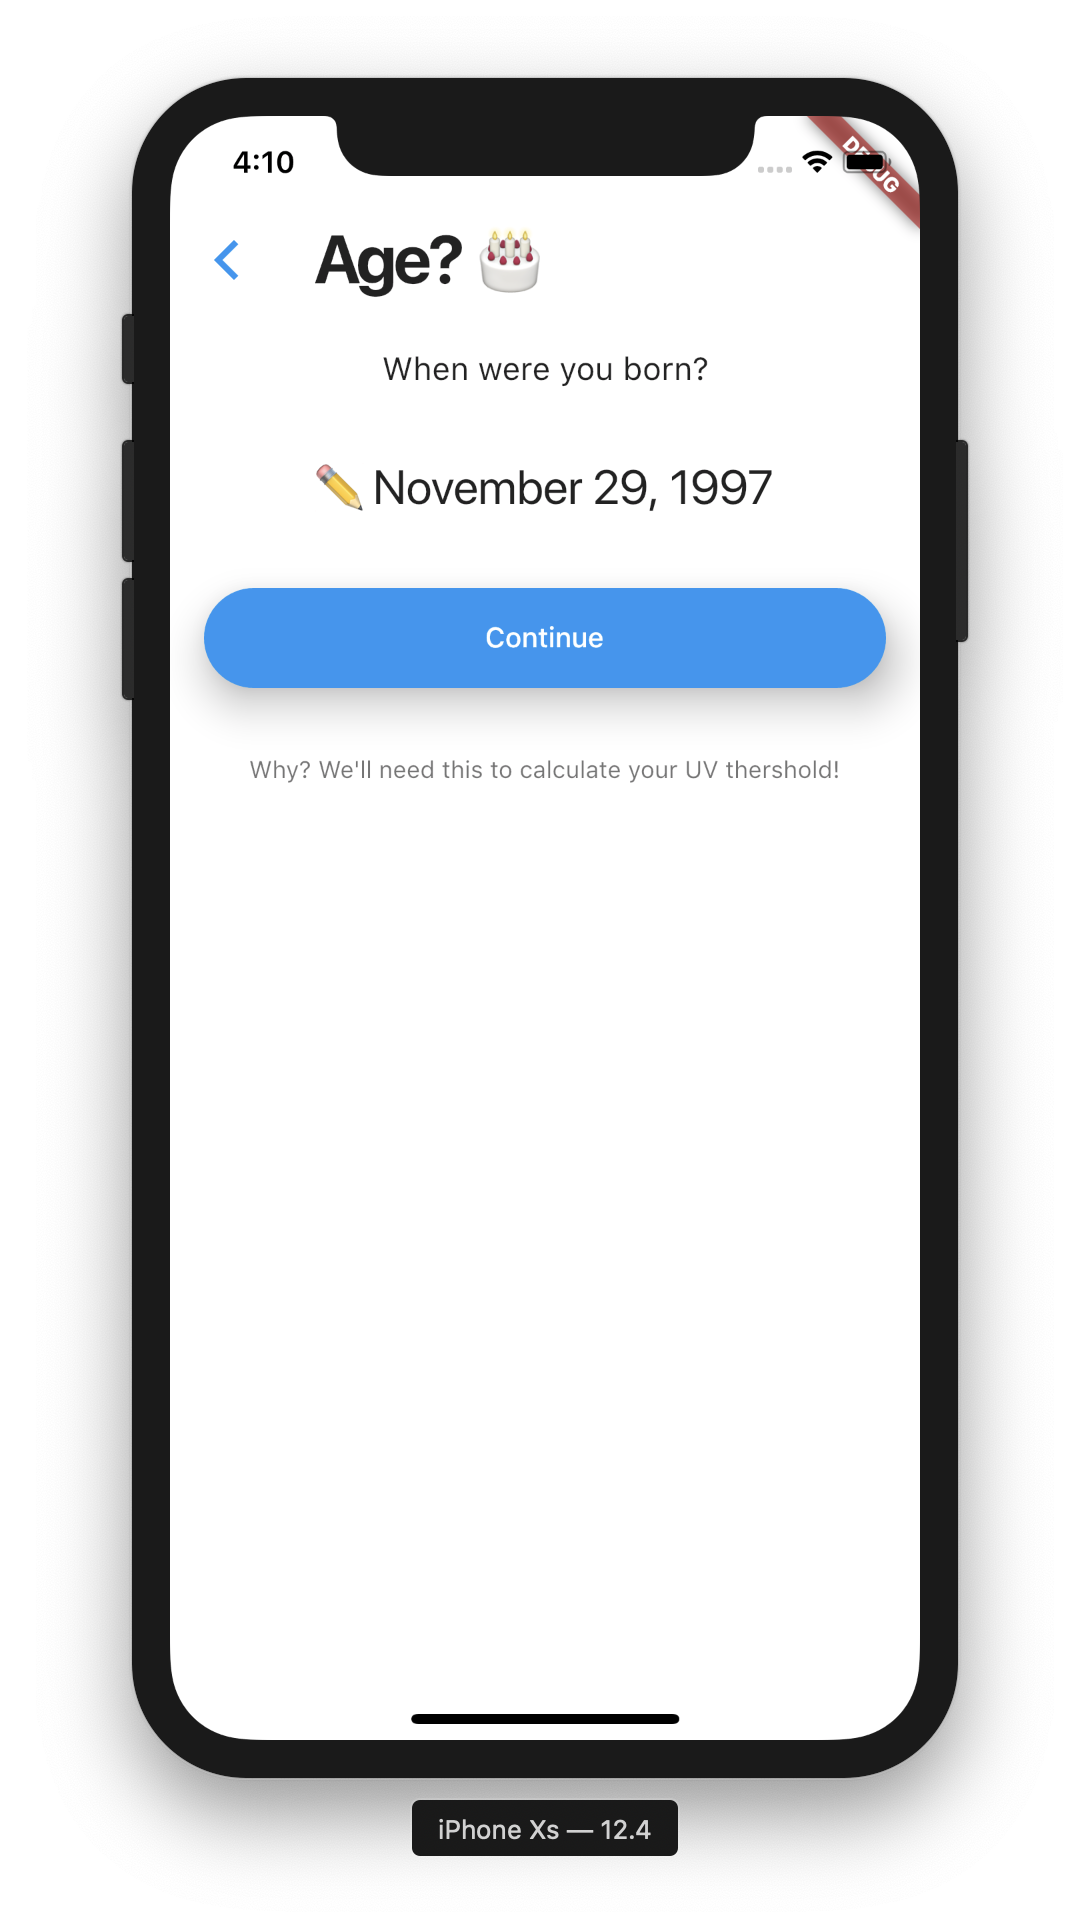
\includegraphics[width=\textwidth]{AgeScreen.png}
	\caption{Screenshot of age at sign up}
	\label{fig:age_screen}
	\end{figure}


\begin{figure}[h]
	\centering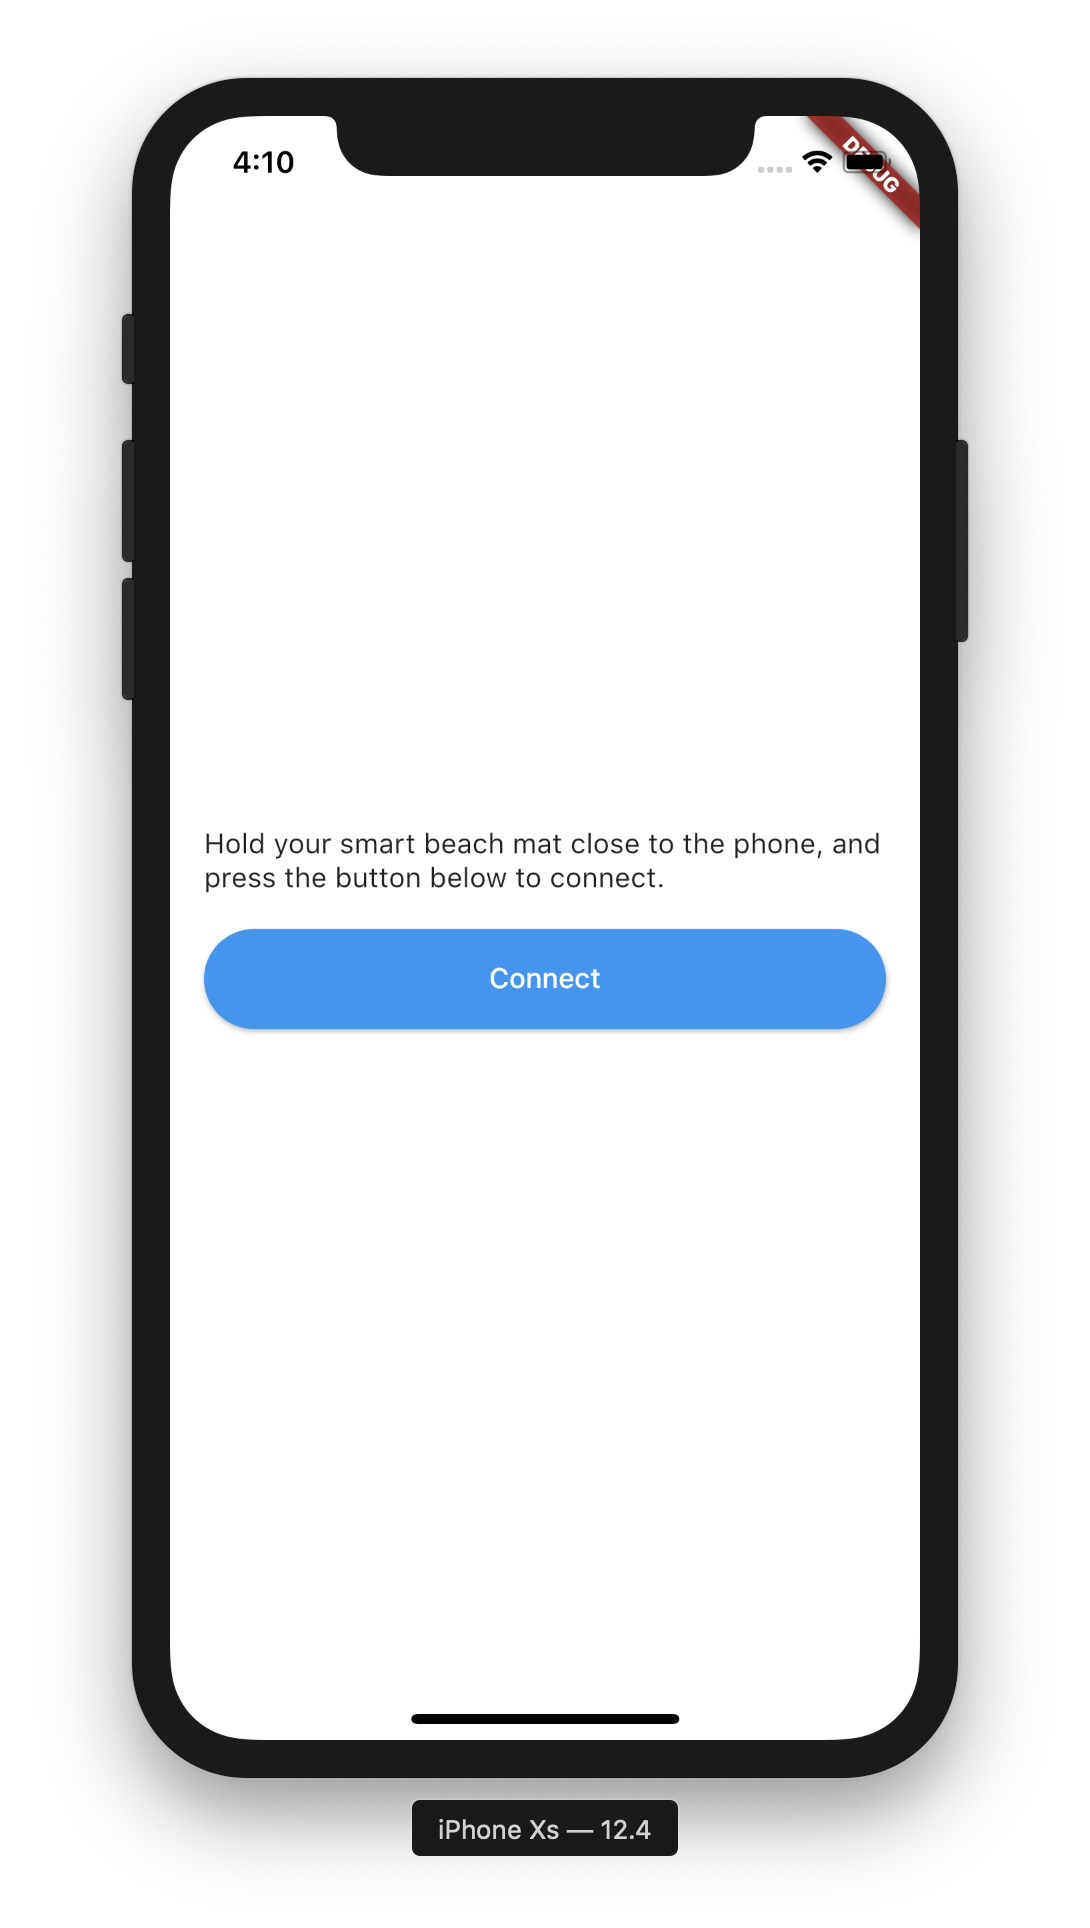
\includegraphics[width=\textwidth]{ConnectScreen.png}
	\caption{Screenshot of device connection screen}
	\label{fig:connect_screen}
	\end{figure}

	\begin{figure}[h]
		\centering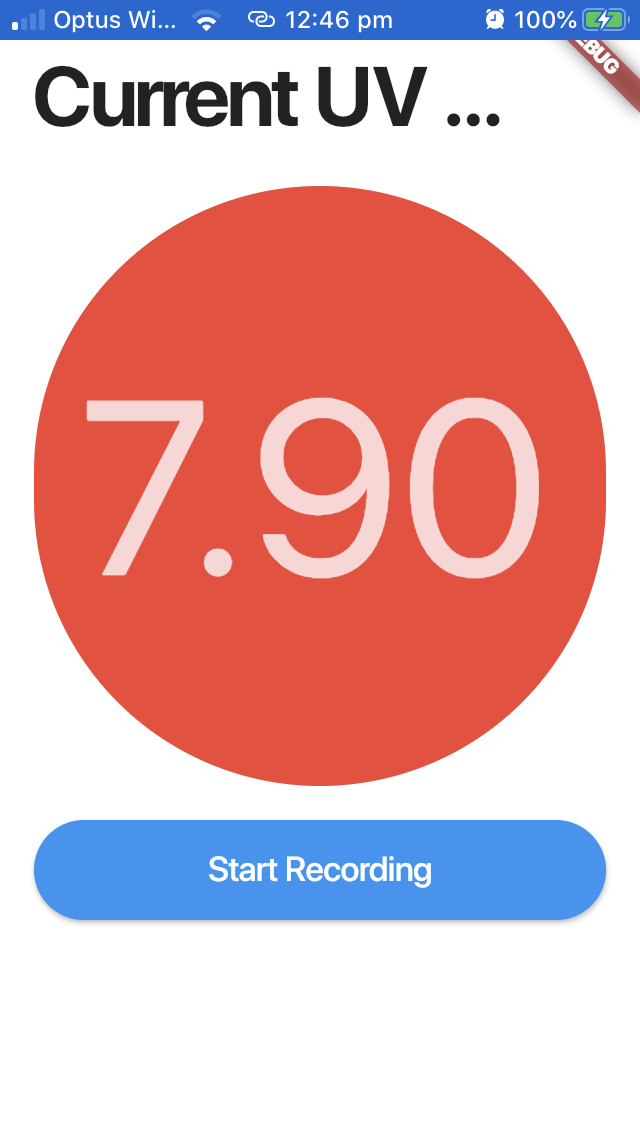
\includegraphics[width=\textwidth]{UVScreen.jpeg}
		\caption{Screenshot of UV screen}
		\label{fig:uv_screen}
		\end{figure}
		
	

\cleardoublepage

\chapter{Conclusions}

\textbf{Conclusion (15\%):} The results from the work should be analysed in a
fashion that highlights your comprehension and shows insight into the
significance of the results. The thesis should have a critical review of your
performance against the stated plan, including the stated goals and schedule.
The thesis should conclude with a clear concise summary of the outcomes of the
thesis (relating to your initial definitions and put in context of the
literature) and recommendations of how the work might be continued or improved.

\section{Summary and Conclusions}

\section{Future Work}
\label{secn:future_work}

\appendix

% Chapters after the \appendix command are lettered, not numbered.
% Setting apart the appendices in the table of contents is awkward:

\newpage
\addcontentsline{toc}{part}{Appendices}
\mbox{}
\newpage

% The \mbox{} command between two \newpage commands gives a blank page.
% In the contents, the ``Appendices'' heading is shown as being on this
% blank page, which is the page before the first appendix.  This stops the
% first appendix from be listed ABOVE the word ``Appendices'' in the
% table of contents.

% \include appendix chapters here.

\cleardoublepage

\chapter{Shade's iOS Application Screenshots}
\label{app:shade_screenshots}

\begin{figure}[h]
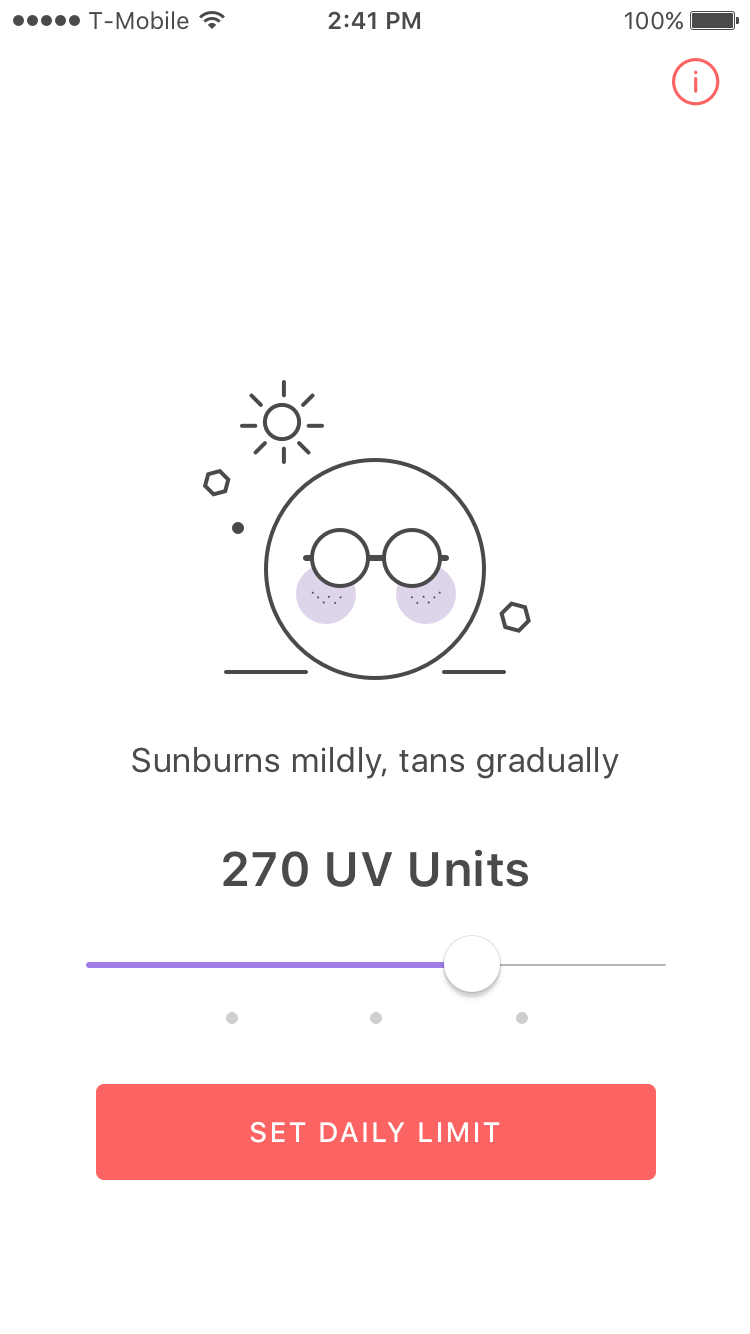
\includegraphics[width=\textwidth]{ShadeOnboarding.png}
\end{figure}

\begin{figure}[h]
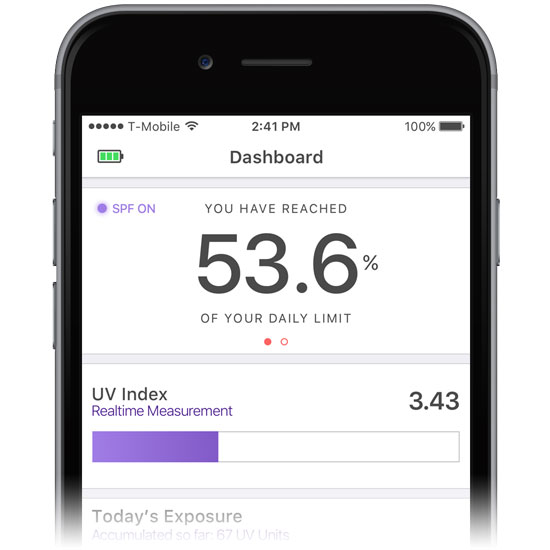
\includegraphics[width=\textwidth]{ShadeMeasurement.jpg}
\end{figure}

\chapter{QSun's iOS Application Screenshots}
\label{app:qsun_screenshots}

\begin{figure}[h]
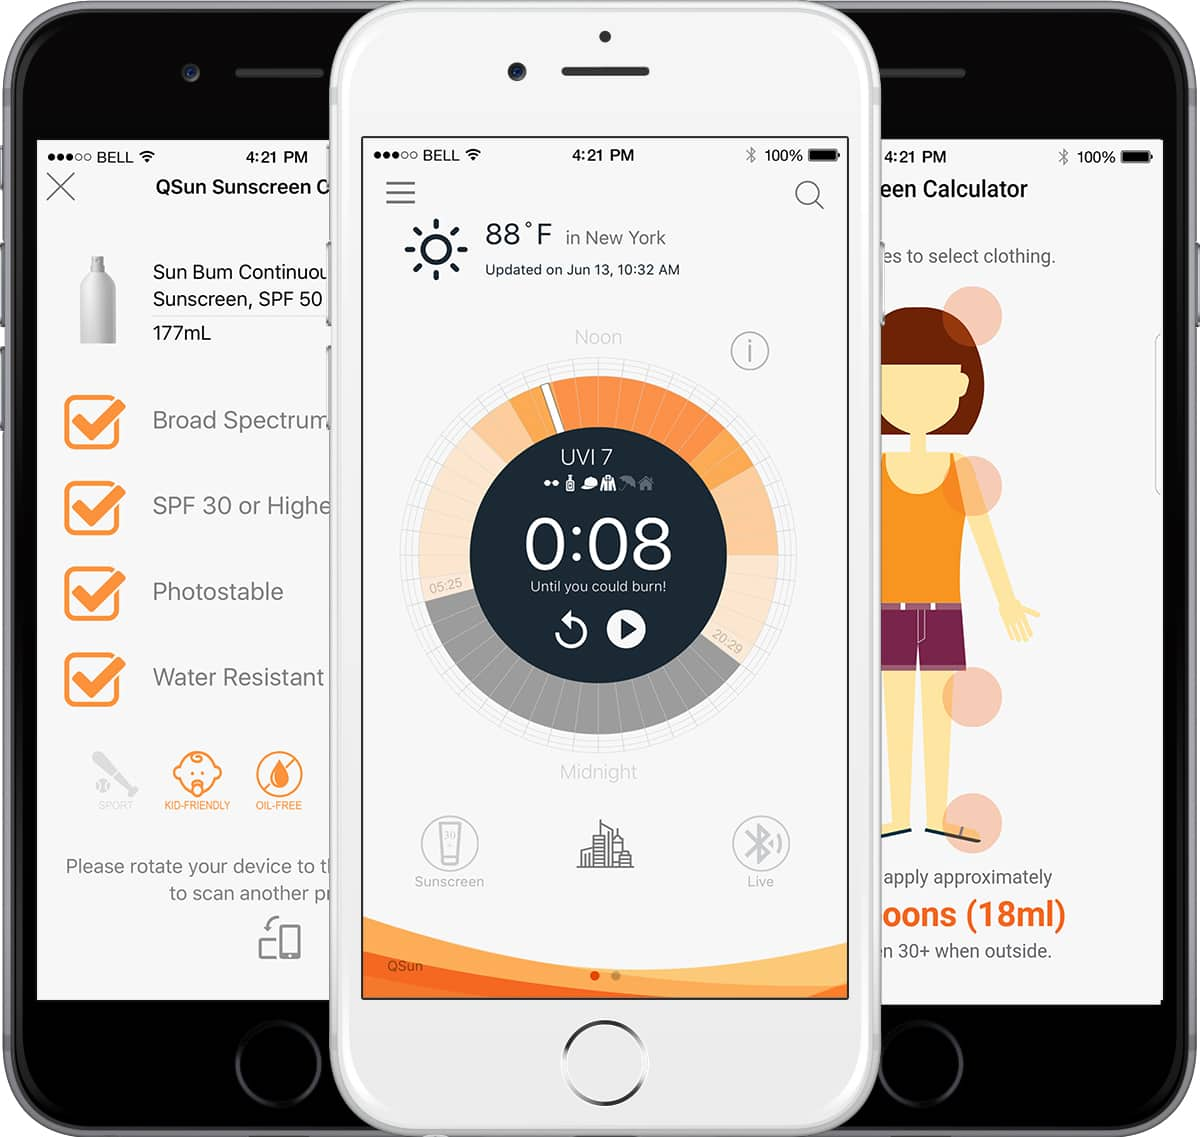
\includegraphics[width=\textwidth]{QSunApp.jpg}
\end{figure}

\chapter{Dummy appendix}

Appendices are useful for supplying necessary details or explanations
which do not seem to fit into the main text, perhaps because they are
too long and would distract the reader from the central argument.
Appendices are also used for program listings.

Notice that appendices are ``numbered'' with capital letters, not
numerals.  When the \verb+\appendix+ command in
\LaTeX~\cite[p.\,175]{lamport} is used with the \texttt{book} document
class, it causes subsequent chapters to be treated as appendices.

\chapter{Code Listings}

\section{\texttt{BLE\_write.ino}}
\label{code:ble_write}
\begin{lstlisting}[basicstyle=\ttfamily,breaklines=true,language=c++]
/*
Based on Neil Kolban example for IDF: https://github.com/nkolban/esp32-snippets/blob/master/cpp_utils/tests/BLE%20Tests/SampleWrite.cpp
Ported to Arduino ESP32 by Evandro Copercini
*/

#include <BLEDevice.h>
#include <BLEUtils.h>
#include <BLEServer.h>

// See the following for generating UUIDs:
// https://www.uuidgenerator.net/

#define SERVICE_UUID        "4fafc201-1fb5-459e-8fcc-c5c9c331914b"
#define CHARACTERISTIC_UUID "beb5483e-36e1-4688-b7f5-ea07361b26a8"


class MyCallbacks: public BLECharacteristicCallbacks {
    void onWrite(BLECharacteristic *pCharacteristic) {
      std::string value = pCharacteristic->getValue();

      if (value.length() > 0) {
        Serial.println("*********");
        Serial.print("New value: ");
        for (int i = 0; i < value.length(); i++)
          Serial.print(value[i]);

        Serial.println();
        Serial.println("*********");
      }
    }
};

void setup() {
  Serial.begin(115200);

  Serial.println("1- Download and install an BLE scanner app in your phone");
  Serial.println("2- Scan for BLE devices in the app");
  Serial.println("3- Connect to MyESP32");
  Serial.println("4- Go to CUSTOM CHARACTERISTIC in CUSTOM SERVICE and write something");
  Serial.println("5- See the magic =)");

  BLEDevice::init("MyESP32");
  BLEServer *pServer = BLEDevice::createServer();

  BLEService *pService = pServer->createService(SERVICE_UUID);

  BLECharacteristic *pCharacteristic = pService->createCharacteristic(
                                         CHARACTERISTIC_UUID,
                                         BLECharacteristic::PROPERTY_READ |
                                         BLECharacteristic::PROPERTY_WRITE
                                       );

  pCharacteristic->setCallbacks(new MyCallbacks());

  pCharacteristic->setValue("Hello World");
  pService->start();

  BLEAdvertising *pAdvertising = pServer->getAdvertising();
  pAdvertising->start();
}

void loop() {
  // put your main code here, to run repeatedly:
  delay(2000);
}
\end{lstlisting}

\section{\texttt{si1145test.ino}}
\label{code:si1145test}

\begin{lstlisting}[basicstyle=\ttfamily,breaklines=true,language=c++]
	/*************************************************** 
	This is a library for the Si1145 UV/IR/Visible Light Sensor
  
	Designed specifically to work with the Si1145 sensor in the
	adafruit shop
	----> https://www.adafruit.com/products/1777
  
	These sensors use I2C to communicate, 2 pins are required to  
	interface
	Adafruit invests time and resources providing this open source code, 
	please support Adafruit and open-source hardware by purchasing 
	products from Adafruit!
  
	Written by Limor Fried/Ladyada for Adafruit Industries.  
	BSD license, all text above must be included in any redistribution
   ****************************************************/
  
  #include <Wire.h>
  #include "Adafruit_SI1145.h"
  
  Adafruit_SI1145 uv = Adafruit_SI1145();
  
  void setup() {
	Serial.begin(9600);
	
	Serial.println("Adafruit SI1145 test");
	
	if (! uv.begin()) {
	  Serial.println("Didn't find Si1145");
	  while (1);
	}
  
	Serial.println("OK!");
  }
  
  void loop() {
	Serial.println("===================");
	Serial.print("Vis: "); Serial.println(uv.readVisible());
	Serial.print("IR: "); Serial.println(uv.readIR());
	
	// Uncomment if you have an IR LED attached to LED pin!
	//Serial.print("Prox: "); Serial.println(uv.readProx());
  
	float UVindex = uv.readUV();
	// the index is multiplied by 100 so to get the
	// integer index, divide by 100!
	UVindex /= 100.0;  
	Serial.print("UV: ");  Serial.println(UVindex);
  
	delay(1000);
  }
\end{lstlisting}

\section{\texttt{smart\_beachmat\_hardware.ino}}
\label{code:final}
\begin{lstlisting}[basicstyle=\ttfamily,breaklines=true,language=c++]
/*************************************************** 
  This is a library for the Si1145 UV/IR/Visible Light Sensor

  Designed specifically to work with the Si1145 sensor in the
  adafruit shop
  ----> https://www.adafruit.com/products/1777

  These sensors use I2C to communicate, 2 pins are required to  
  interface
  Adafruit invests time and resources providing this open source code, 
  please support Adafruit and open-source hardware by purchasing 
  products from Adafruit!

  Written by Limor Fried/Ladyada for Adafruit Industries.  
  BSD license, all text above must be included in any redistribution
 ****************************************************/
/*
    Video: https://www.youtube.com/watch?v=oCMOYS71NIU
    Based on Neil Kolban example for IDF: https://github.com/nkolban/esp32-snippets/blob/master/cpp_utils/tests/BLE%20Tests/SampleNotify.cpp
    Ported to Arduino ESP32 by Evandro Copercini
    updated by chegewara

   Create a BLE server that, once we receive a connection, will send periodic notifications.
   The service advertises itself as: 4fafc201-1fb5-459e-8fcc-c5c9c331914b
   And has a characteristic of: beb5483e-36e1-4688-b7f5-ea07361b26a8

   The design of creating the BLE server is:
   1. Create a BLE Server
   2. Create a BLE Service
   3. Create a BLE Characteristic on the Service
   4. Start the service.
   5. Start advertising.

   A connect hander associated with the server starts a background task that performs notification
   every couple of seconds.
*/

/* TODO:
 * - remove `print...` functions.
 */

// Bluetooth
#include <BLEDevice.h>
#include <BLEServer.h>
#include <BLEUtils.h>
#include <BLE2902.h>

// UV sensing
#include <Wire.h>
#include "Adafruit_SI1145.h"

// BLE service UUIDs (https://www.bluetooth.com/specifications/gatt/services)
#define ENVIRONMENTAL_SENSING_SERVICE_UUID "181A"
#define BATTERY_SERVICE_UUID               "180F"

// BLE characteristic UUIDs (https://www.bluetooth.com/specifications/gatt/characteristics)
#define UV_INDEX_CHARACTERISTIC_UUID      "2A76"
#define BATTERY_LEVEL_CHARACTERISTIC_UUID "2A19"

// Time periods
#define NOTIFICATION_PERIOD 5000


BLEServer* pServer;
BLECharacteristic* uvIndexCharacteristic;
BLECharacteristic* batteryLevelCharacteristic;
BLEAdvertising* deviceAdvertising;

Adafruit_SI1145 sensor;

bool isConnected = false;

/*
 * Callbacks associated with the operation of a `BLEServer`.
 */
class ServerCallbacks: public BLEServerCallbacks {
  /*
   * Handle a new client connection.
   */
  void onConnect(BLEServer* pServer) {
    isConnected = true;
    Serial.println("Device connected.");
  }

  /*
   * Handle an existing client disconnection.
   */
  void onDisconnect(BLEServer* pServer) {
    isConnected = false;
    Serial.println("Device disconnected.");
  }
};

/*
 * Run once, after each powerup or reset of the device.
 */
void setup() {
  Serial.begin(115200);
  
  // Check for UV sensor.
  sensor = Adafruit_SI1145();
  while (!sensor.begin());
  Serial.println("UV sensor detected.");

  // Create the BLE device.
  BLEDevice::init("Smart Beach Mat");

  // Create the BLE server.
  pServer = BLEDevice::createServer();
  pServer->setCallbacks(new ServerCallbacks());

  // Create the BLE environmental sensing service.
  BLEService* environmentalSensingService = pServer->createService(ENVIRONMENTAL_SENSING_SERVICE_UUID);

  // Create the BLE UV index characteristic.
  uvIndexCharacteristic = environmentalSensingService->createCharacteristic(
                            UV_INDEX_CHARACTERISTIC_UUID,
                            BLECharacteristic::PROPERTY_NOTIFY
                          );

  // Start the environmental sensing service.
  environmentalSensingService->start();

  // Create the BLE battery service.
  BLEService* batteryService = pServer->createService(BATTERY_SERVICE_UUID);

  // Create the BLE battery level characteristic.
  batteryLevelCharacteristic = batteryService->createCharacteristic(
                            BATTERY_LEVEL_CHARACTERISTIC_UUID,
                            BLECharacteristic::PROPERTY_NOTIFY
                          );

  // Start the battery service.
  batteryService->start();

  // Set up advertisement.
  deviceAdvertising = BLEDevice::getAdvertising();
  deviceAdvertising->setScanResponse(false);
  deviceAdvertising->addServiceUUID(ENVIRONMENTAL_SENSING_SERVICE_UUID);
  deviceAdvertising->addServiceUUID(BATTERY_SERVICE_UUID);
  deviceAdvertising->start();
}

/*
 * Loop continuously while the device is powered on.
 */
void loop() {
  // Notify connected device of UV index.
  if (isConnected) {
    float uvIndex = sensor.readUV() / 100.0;
    int batteryLevel = 40;

    Serial.print("UV: ");  Serial.println(uvIndex);
    Serial.print("BATTERY: ");  Serial.println(batteryLevel);
    
    uvIndexCharacteristic->setValue(uvIndex);
    uvIndexCharacteristic->notify();

    batteryLevelCharacteristic->setValue(batteryLevel);
    batteryLevelCharacteristic->notify();
    
    delay(NOTIFICATION_PERIOD);
  }
}
\end{lstlisting}

\section{Etc.}

\chapter{Companion disk}

If you wish to make some computer files available to your examiners,
you can list and describe the files here.  The files can be supplied
on a disk and inserted in a pocket fixed to the inside back cover.

The disk will not be needed if you can specify a URL from which the
files can be downloaded.

\cleardoublepage

% \begin{thebibliography}{99}
\addcontentsline{toc}{chapter}{Bibliography}

\bibliographystyle{unsrt}
\bibliography{thebibliography}
% \end{thebibliography}

\end{document}
